\documentclass[pdf]{beamer}
\mode<presentation>{}
\usepackage{minted}
\usepackage{tikz}
\usepackage{pgffor} %% gives looping with \foreach
\usepackage[absolute,overlay]{textpos}
\usepackage{lmodern} %% scalable latin characters
\usetikzlibrary{arrows,shapes,backgrounds}
\usepackage{multirow}
\usepackage{listings} %% another package for code related stuff


%% stuff for minted
\definecolor{mintedBg}{rgb}{0.95, 0.95, 0.95}
\definecolor{blockBg}{rgb}{0.6, 0.6, 0.95}
\definecolor{rnaColor}{rgb}{0, 0.6, 0}
\definecolor{cdsColor}{rgb}{0, 0.4, 0.4}
\definecolor{rnaPol}{rgb}{0.8,0,0.8}
\definecolor{ribosomeCol}{rgb}{0.5,0.5,0.1}
\definecolor{protColor}{rgb}{0.6,0,0.6}
%% colours for nucleotides:
\definecolor{dACol}{rgb}{0.5, 0.5, 0}
\definecolor{dCCol}{rgb}{0.8, 0, 0}
\definecolor{dGCol}{rgb}{0, 0.8, 0}
\definecolor{dTCol}{rgb}{0, 0, 0.8}

\definecolor{navy}{rgb}{0, 0, 0.6}
\definecolor{pur}{rgb}{0, 0, 0.6}
\definecolor{pyr}{rgb}{0.6, 0, 0.2}
%% define styles for different codes
\newminted{cpp}{linenos, bgcolor=mintedBg, fontsize=\footnotesize}
%% then use \begin{cppcode}
\newminted{c}{linenos, bgcolor=mintedBg, fontsize=\footnotesize}
\newminted{perl}{linenos, bgcolor=mintedBg, fontsize=\tiny}
\newminted{sh}{linenos, bgcolor=mintedBg, fontsize=\footnotesize,
  language=bash}
\newminted{console}{linenos, bgcolor=mintedBg, fontsize=\tiny}

%% a command to define a subheading
\newcommand\subHeading[1]{
  \par\bigskip {\Large\bfseries#1}\par\smallskip
}

%% I detest indentation in footnotes etc, so try this:
\makeatletter
\renewcommand\@makefntext[1]{\noindent\makebox[0em][r]{\@makefnmark}\tiny#1}
\makeatother
%% the makeatletter and makeatother are required to allow me to
%% to change the macro beginning with an @. (though when I call it
%% I don't use the @ ... 

\setlength\parskip{0.5em}
\setlength\parindent{0ex}

%% to have footnotes without references. This from tex.stackexchange.com
\newcommand\blfootnote[1]{%
  \begingroup  %% this makes it a local redefinition
  \renewcommand\thefootnote{}\footnote{#1}%
  \addtocounter{footnote}{-1}  % this adjusts the footnote counter
  \endgroup
}


\title{Tools for sequence analysis}
\subtitle{online \& offline}
\author{Martin Jakt}

\begin{document}

\begin{frame}
  \titlepage
\end{frame}

\begin{frame}{Online tools}
  Web frontends to sequence analysis programs:

  \begin{itemize}
  \item Easy to enter and run small number of analyses
  \item Provide web-formated graphical results (usually images)
  \item May allow download of vector based graphics / raw results
  \item Not convenient for more than a few simple analyses
  \item Using the results often involve reformatting editing on a local
    computer
  \item Both input and output may have to be reformatted for specific purposes
    / services: still useful to write your own programs
  \end{itemize}
\end{frame}

\begin{frame}[fragile]{tasks}
  \begin{itemize}
  \item global or local sequence alignment
    \begin{itemize}
    \item Smith-Waterman, Needleman-Wunsch, terminal gap penalties, etc...
    \item substitution matrix choice, gap insertion, gap penalties
    \end{itemize}
  \item visualisation (eg. dotplot, etc) or alignment
  \item Nucleotide / protein
  \item Database searches
  \item Multiple sequence alignment
  \item Phylogeny
  \item blast / blat
    \begin{itemize}
    \item blast subtypes, eg. PSI blast, 
    \item database choice
    \end{itemize}
  \end{itemize}
\end{frame}

\begin{frame}{Places to find tools}
  \begin{itemize}
  \item NCBI \url{https://www.ncbi.nlm.nih.gov/guide/sequence-analysis/}
  \item EBI \url{http://www.ebi.ac.uk/services}
  \item ExPASy \url{http://www.expasy.org/genomics/sequence_alignment}
    (external links)
  \item TCOFFEE \url{http://tcoffee.crg.cat/apps/tcoffee/index.html}
    (primarily multiple alignment)
  \end{itemize}
\end{frame}

\begin{frame}{You may like}
  \url{https://www.ncbi.nlm.nih.gov/tools/gbench/}
  \begin{figure}[ht]
    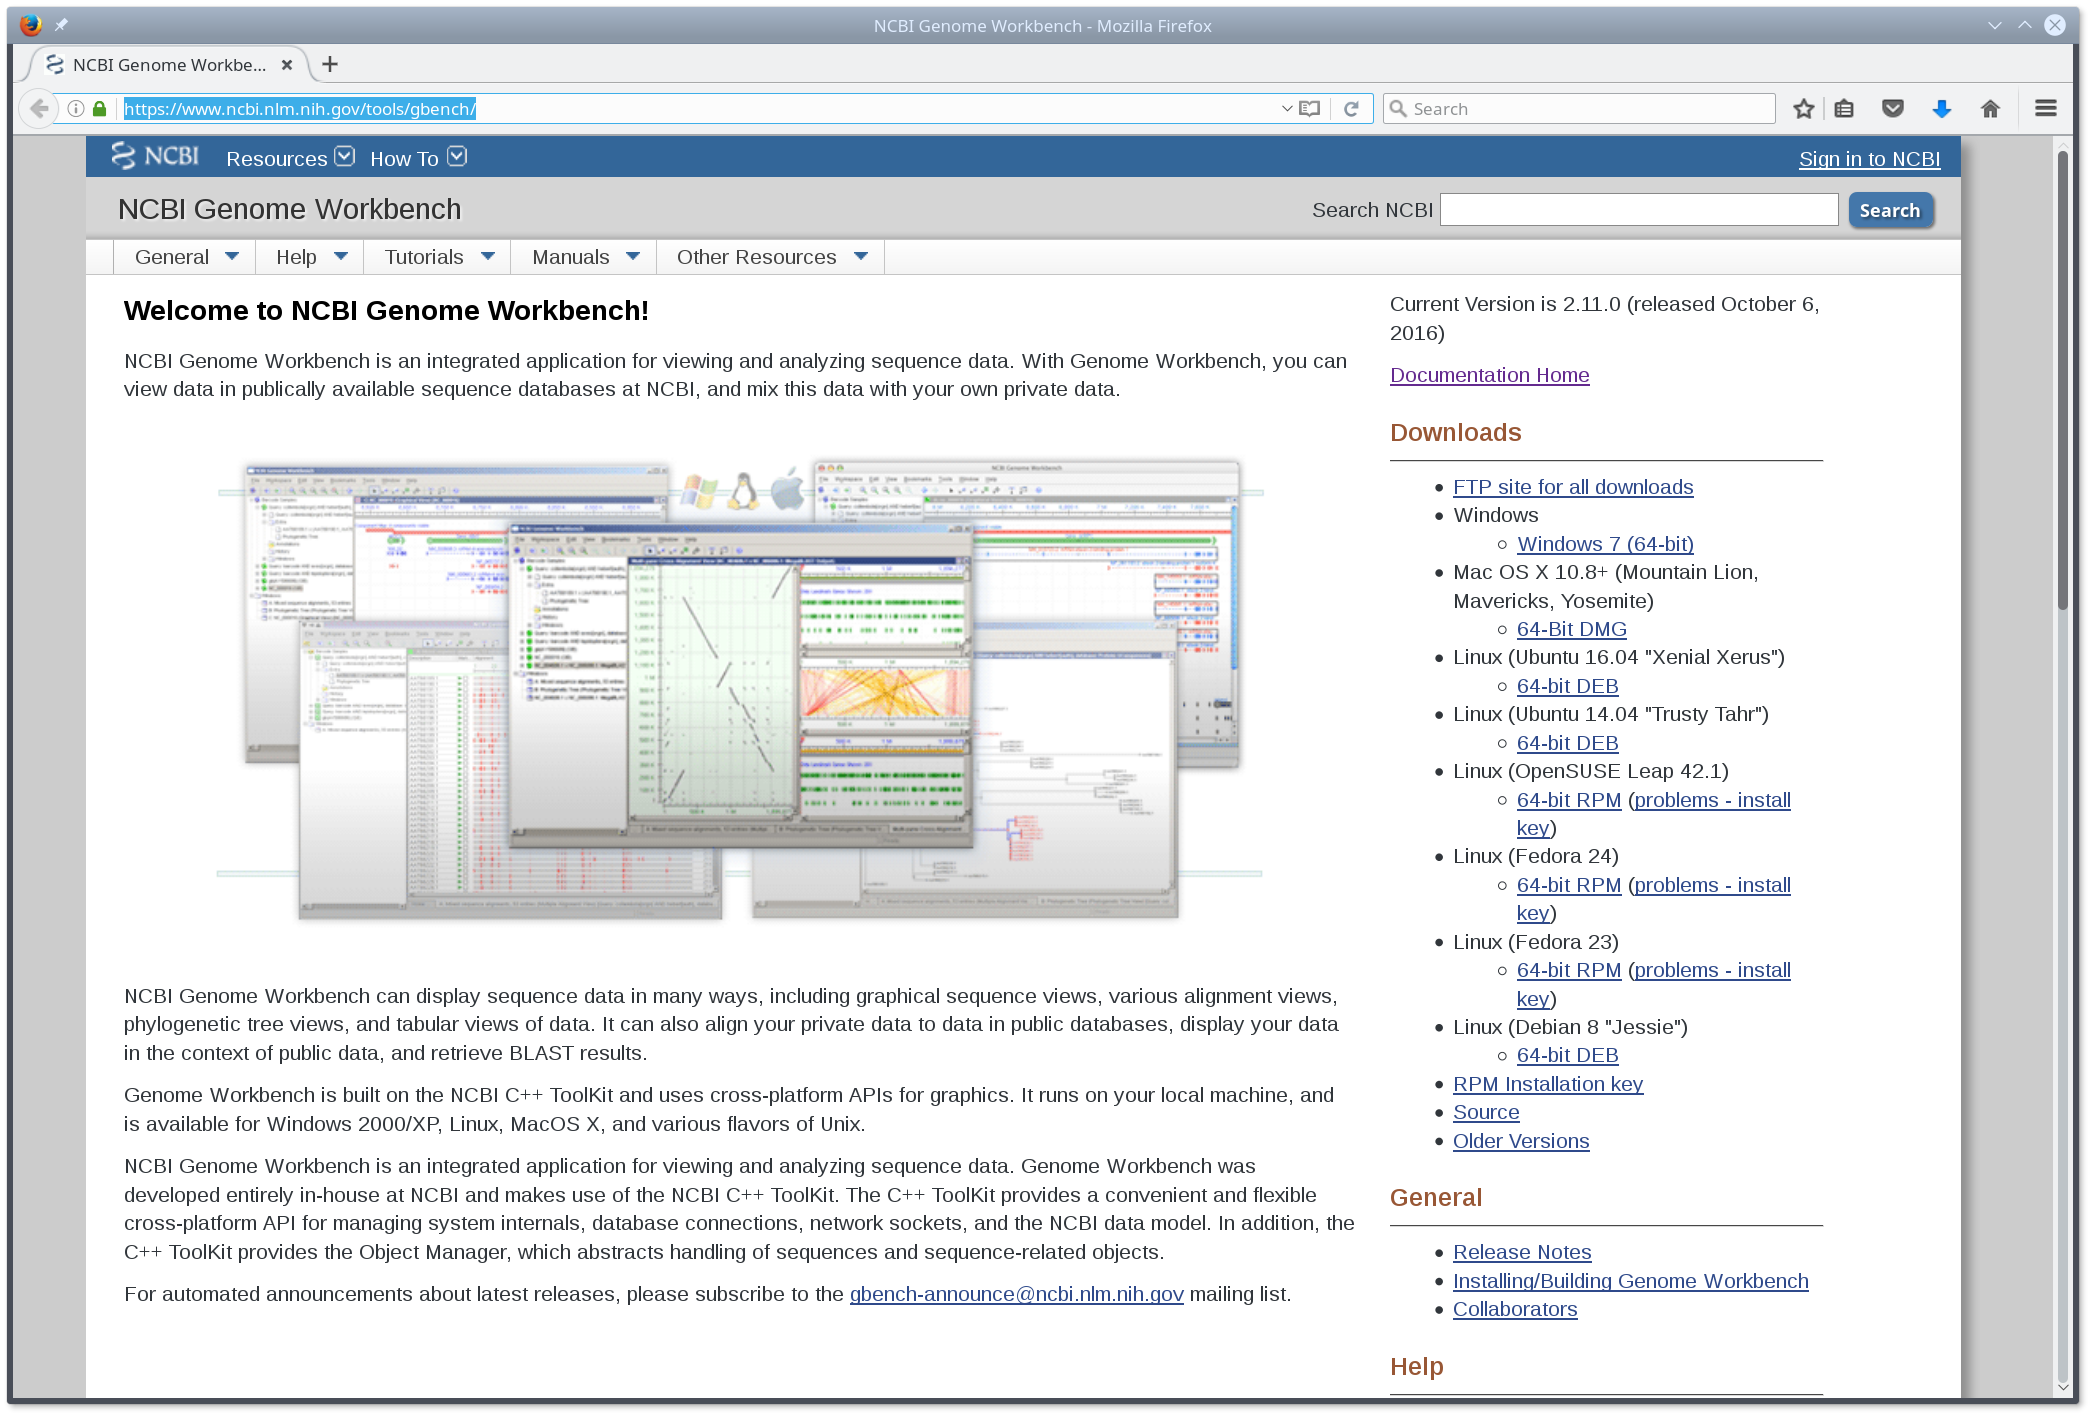
\includegraphics[width=0.7\textwidth]{images/NCBI_genome_work_bench}
  \end{figure}
\end{frame}

\begin{frame}{I like:}
  \url{ftp://ftp.ncbi.nlm.nih.gov/blast/executables/blast+/}
  \begin{figure}[ht]
    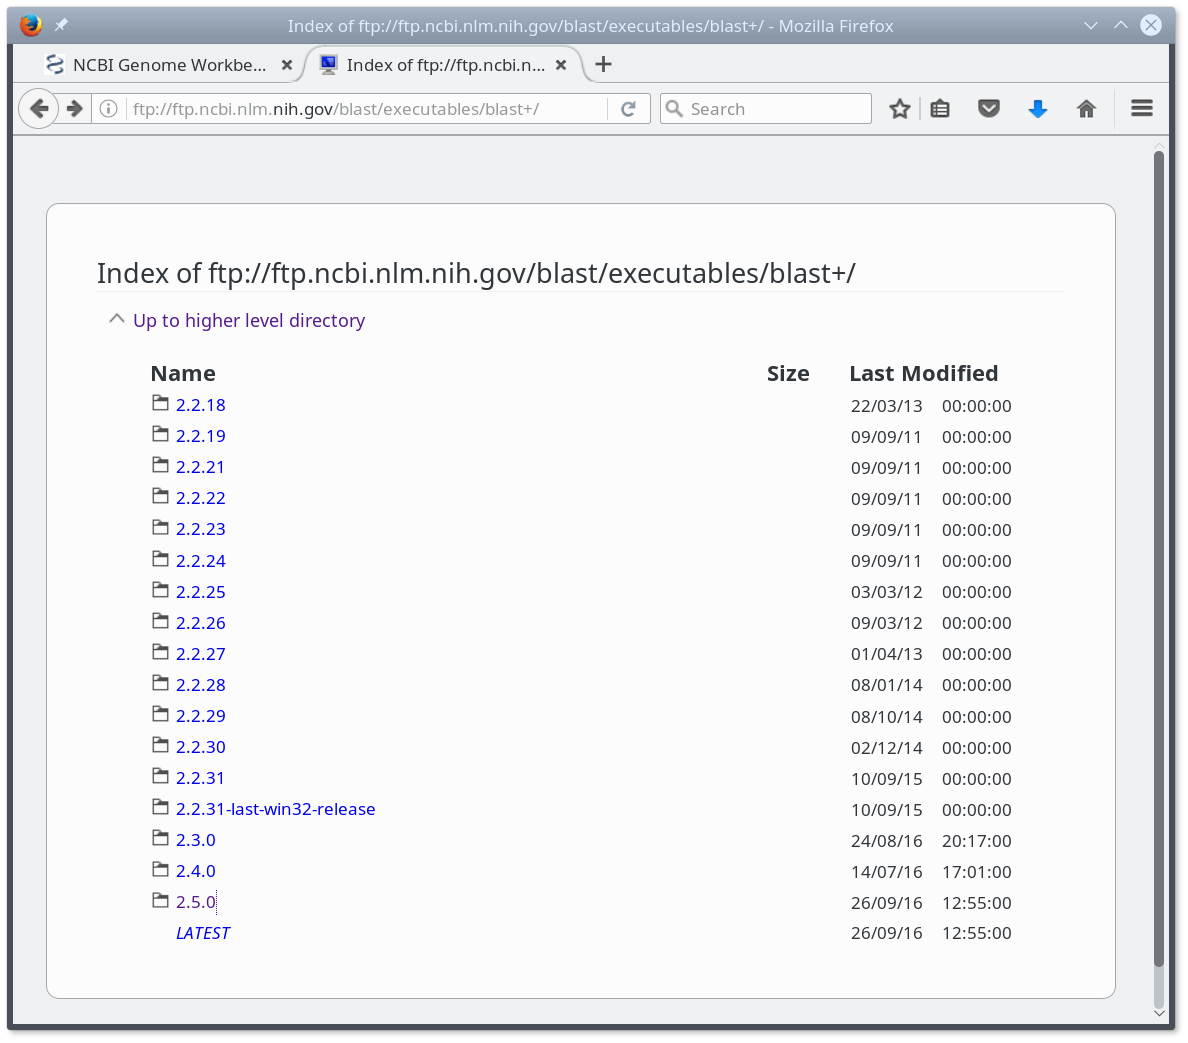
\includegraphics[width=0.7\textwidth]{images/ncbi_blast_download_page.png}
  \end{figure}
  even available for Windows
\end{frame}

\begin{frame}{NCBI tools}
  A big selection at:
  \url{https://www.ncbi.nlm.nih.gov/guide/sequence-analysis/}
  \begin{figure}[ht]
    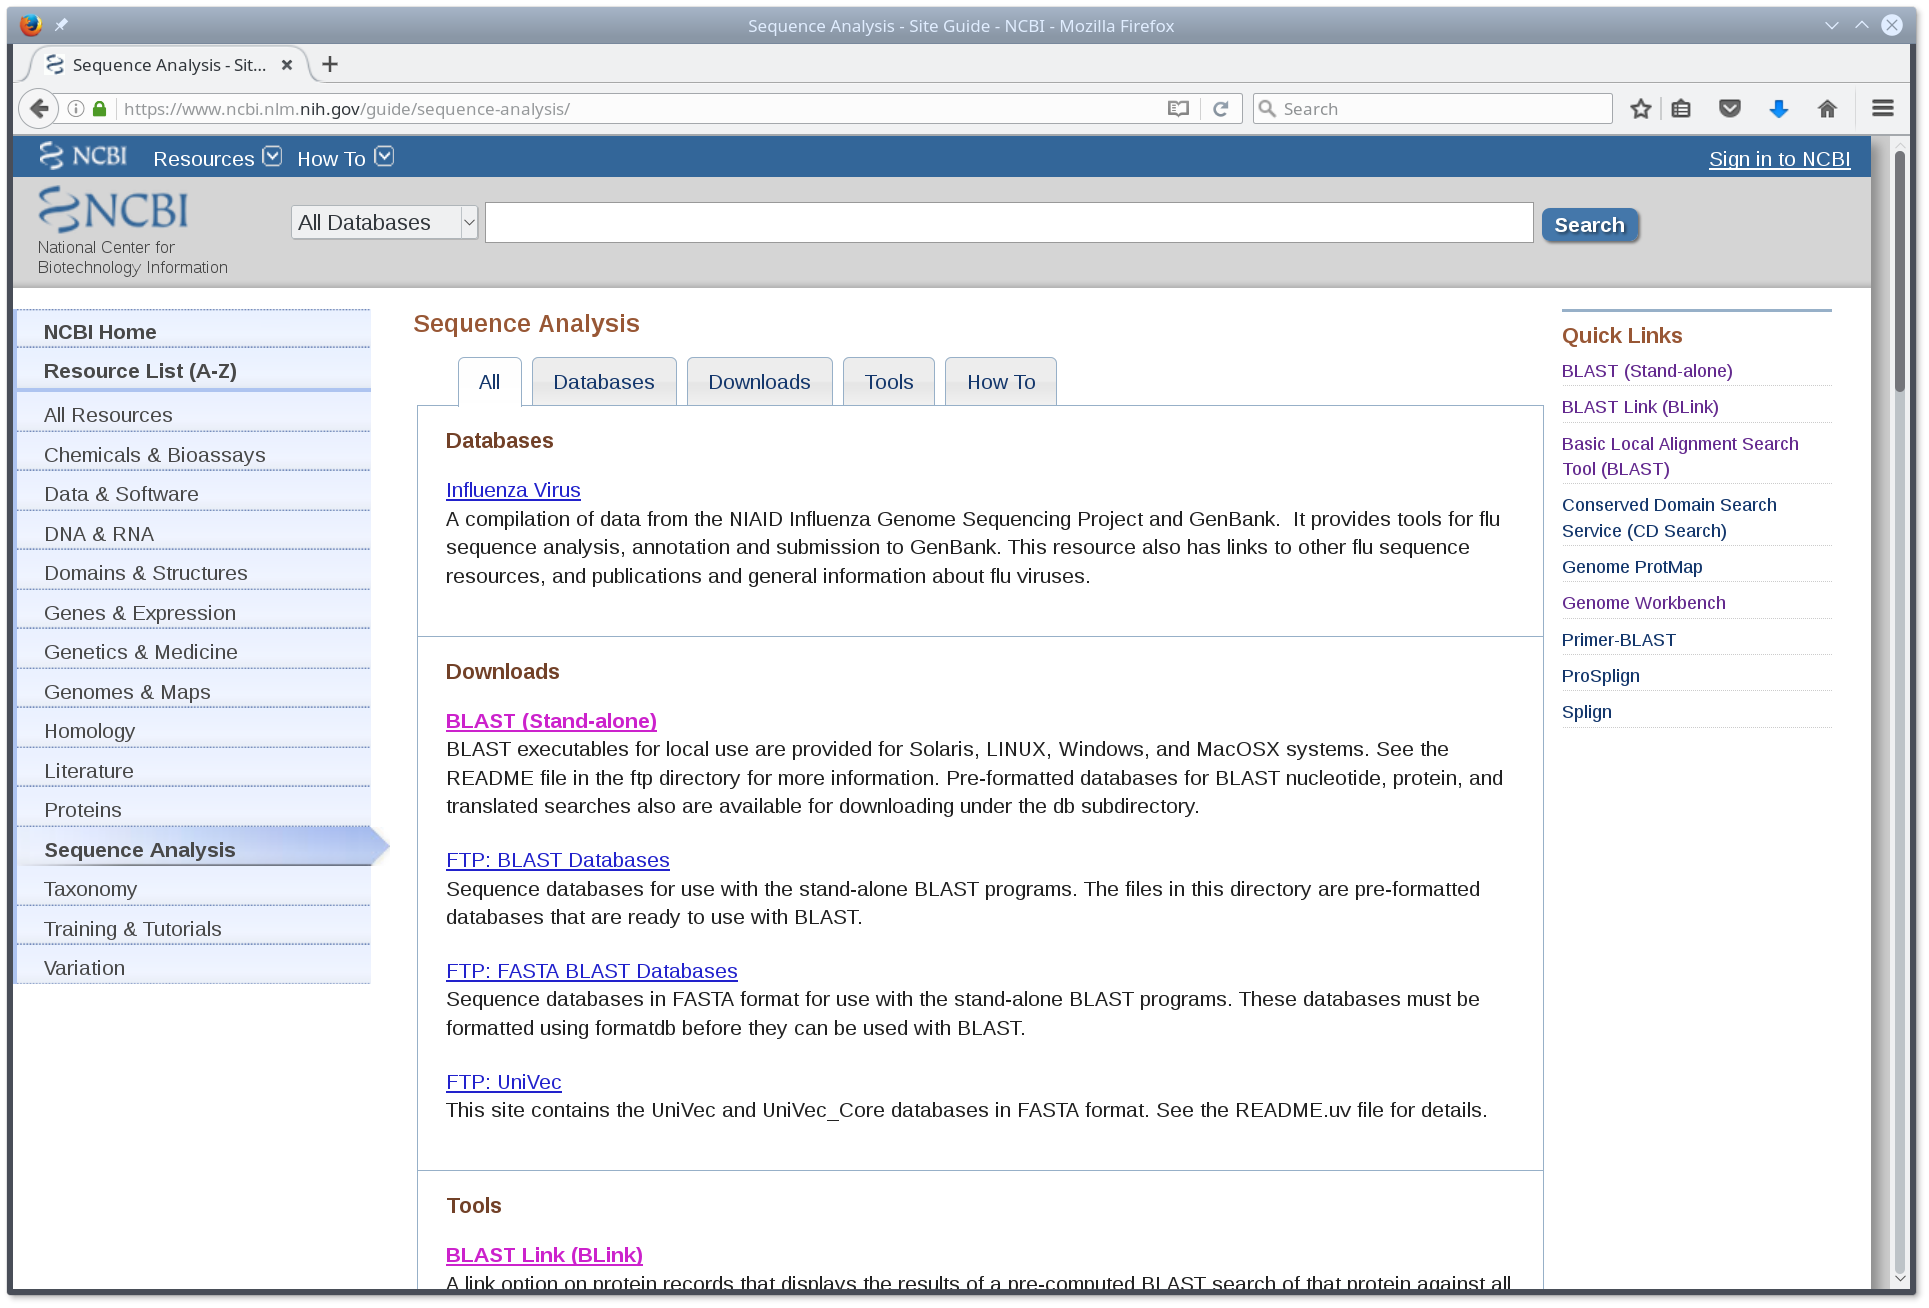
\includegraphics[width=0.7\textwidth]{images/ncbi_tools}
  \end{figure}
\end{frame}

\begin{frame}{EBI tools}
  \url{http://www.ebi.ac.uk/services}
  \begin{figure}[ht]
    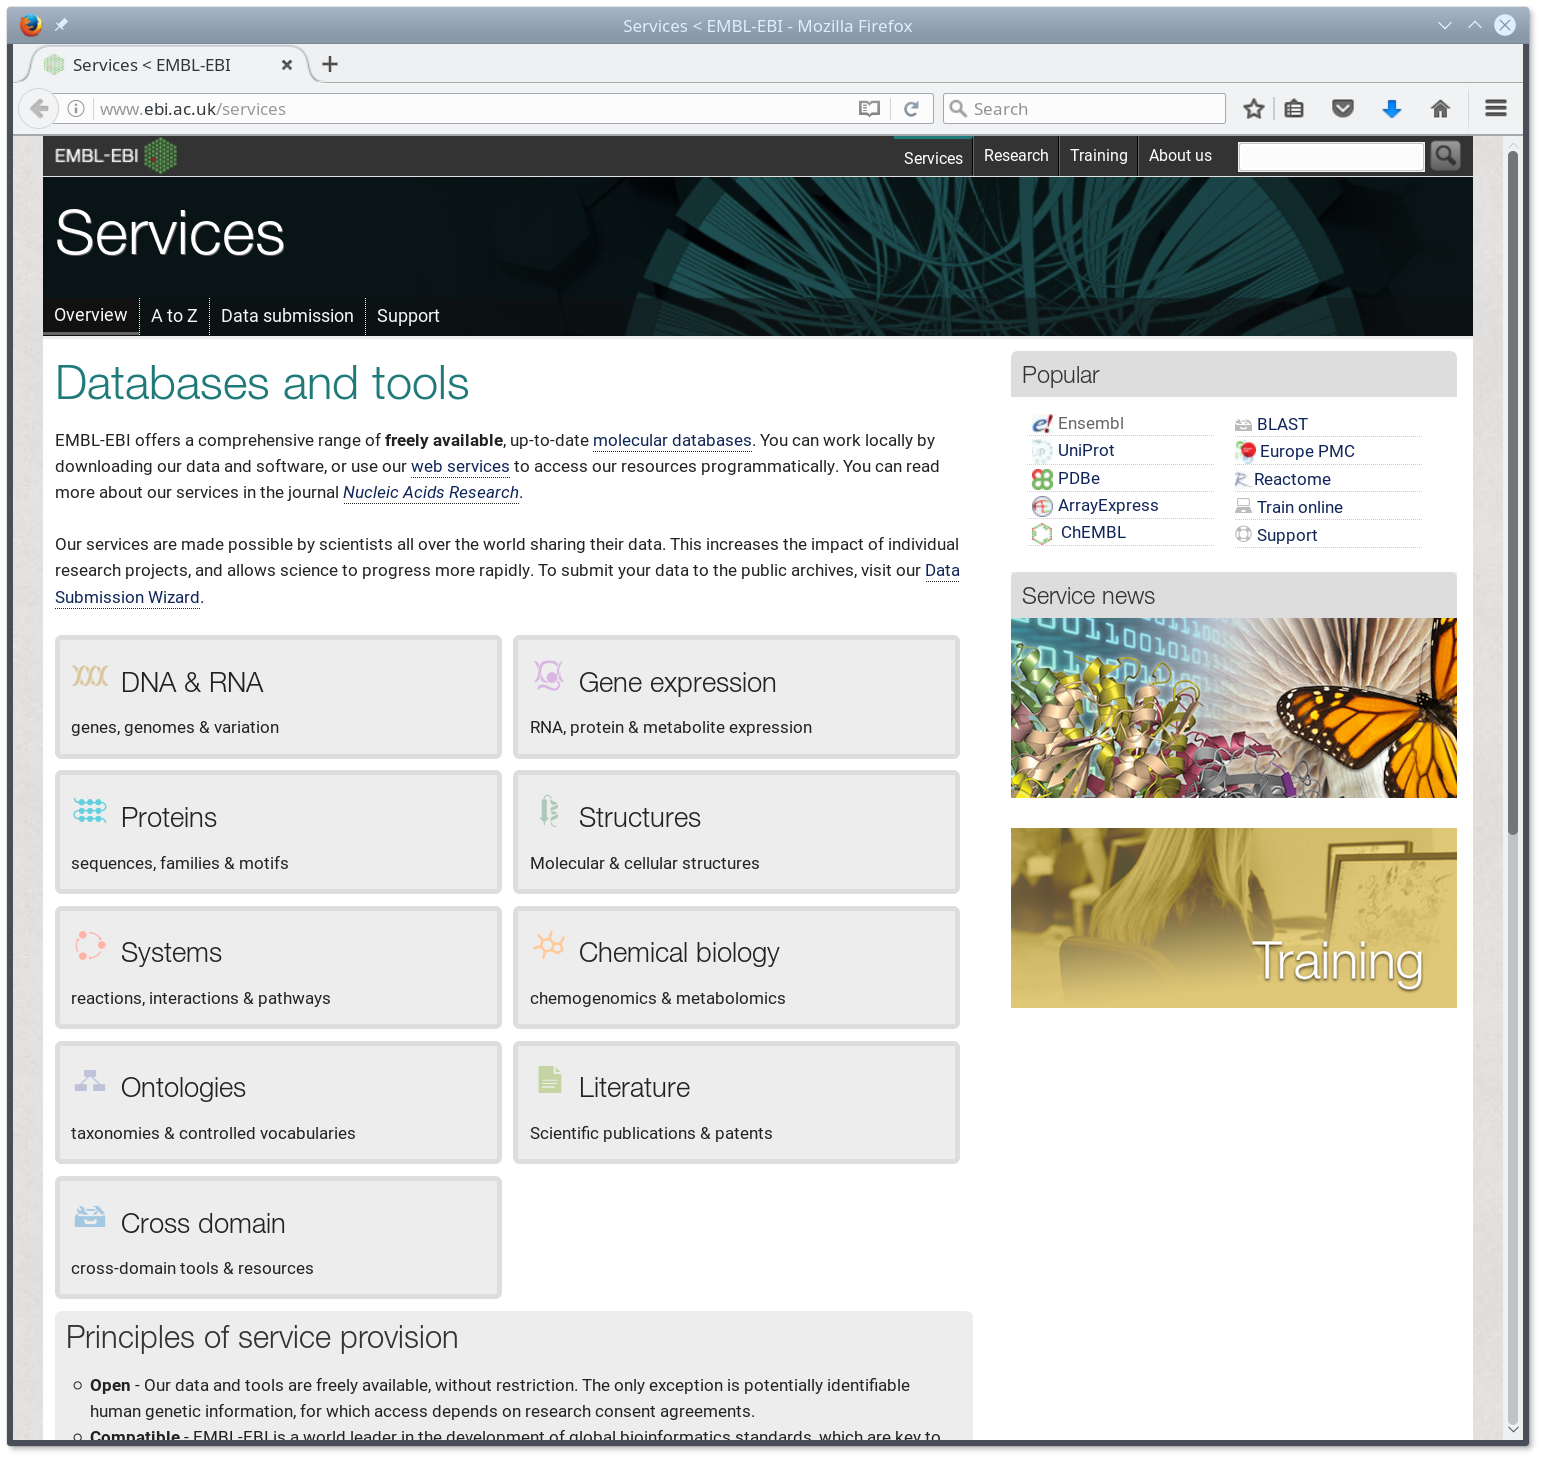
\includegraphics[width=0.7\textwidth]{images/ebi_tools1}
  \end{figure}
\end{frame}

\begin{frame}{ExPASy links}
  diverse collection of online tools:
  \url{http://www.expasy.org/genomics/sequence_alignment}
  \begin{figure}[ht]
    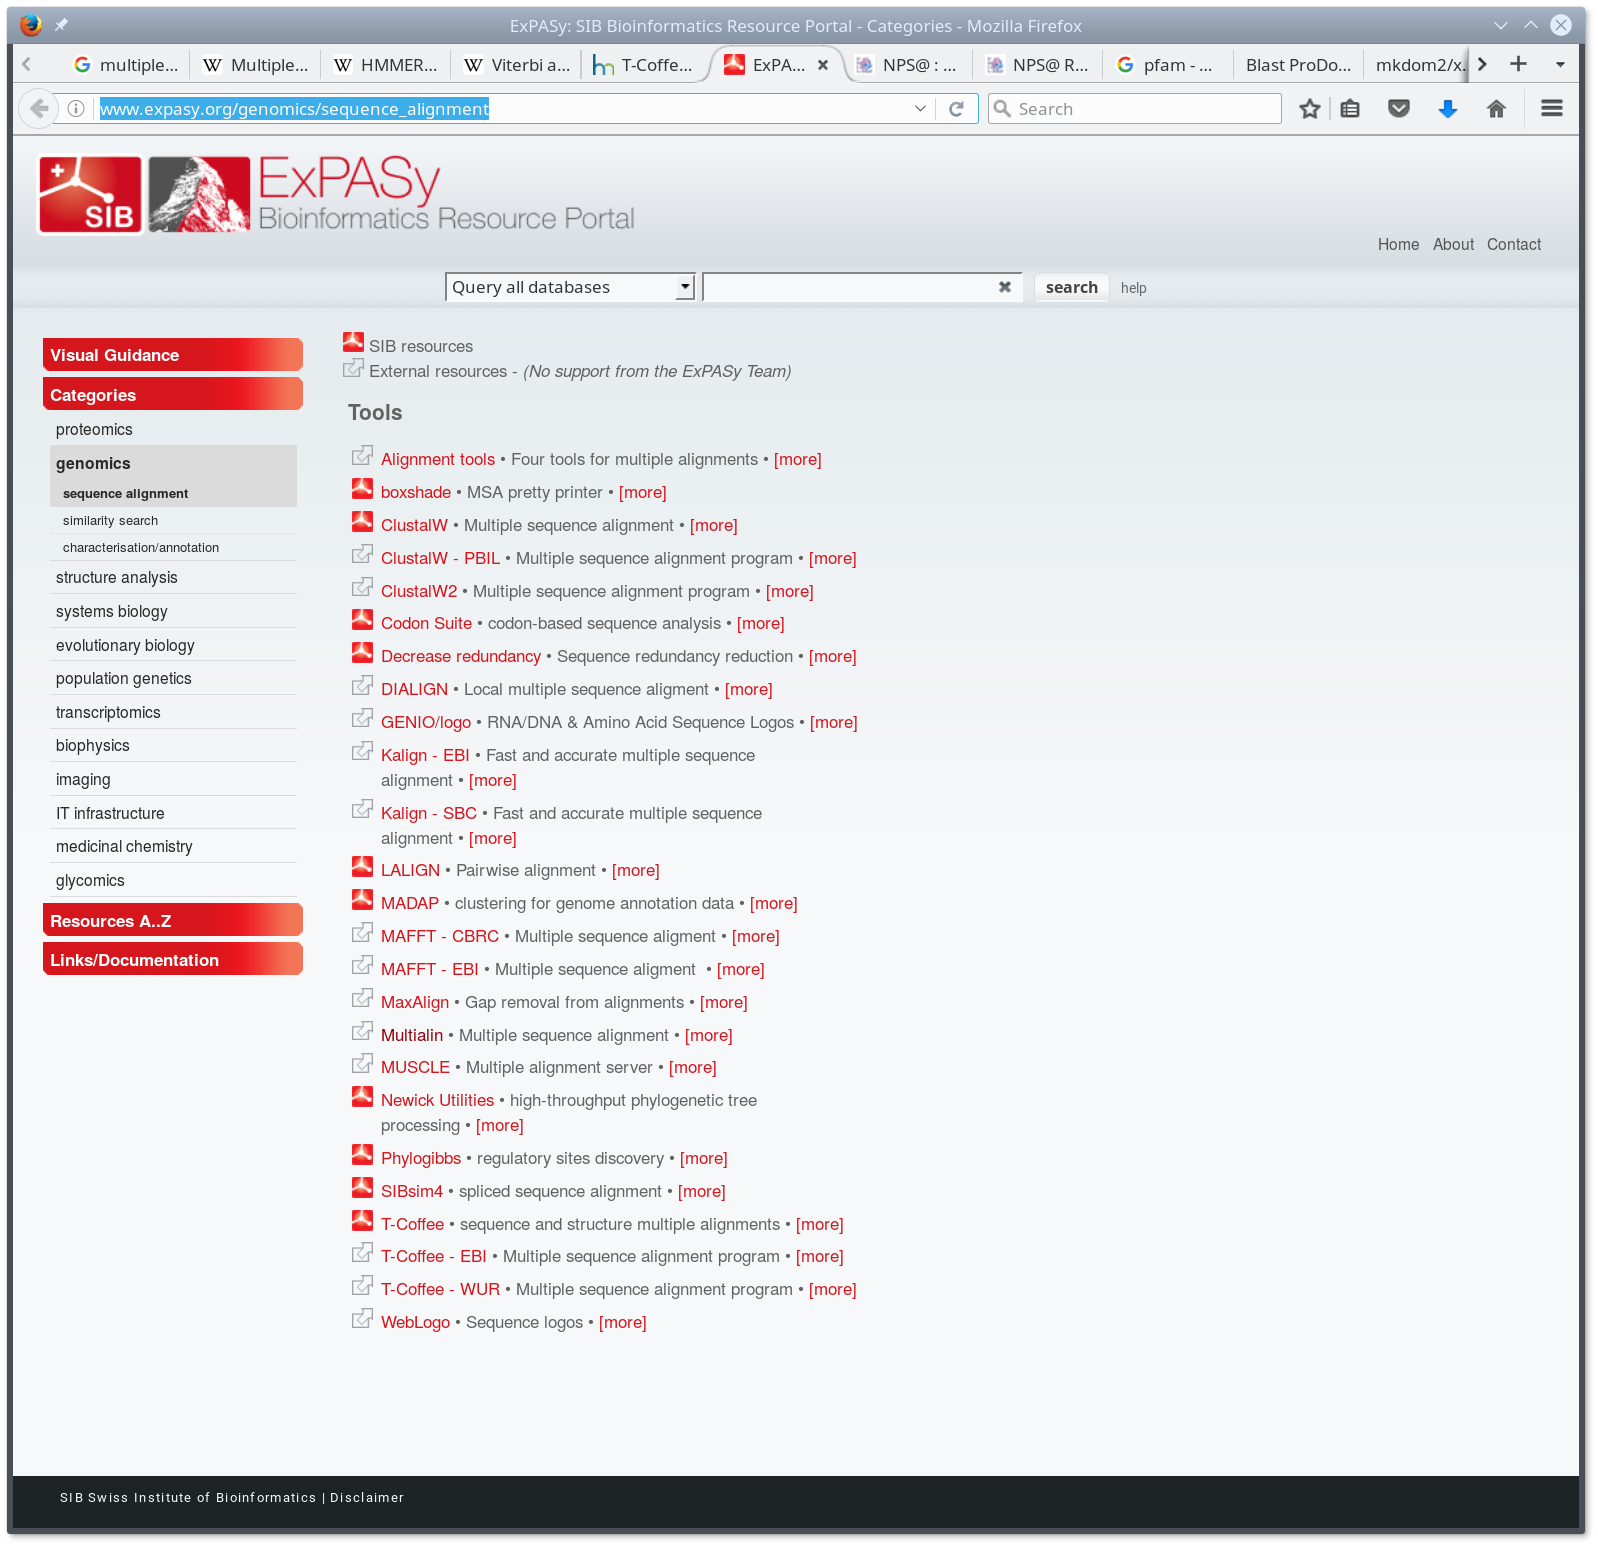
\includegraphics[width=0.7\textwidth]{images/expasy_tools}
  \end{figure}
\end{frame}

\begin{frame}{TCOFFEE}
  \url{http://tcoffee.crg.cat/apps/tcoffee/index.html}
  \begin{figure}[ht]
    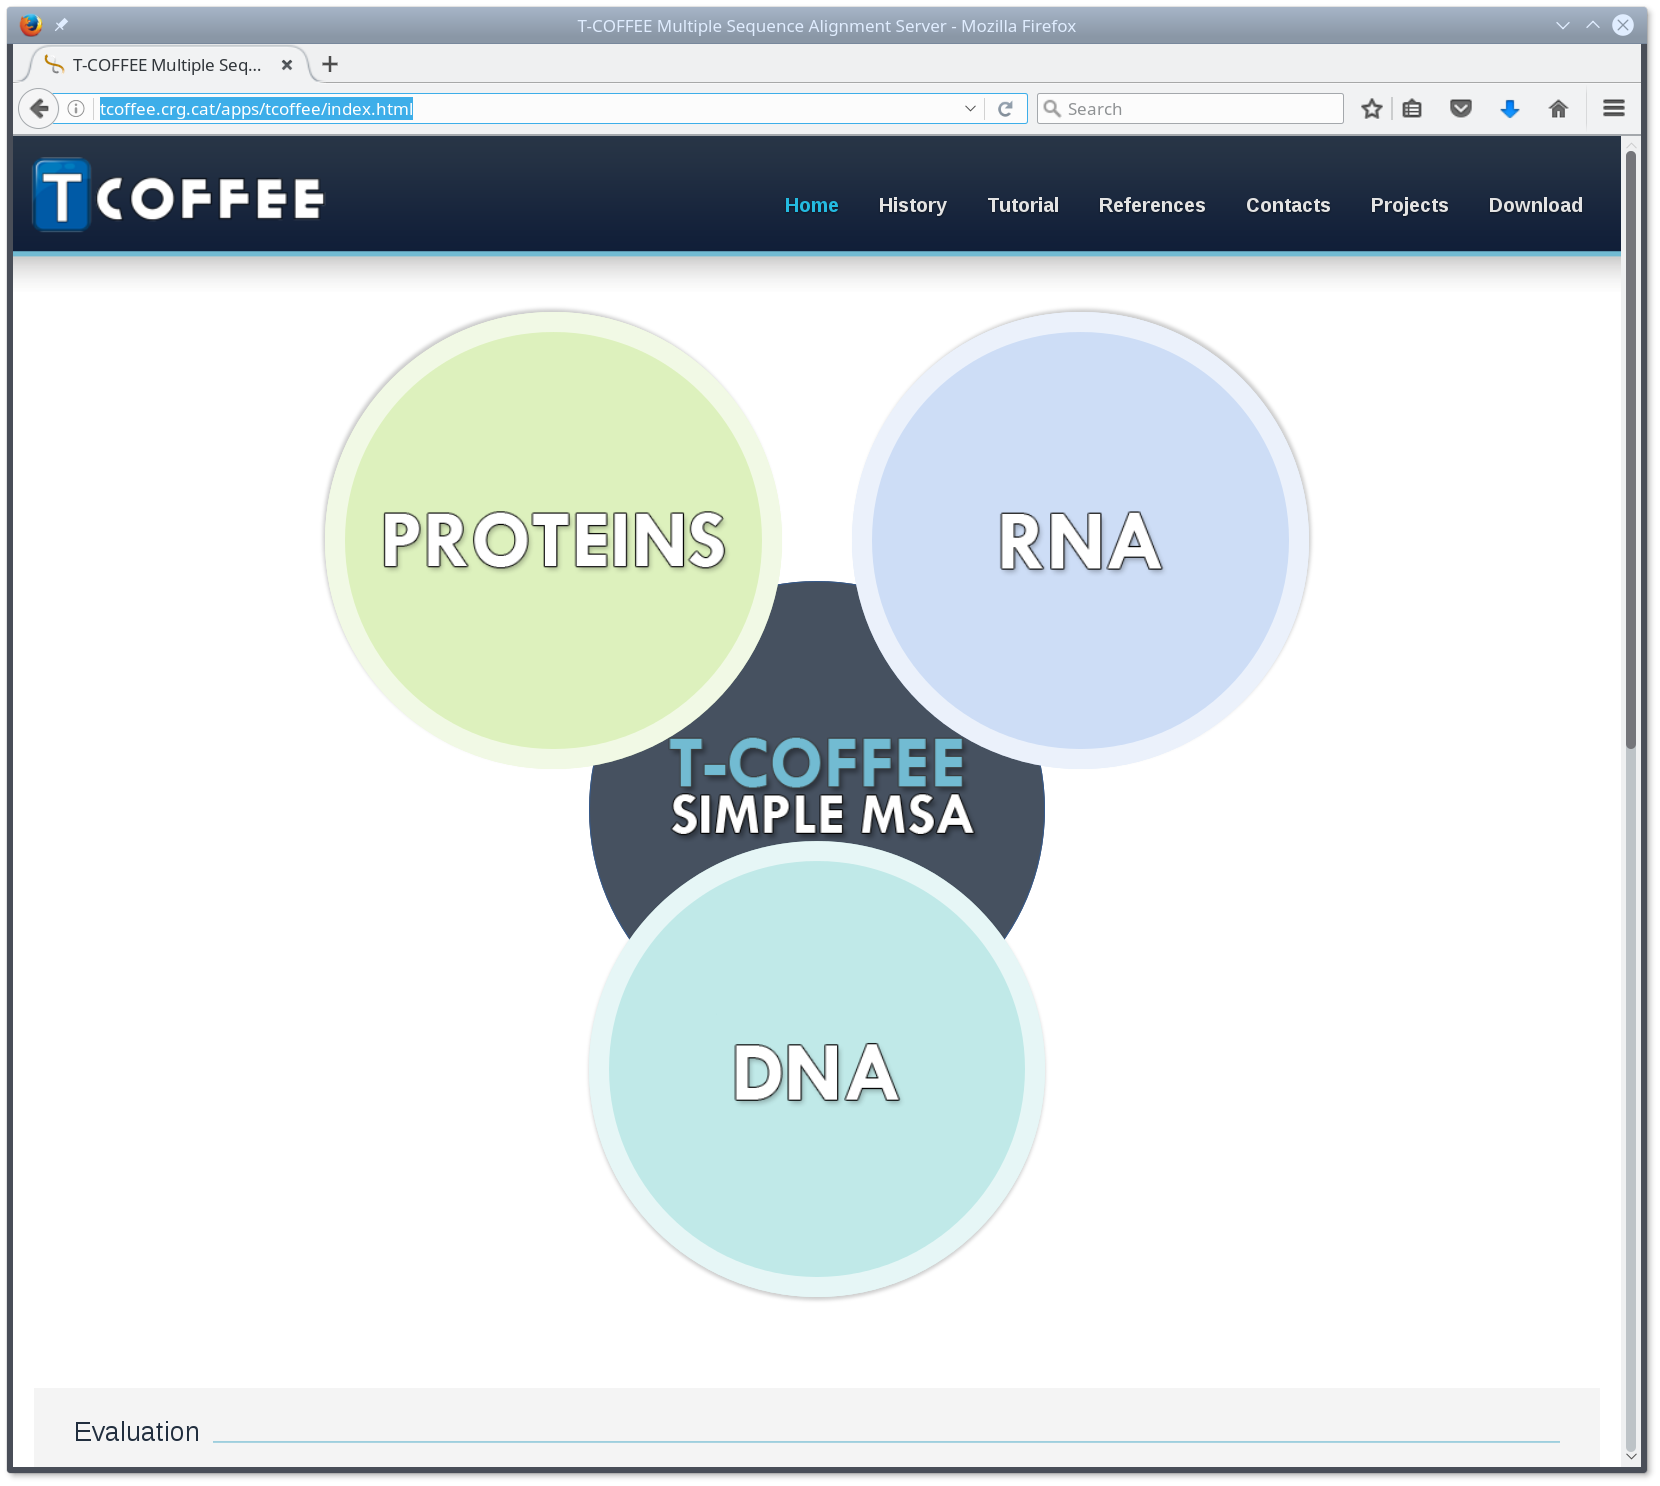
\includegraphics[width=0.7\textwidth]{images/tcoffee}
  \end{figure}
\end{frame}

\begin{frame}{Pairwise alignment}
  \begin{enumerate}
  \item Get some sequences (eg. NCBI)\\
    \url{http://www.ncbi.nlm.nih.gov/}
  \item Align some pairs at EBI\\
    EMBOSS \url{http://www.ebi.ac.uk/Tools/emboss/}
  \end{enumerate}

  or the other way around
\end{frame}

\begin{frame}{Get some sequences}
  \begin{enumerate}
  \item Search for 'nanog' or some other protein
  \item Choose Protein from the Proteins section :\\
    769 hits.
  \end{enumerate}
  \begin{figure}[ht]
    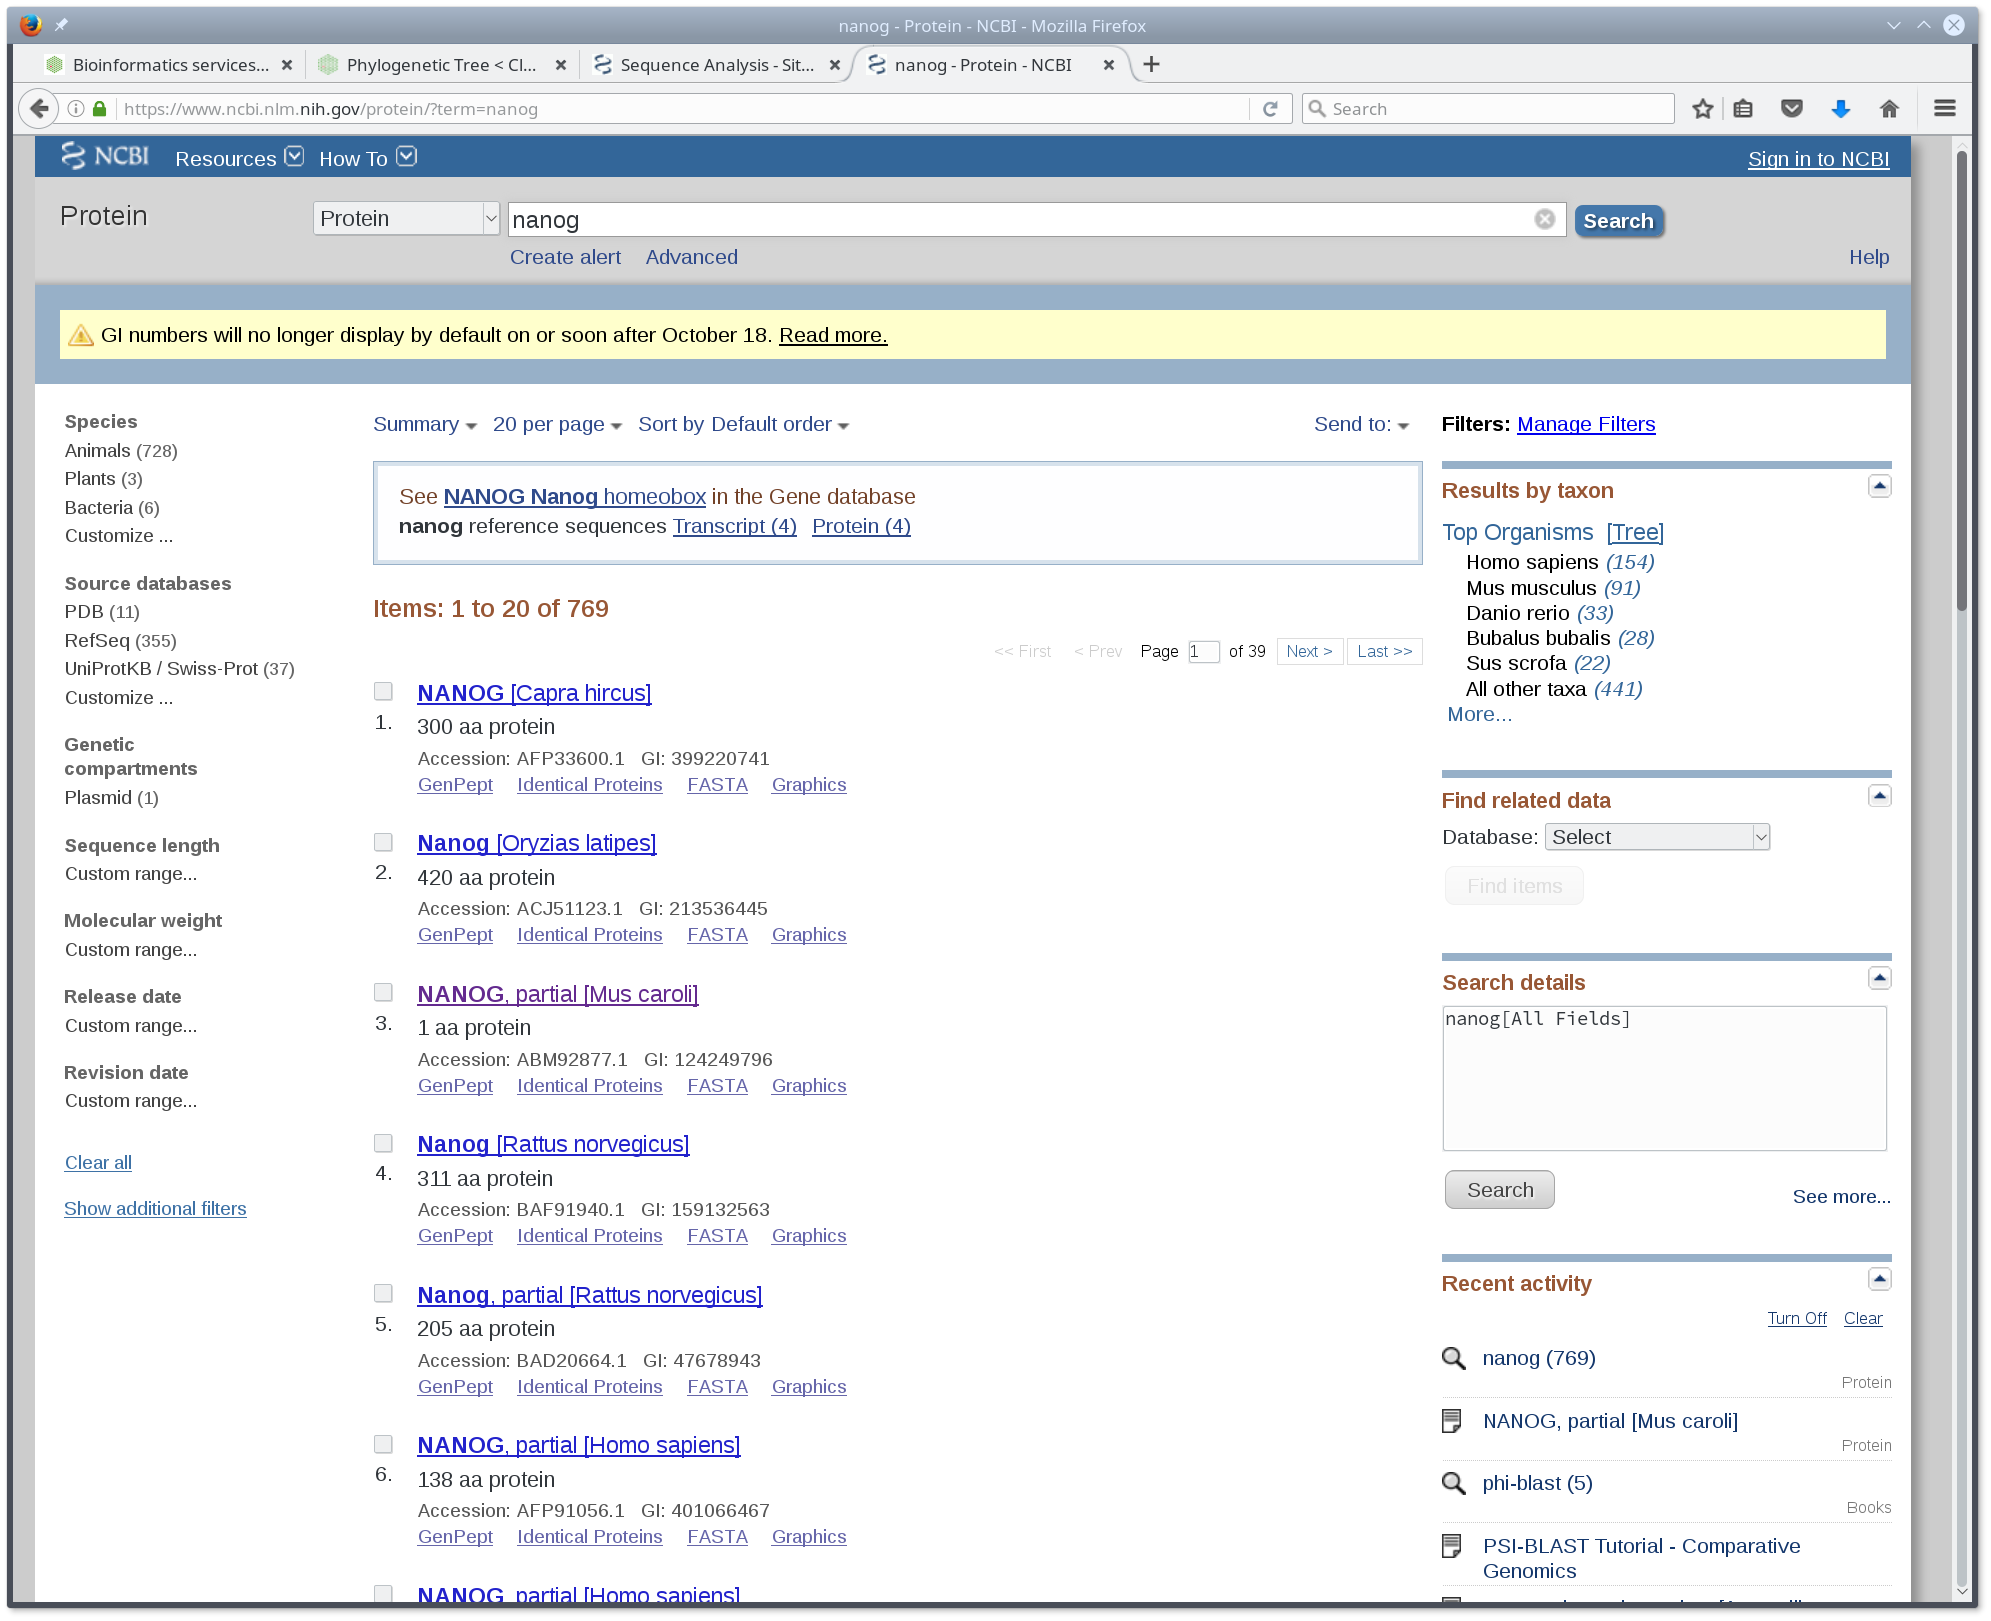
\includegraphics[width=0.7\textwidth]{images/ncbi_nanog_search_1.png}
  \end{figure}
\end{frame}

\begin{frame}{Get some sequences (2)}
  \begin{enumerate}
  \item Remove partial sequences: 'nanog NOT partial'\\
    514 sequences. Not bad:
  \item Select the ones you want:
  \end{enumerate}
  \begin{figure}[ht]
    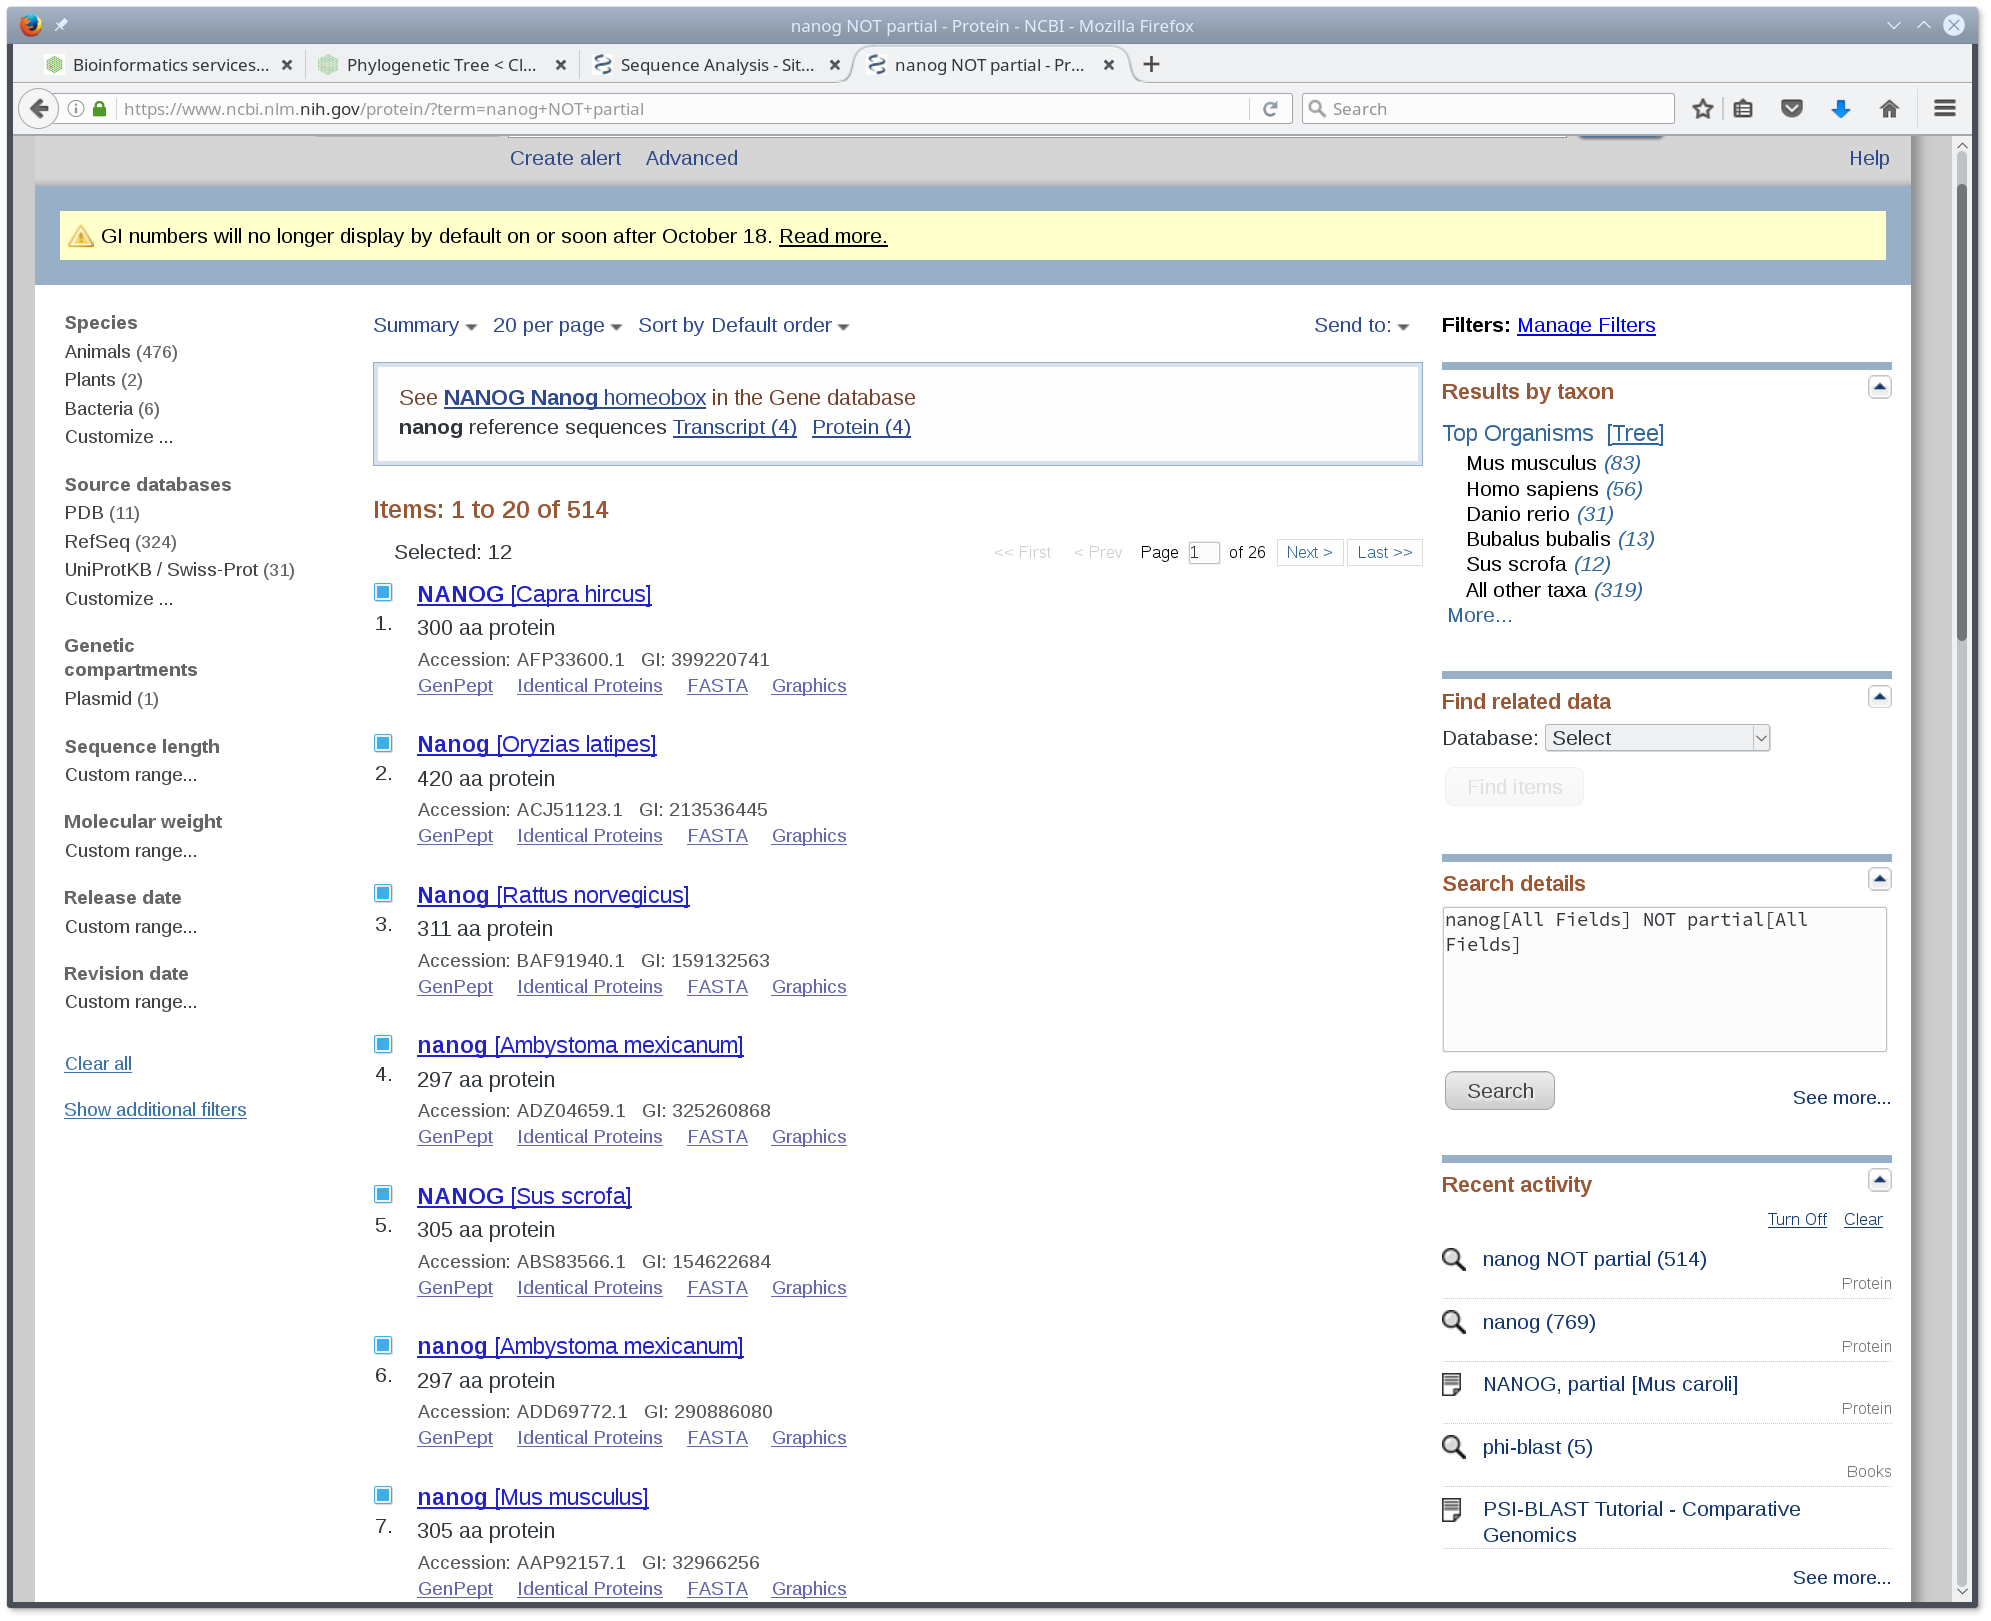
\includegraphics[width=0.7\textwidth]{images/ncbi_nanog_search_2}
  \end{figure}
\end{frame}

\begin{frame}{Get sequence file}
  click the little send to button and save as a file:
  \begin{figure}[ht]
    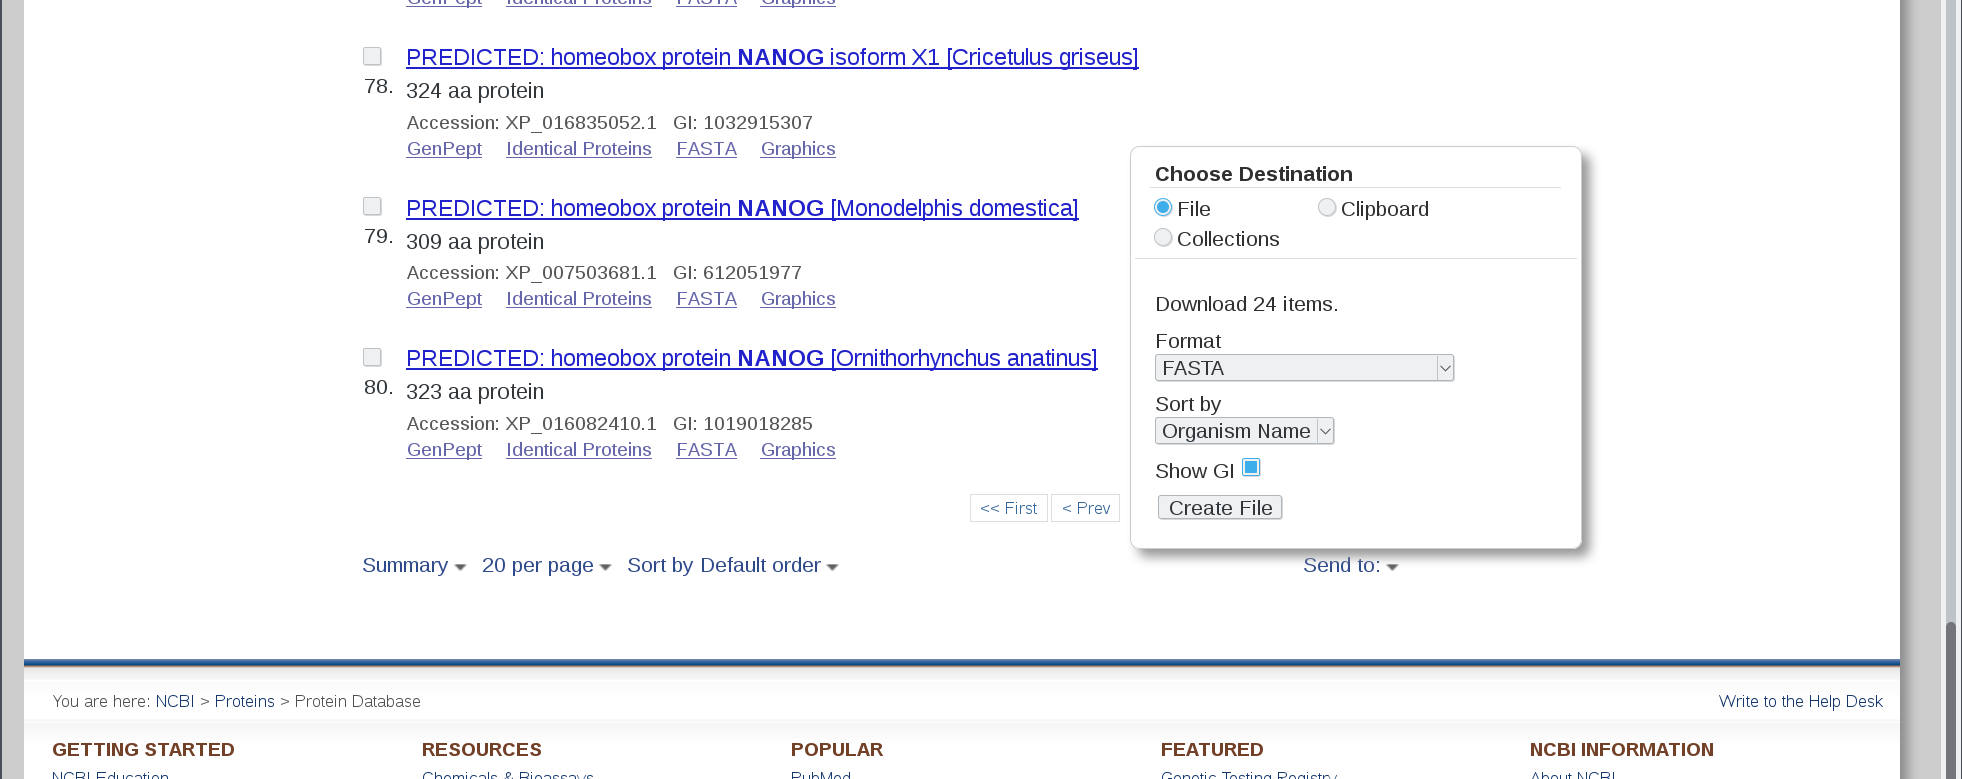
\includegraphics[width=0.7\textwidth]{images/ncbi_nanog_send_to}
  \end{figure}
\end{frame}

\begin{frame}{lots of nanogs}
  We got a whole load of sequences:
  \begin{figure}[ht]
    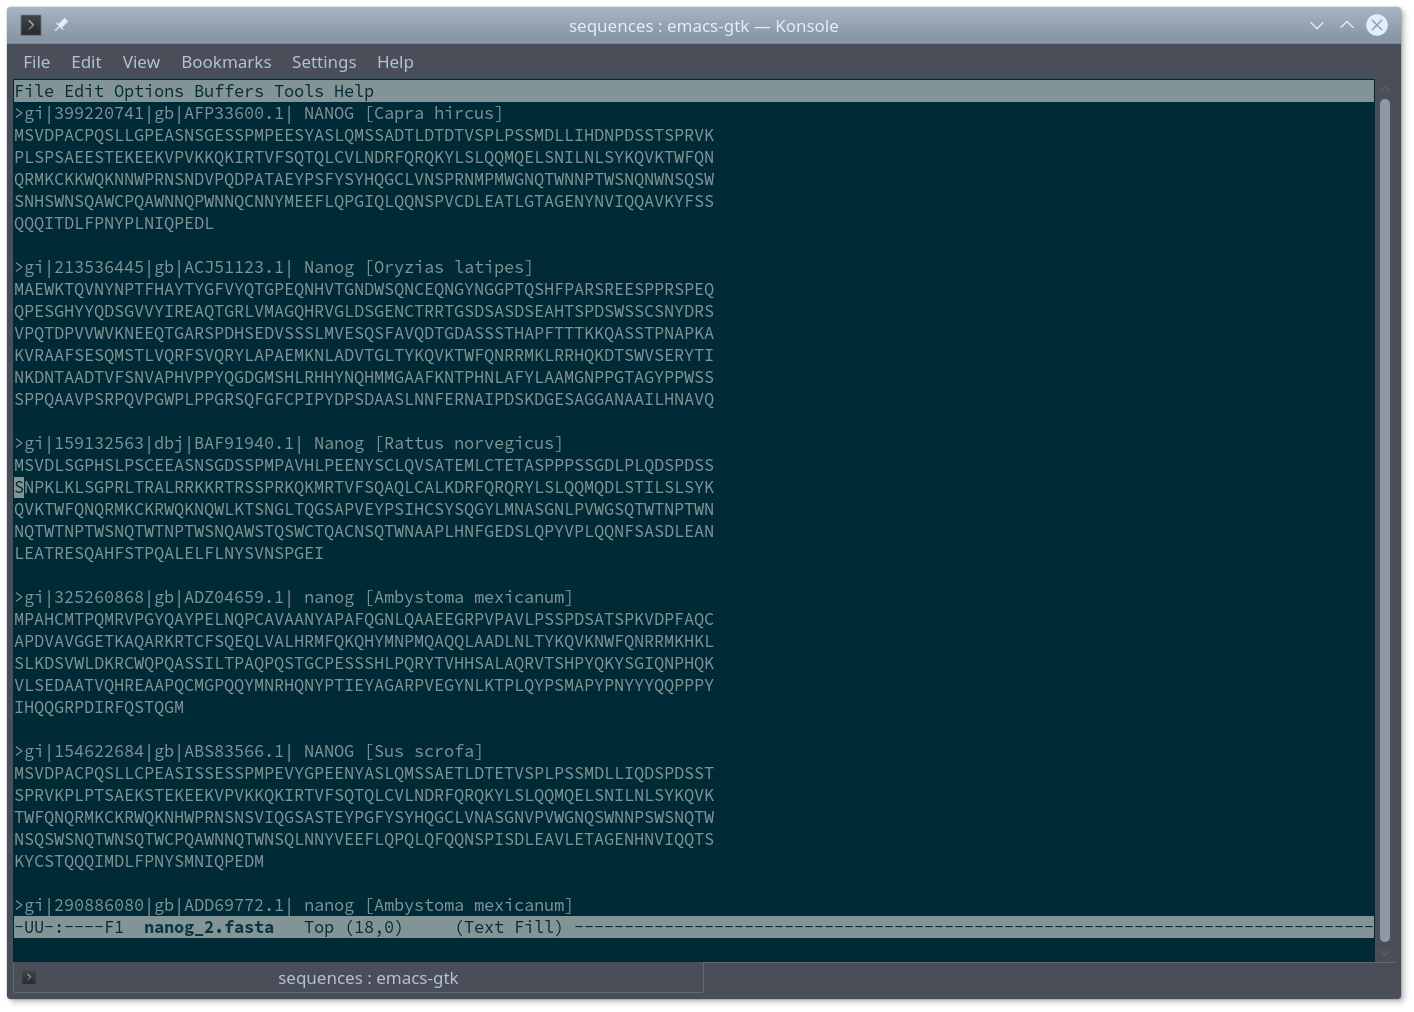
\includegraphics[width=0.7\textwidth]{images/nanog_multiple_fasta}
  \end{figure}
\end{frame}

\begin{frame}[fragile]{how many sequence}
  \begin{consolecode}
    > grep -c '>' nanog_2.fasta 
    24
  \end{consolecode}
  
  From how many species?
  \begin{consolecode}
    > grep -Po '\[.+\]' nanog_2.fasta | sort
    [Ambystoma mexicanum]
    [Ambystoma mexicanum]
    [Anas platyrhynchos]
    [Bos taurus]
    [Bubalus bubalis]
    [Callithrix jacchus]
    [Capra hircus]
    [Capra hircus]
    [Capra hircus]
    [Danio rerio]
    [Felis catus]
    [Gallus gallus]
    [Homo sapiens]
    [Macaca fascicularis]
    [Manis javanica]
    [Microtus levis]
    [Mus musculus]
    [Oryzias latipes]
    [Oryzias latipes]
    [Pan troglodytes]
    [Pan troglodytes]
    [Papio anubis]
    [Rattus norvegicus]
    [Sus scrofa]
  \end{consolecode}
\end{frame}

\begin{frame}[fragile]{so how many species?}
  \begin{consolecode}
    > grep -Po '\[.+\]' nanog_2.fasta | sort -u | wc
     19      38     324
  \end{consolecode}
  
  are they unique sequences. Look at the identifiers:
  \begin{consolecode}
    > grep -Po '>gi\|\d+' nanog_2.fasta | sort -u | wc
     24      24     334
  \end{consolecode}

  \pause
  To work out what is going on here:
  \begin{consolecode}
    > man grep
    > man sort
    > man wc
  \end{consolecode}

  This now even works on Windows (10) as it comes with an Ubuntu command line system!
\end{frame}

\begin{frame}[fragile]{$\rightarrow$ one sequence per species}
  \begin{perlcode}
    #!/usr/bin perl -w
    ## This reads the sequences from STDIN
    ## And prints to STDOUT
    $skip_seq = 0;
    %species = ();
    while(<>){
      if( $_ =~ /^>\S+\s+.+?\[(.+)\]$/){
        $skip_seq = defined( $species{$1} );
        $species{$1} = 1;
      }
      if(!$skip_seq){
        print;
      }
   }
  \end{perlcode}

  \begin{consolecode}
    > cat nanog_2.fasta | ./prune_species.pl | grep -c '>'
    19
  \end{consolecode}
  \small should work for all sequences from NCBI
  \blfootnote{OK, so the regular expression is a little bit complicated, but
    doesn't take that long to work it out.}
\end{frame}

\begin{frame}{Global alignment}
  \url{http://www.ebi.ac.uk/Tools/psa/emboss_needle/}
  \begin{figure}[ht]
    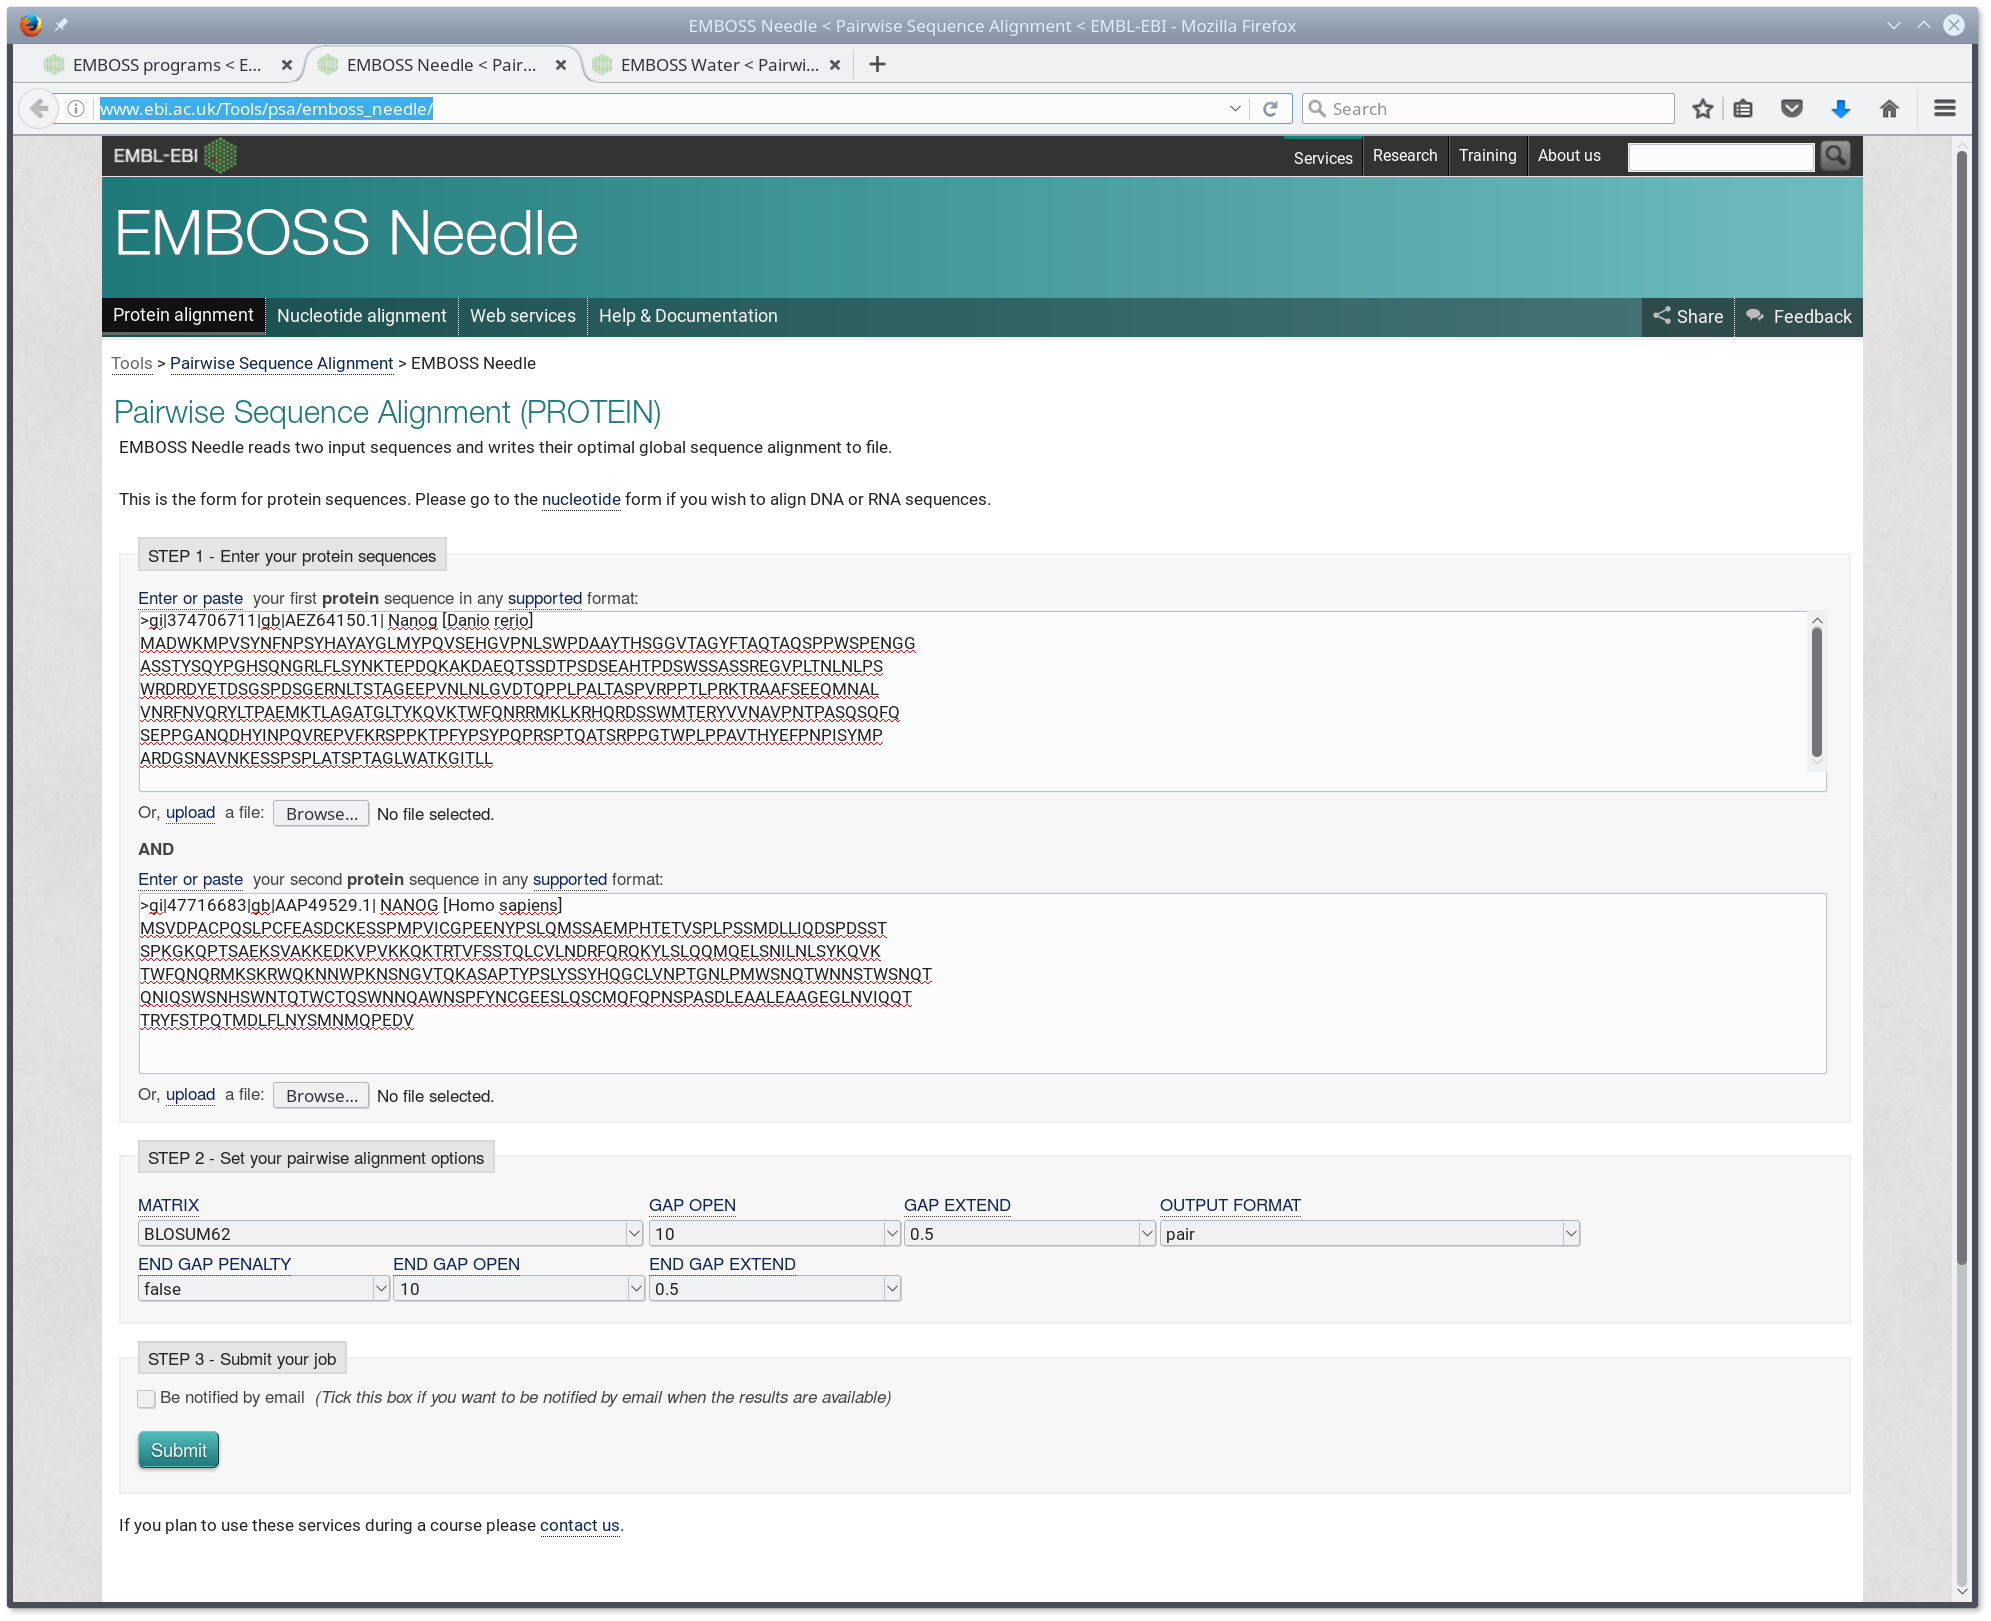
\includegraphics[width=0.7\textwidth]{images/emboss_needle}
  \end{figure}
  \tiny Copying and pasting until we get RSI...
\end{frame}

\begin{frame}{Global alignment (2)}
  \begin{figure}[ht]
    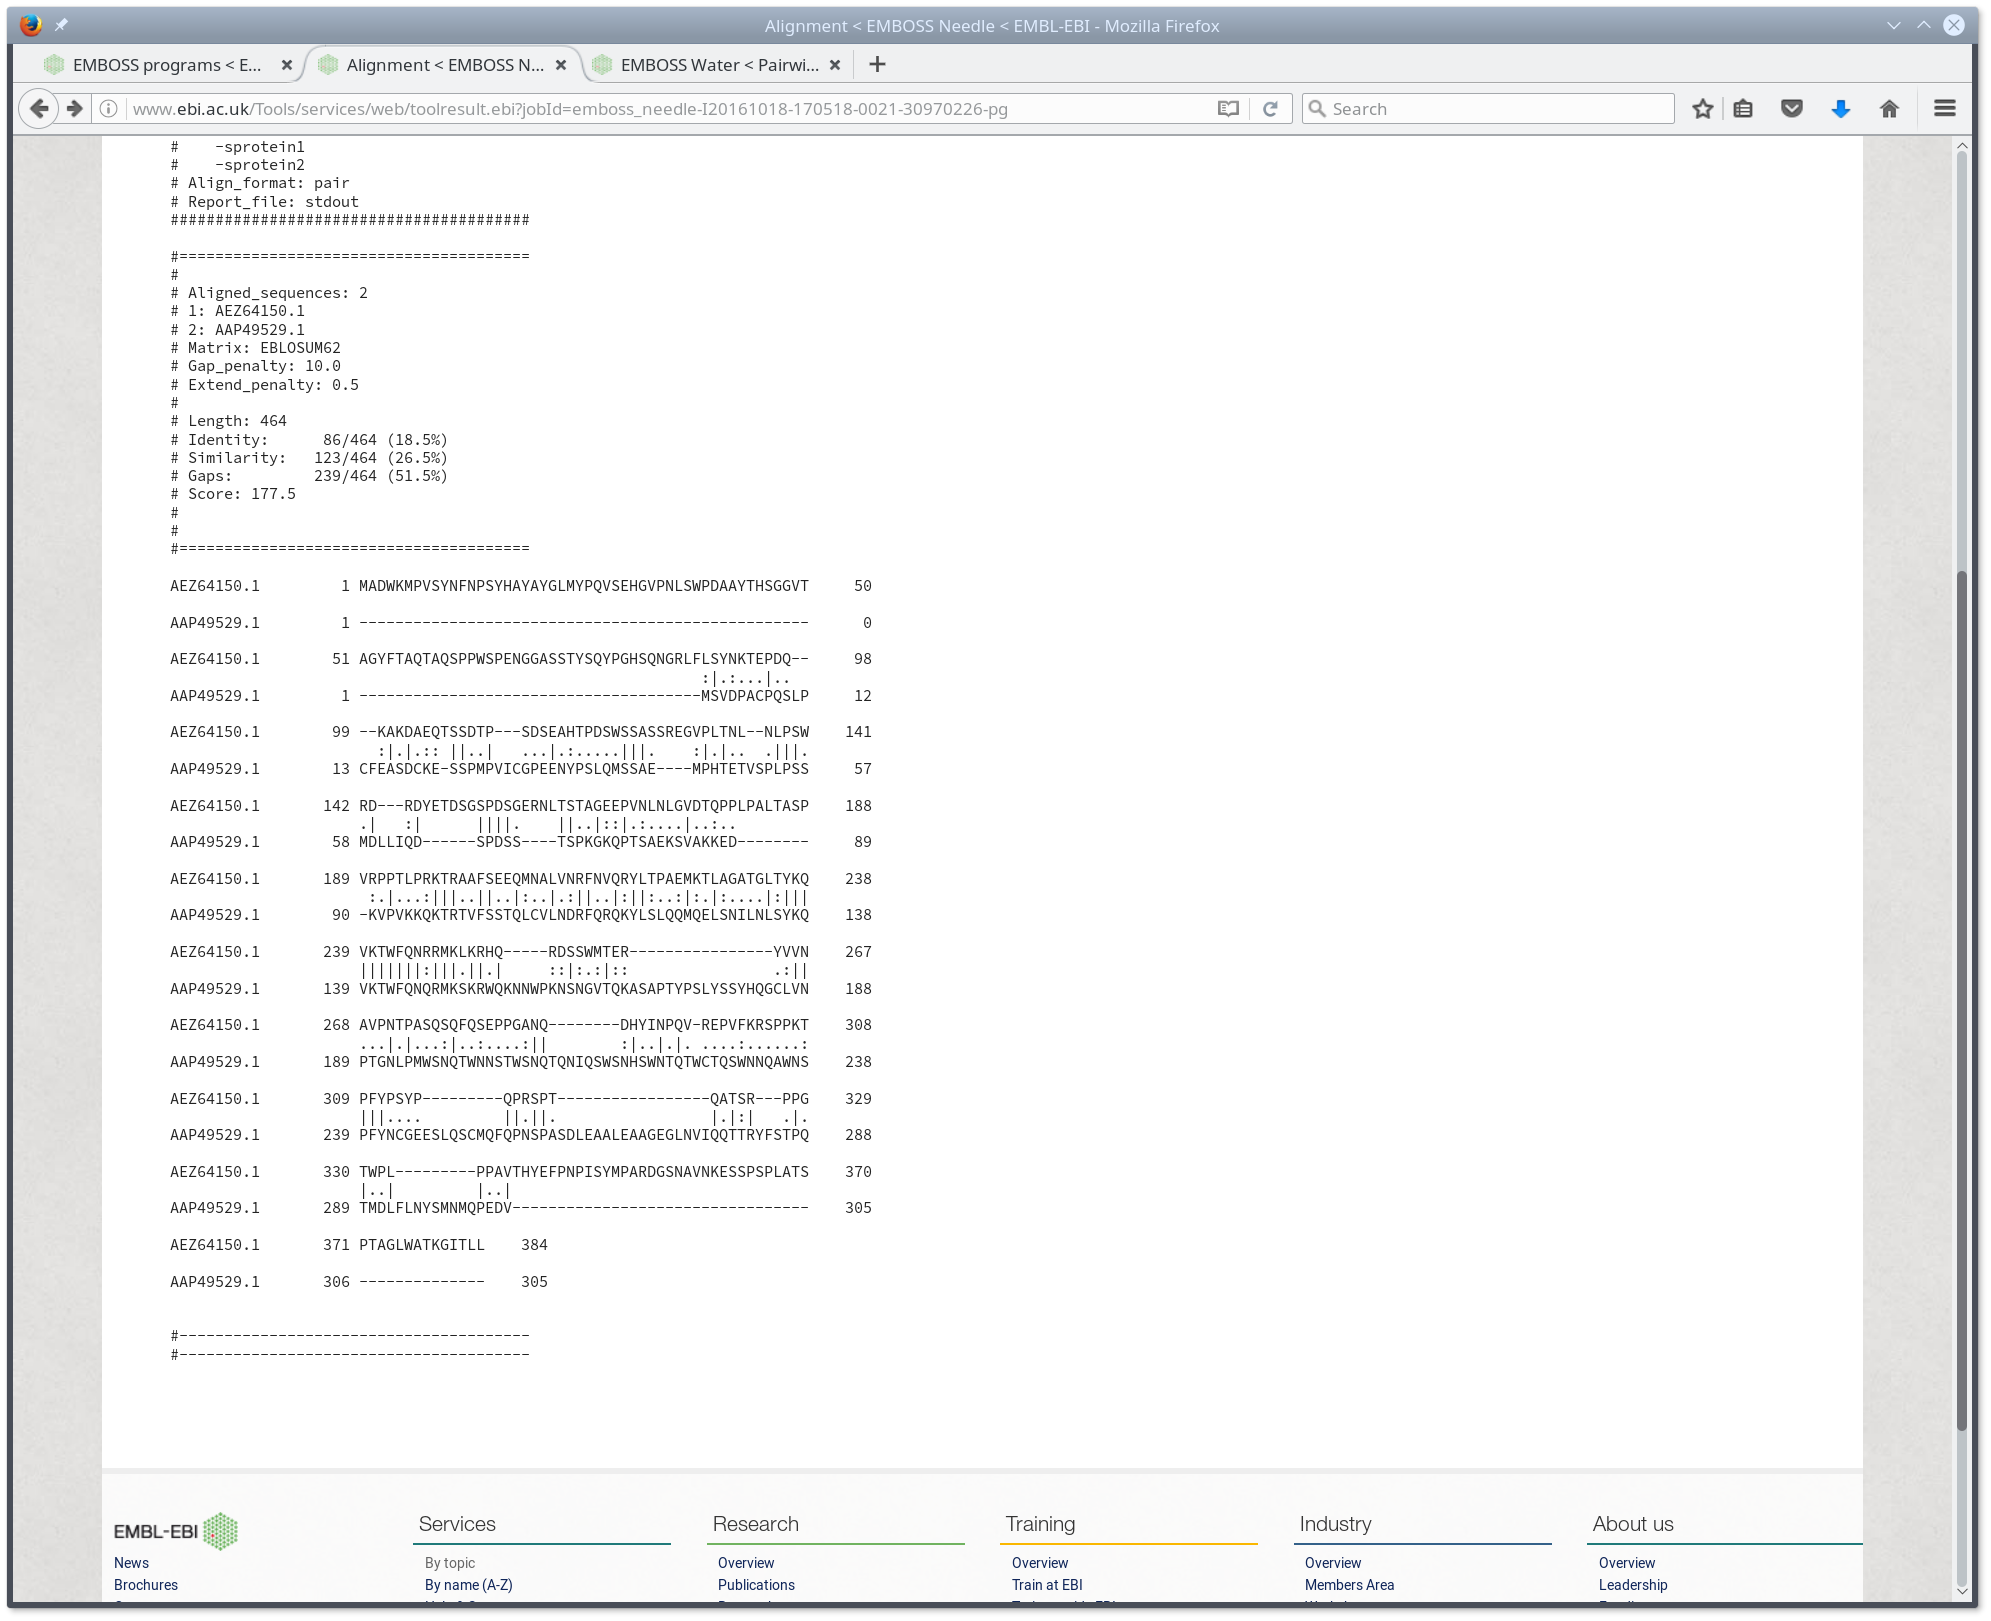
\includegraphics[width=0.9\textwidth]{images/emboss_needle_result}
  \end{figure}
\end{frame}

\begin{frame}{Local alignment}
  \url{http://www.ebi.ac.uk/Tools/psa/emboss_water/}
  \begin{figure}[ht]
    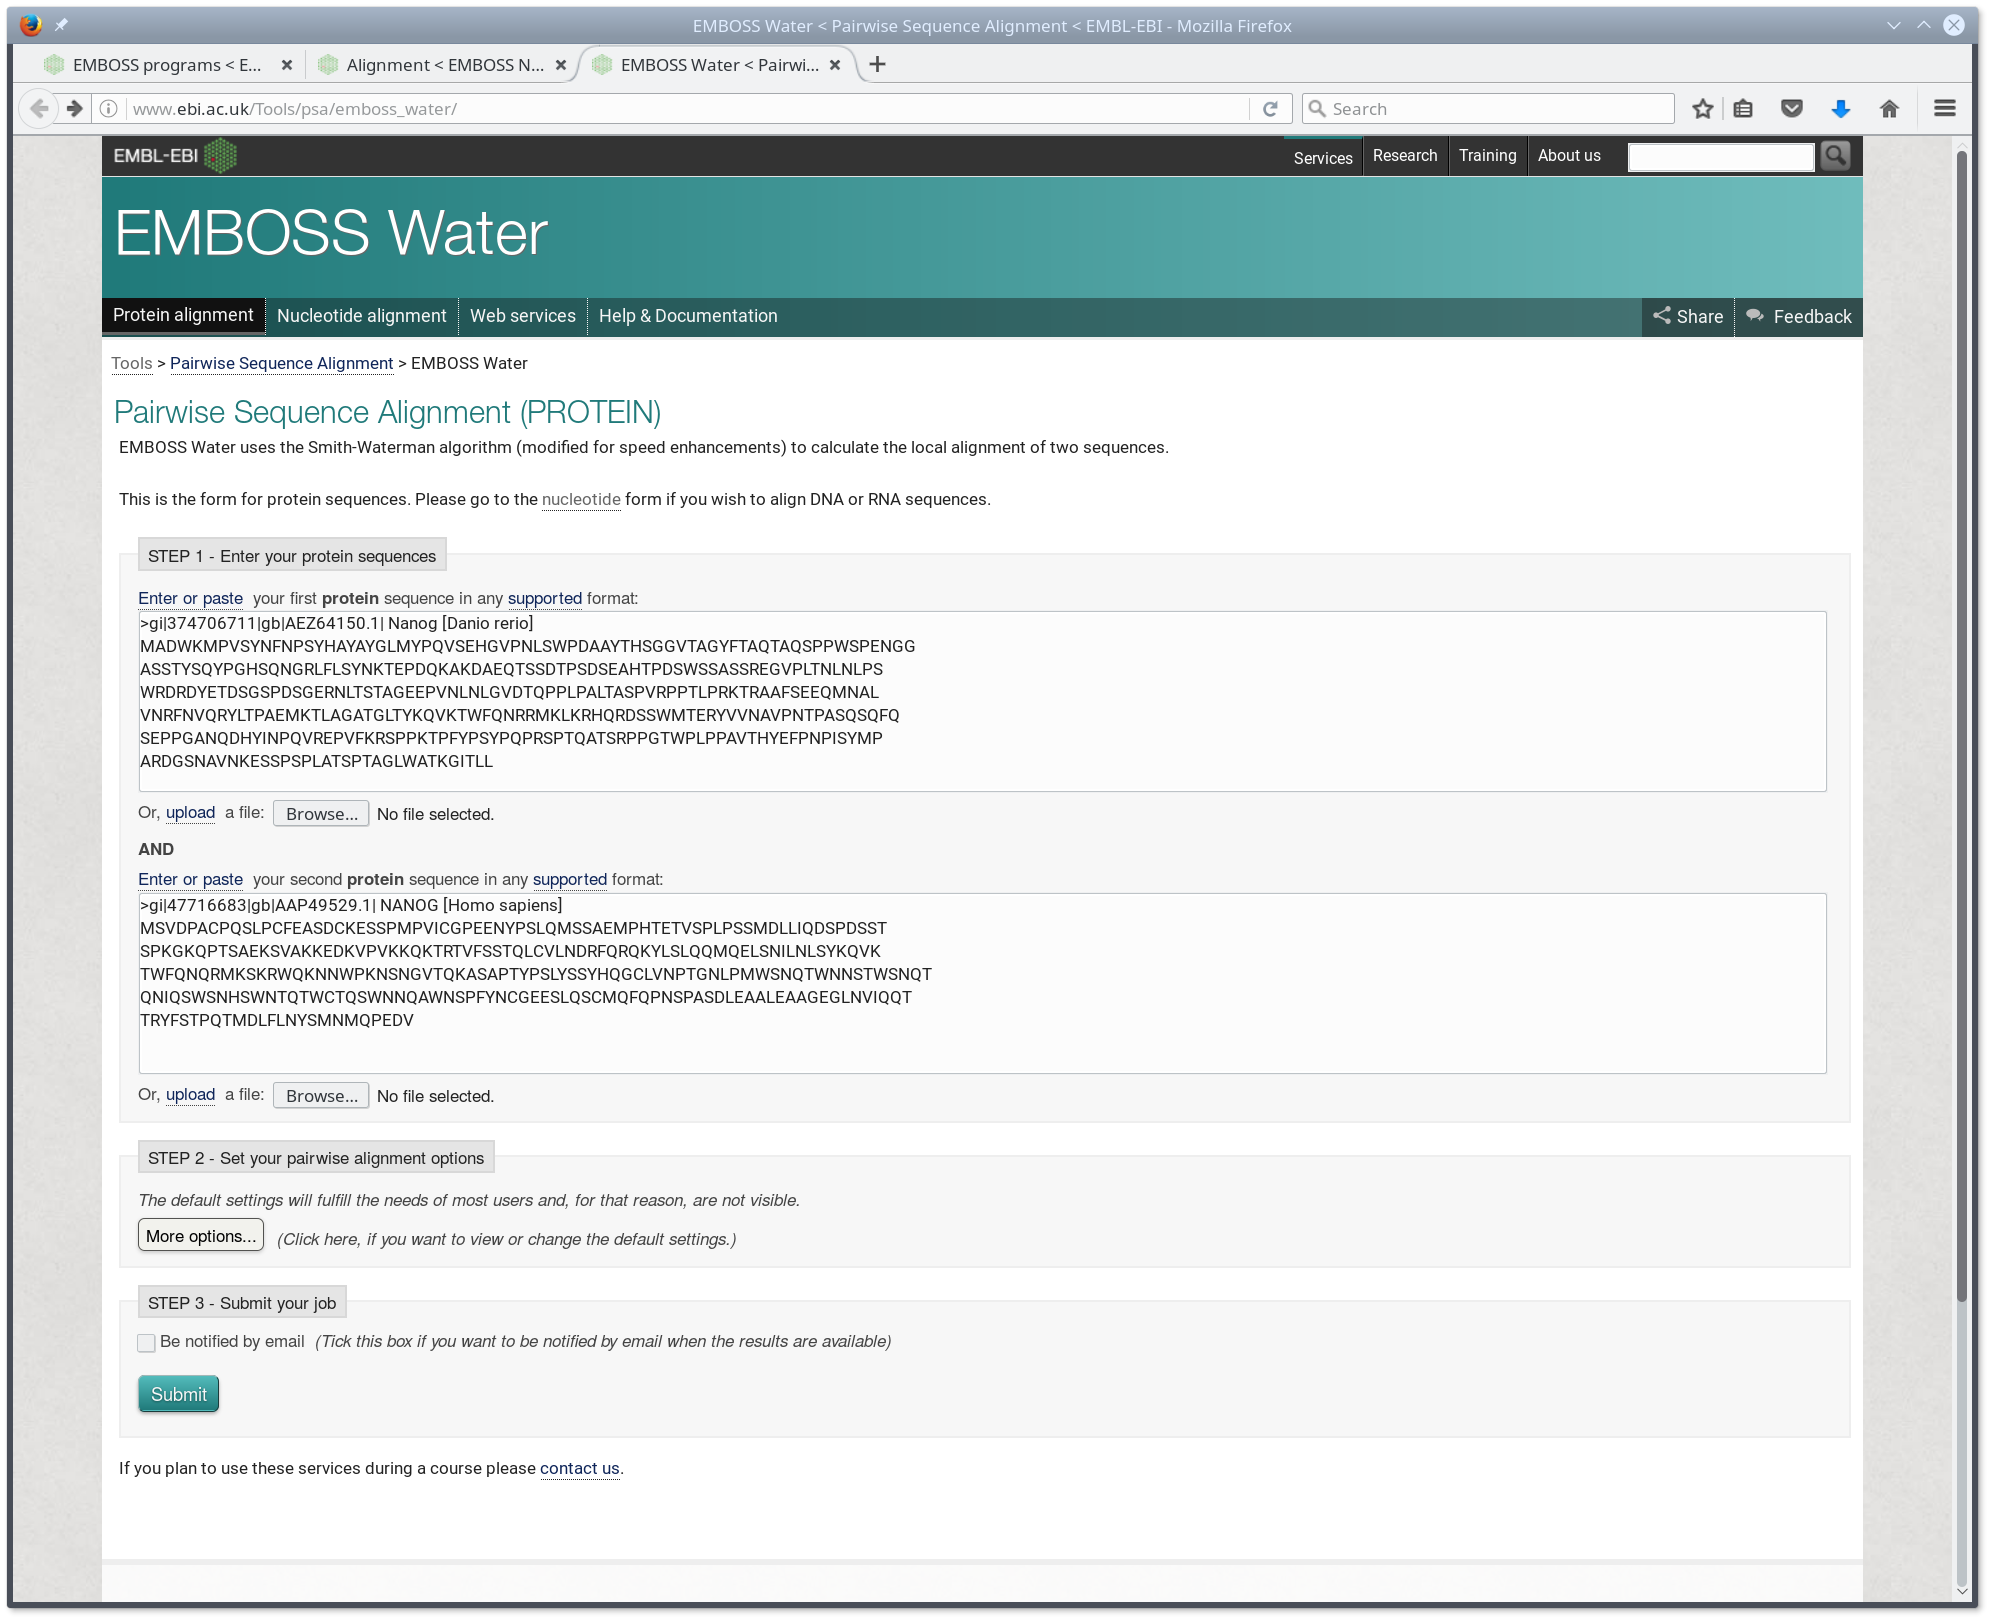
\includegraphics[width=0.7\textwidth]{images/emboss_water}
  \end{figure}
\end{frame}

\begin{frame}{Local alignment (2)}
  \begin{figure}[ht]
    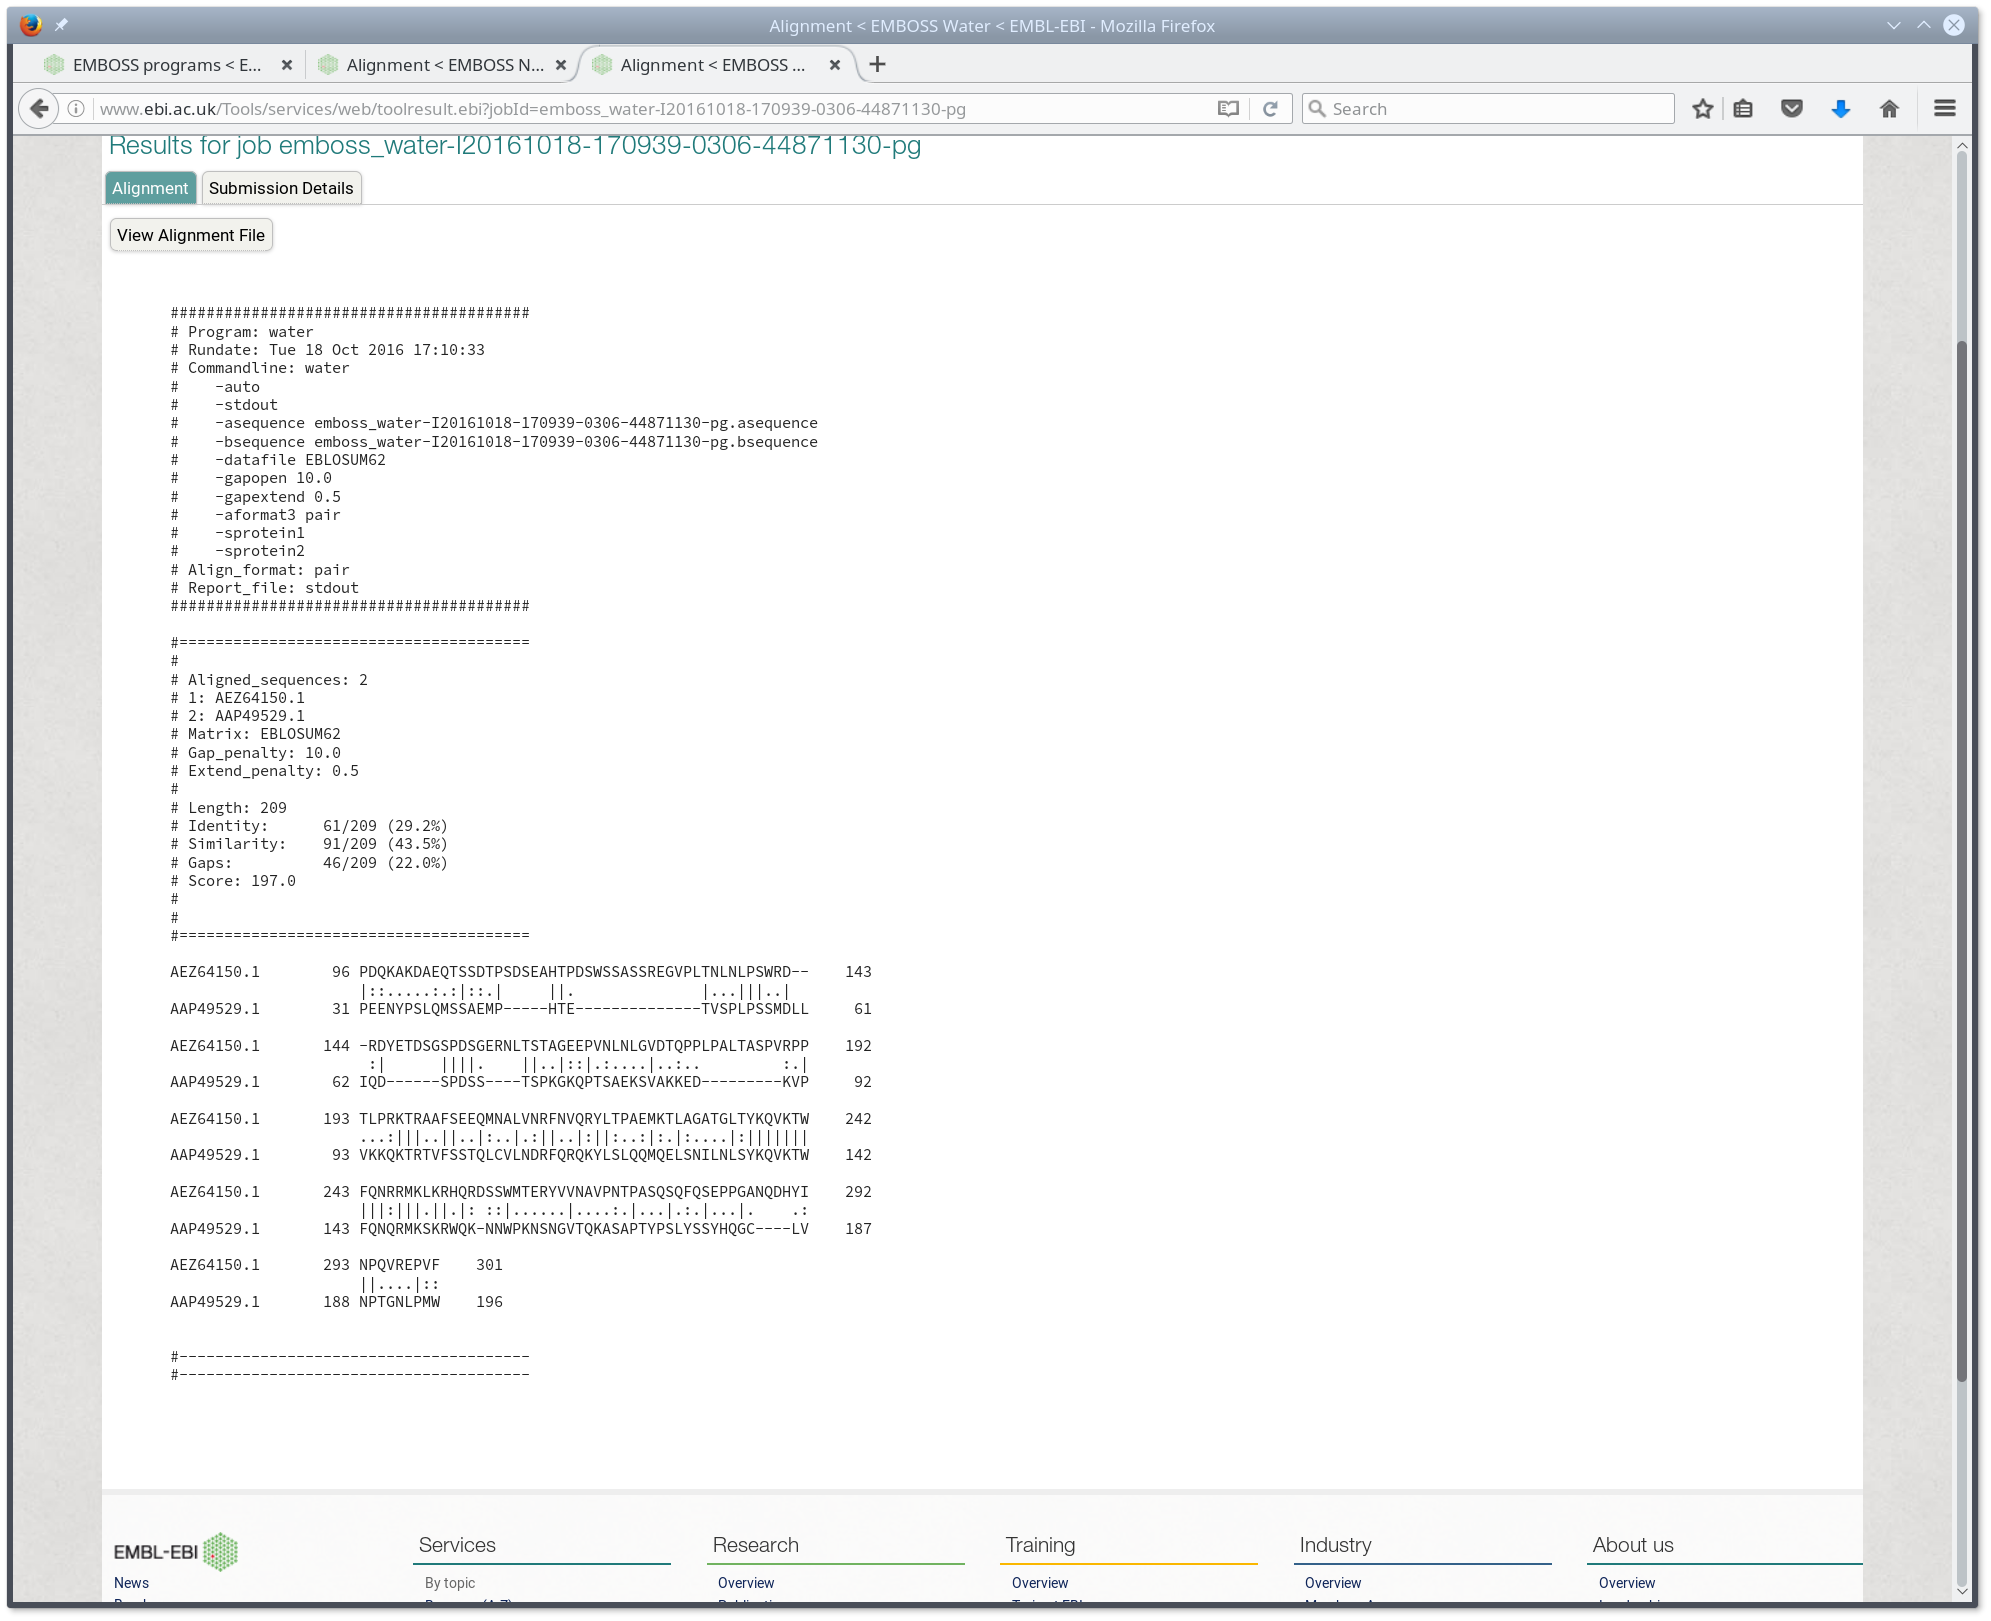
\includegraphics[width=0.9\textwidth]{images/emboss_water_result}
  \end{figure}
\end{frame}

\begin{frame}{Multiple alignment at EMBL}
  Clustal Omega: \url{http://www.ebi.ac.uk/Tools/msa/clustalo/}
  \begin{figure}[ht]
    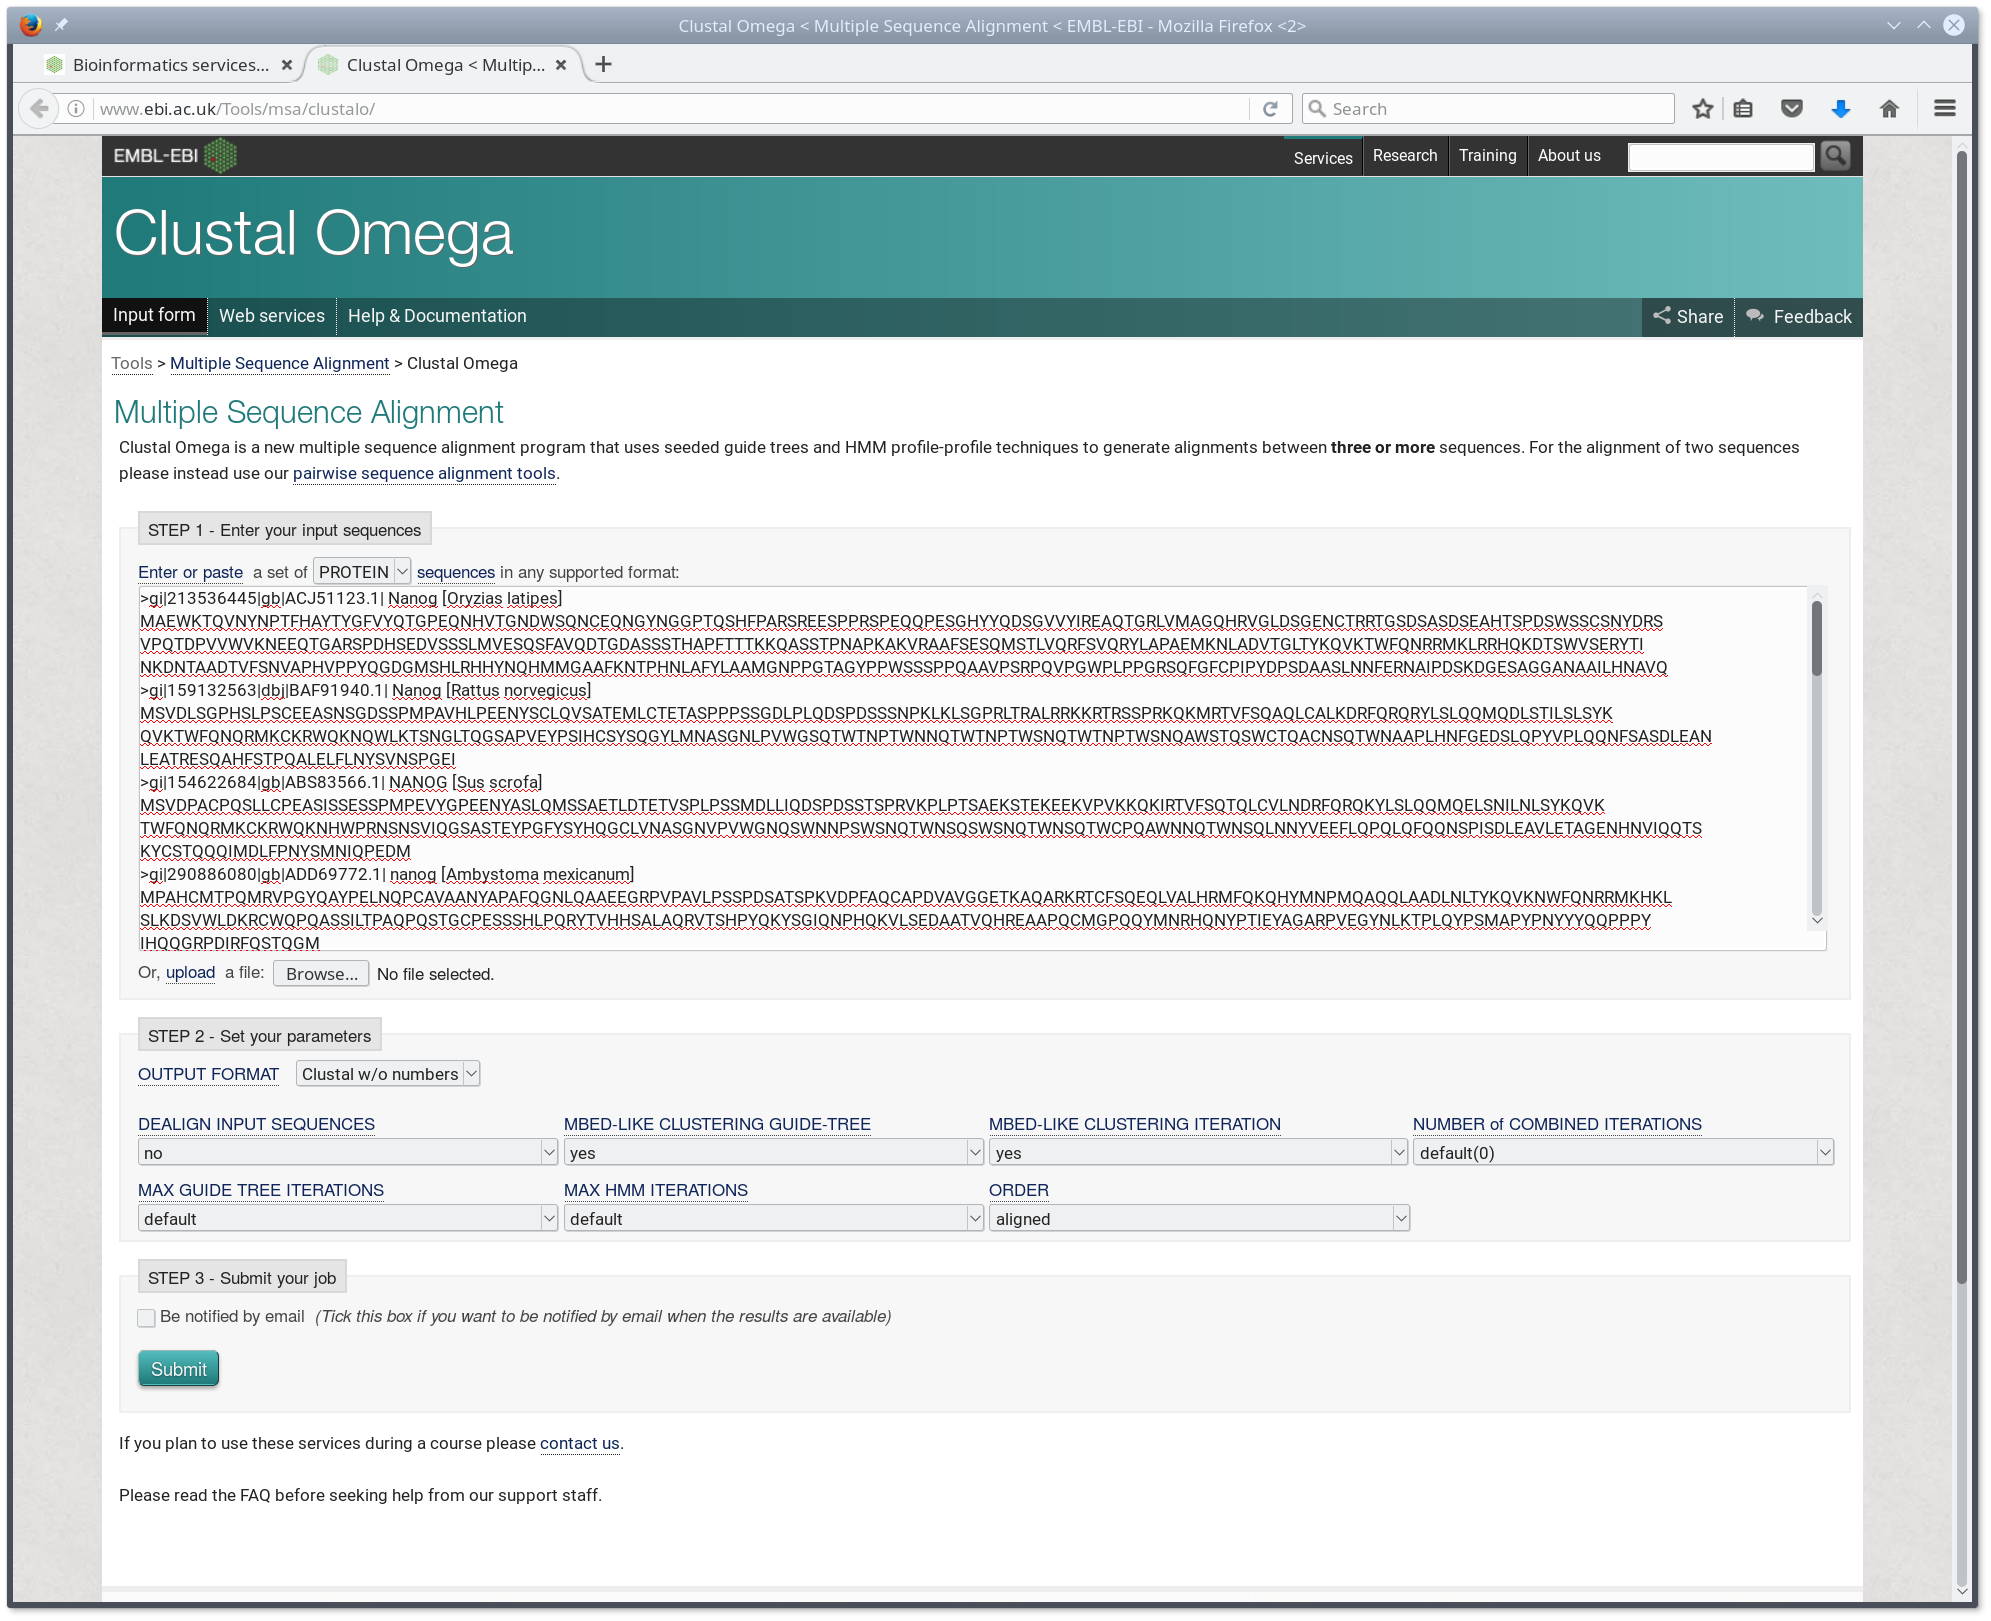
\includegraphics[width=0.8\textwidth]{images/ebi_clustalo}
  \end{figure}
\end{frame}

\begin{frame}{Multiple alignment at EMBL (2)}
  \begin{figure}[ht]
    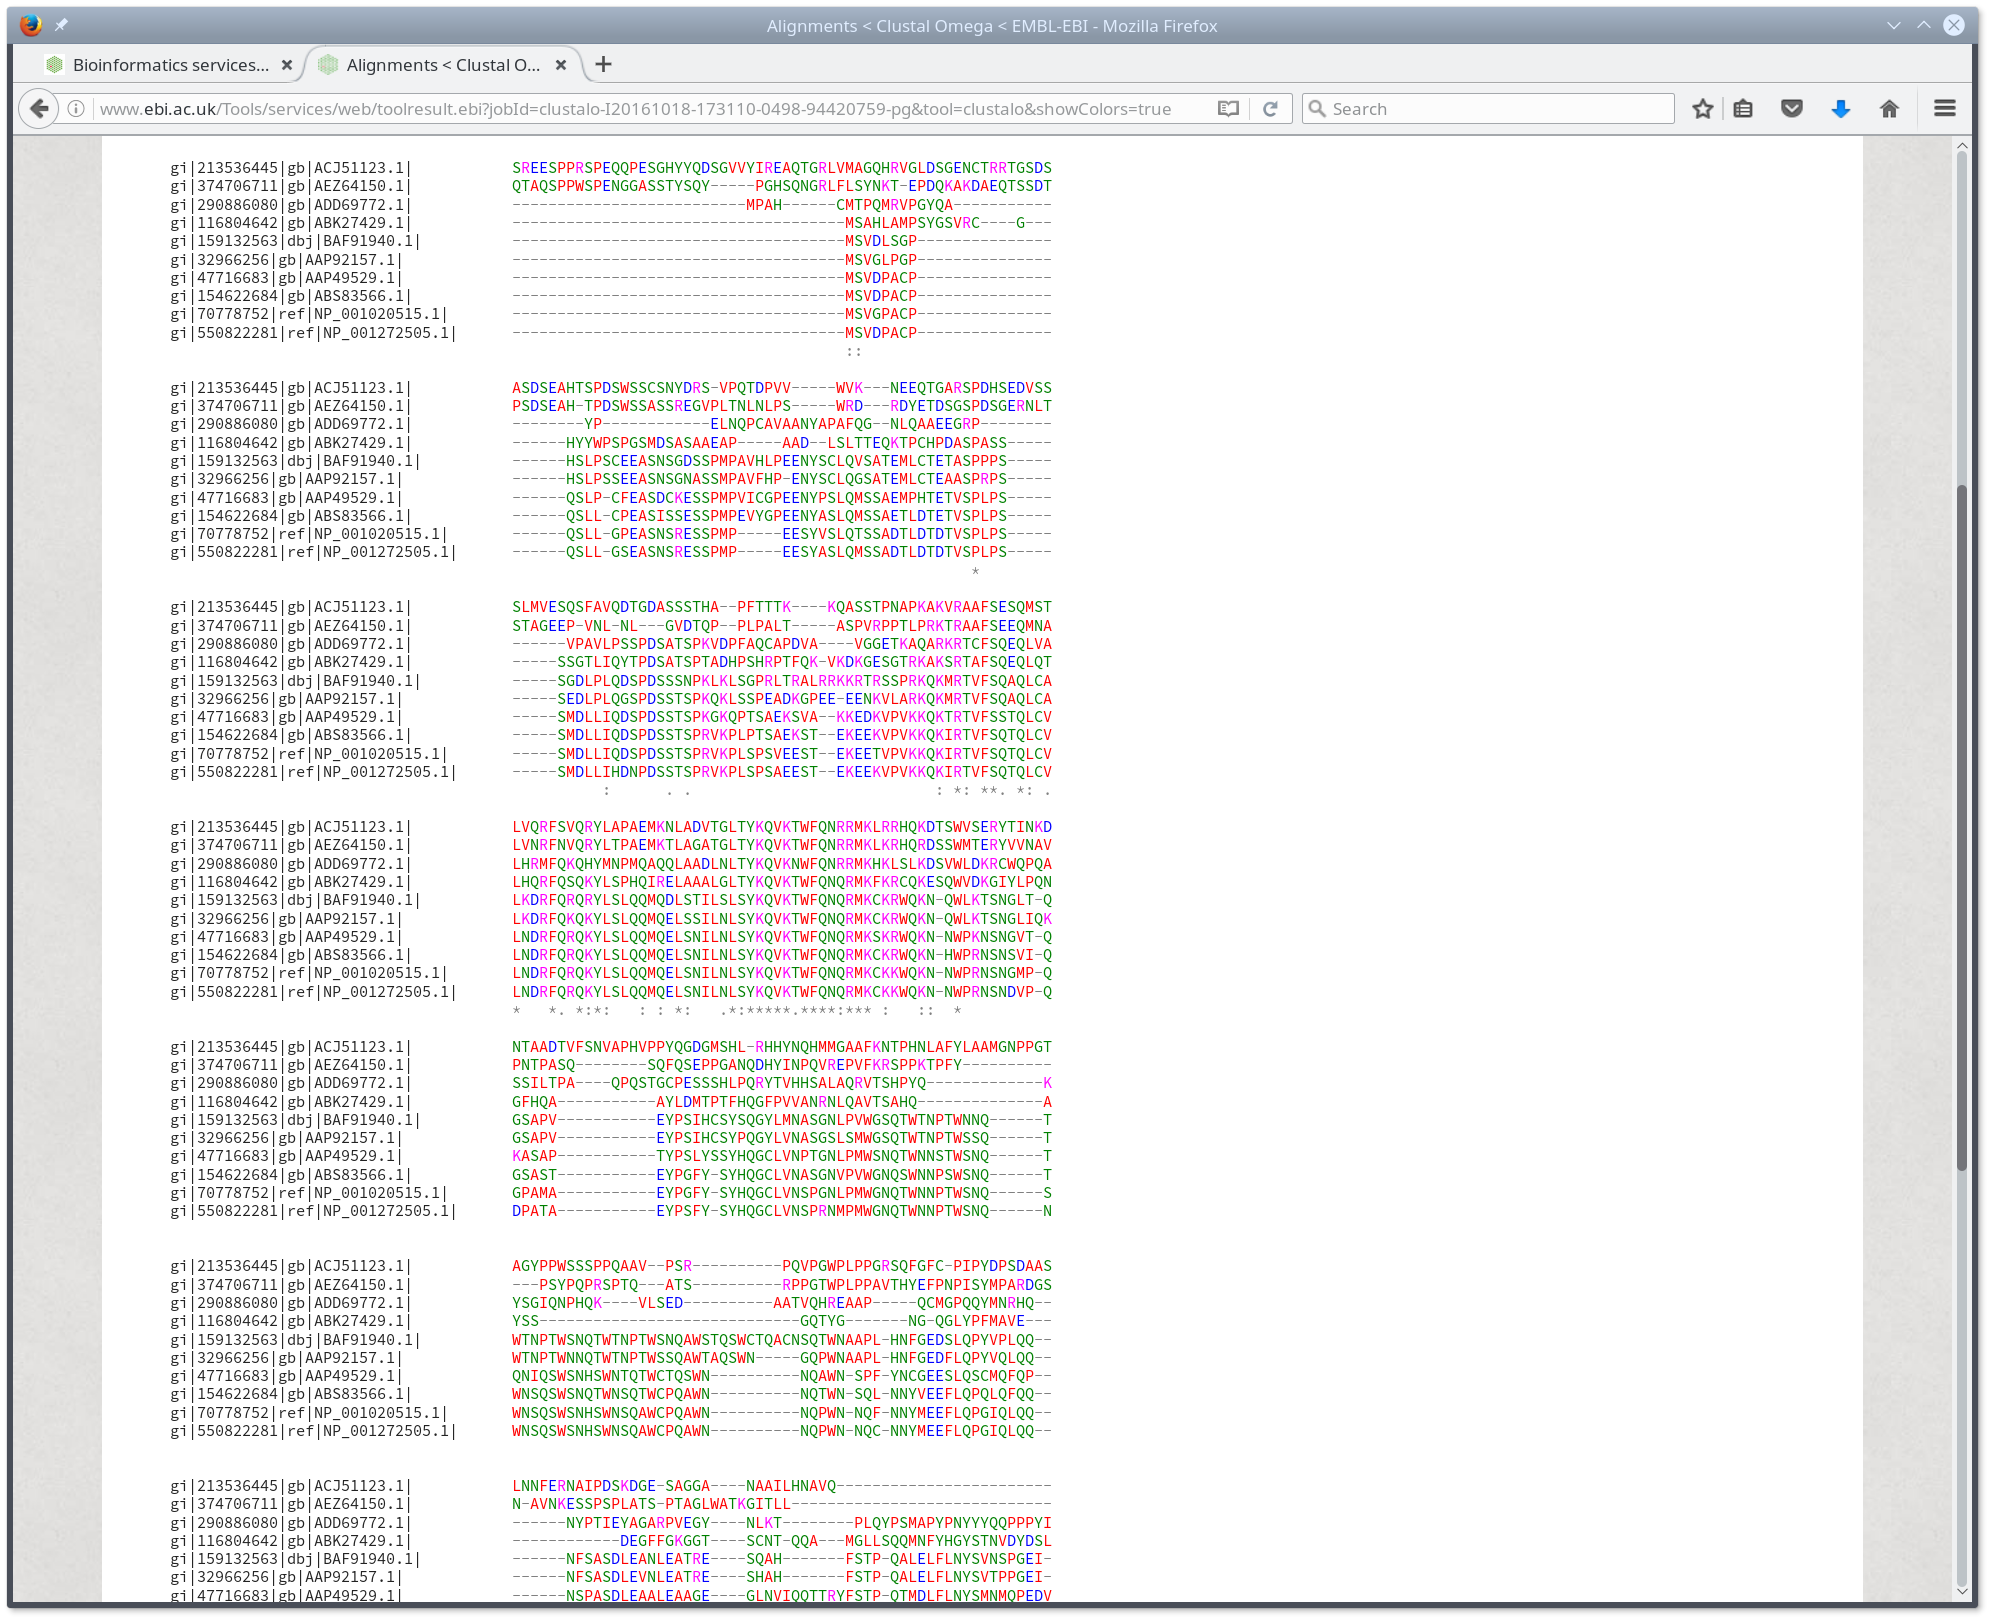
\includegraphics[width=0.9\textwidth]{images/ebi_clustalo_result}
  \end{figure}
\end{frame}

\begin{frame}{ClustalO to tree (1)}
  Note the \texttt{Phylogenetic Tree} obtained through:\\
  \texttt{Send to ClustalW2\_Phylogeny}
  \begin{figure}[ht]
    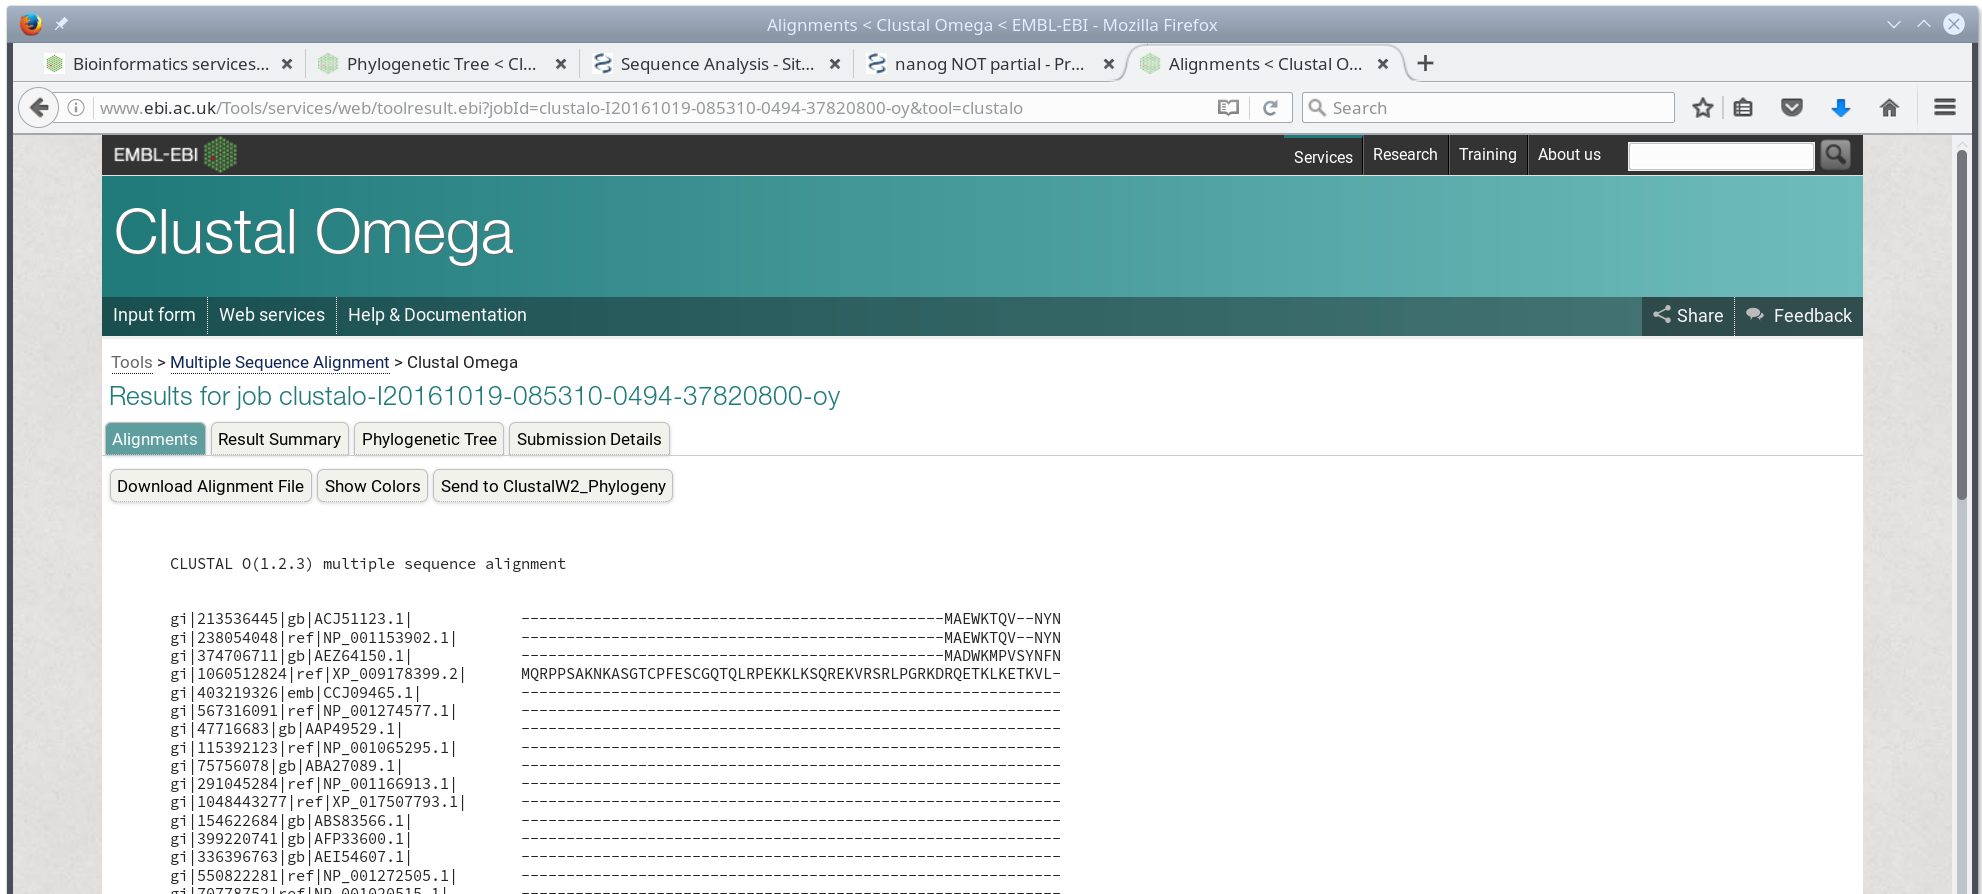
\includegraphics[width=0.9\textwidth]{images/ebi_clustalo_result_3.png}
  \end{figure}
\end{frame}

\begin{frame}{ClustalO to tree}
  \begin{figure}[ht]
    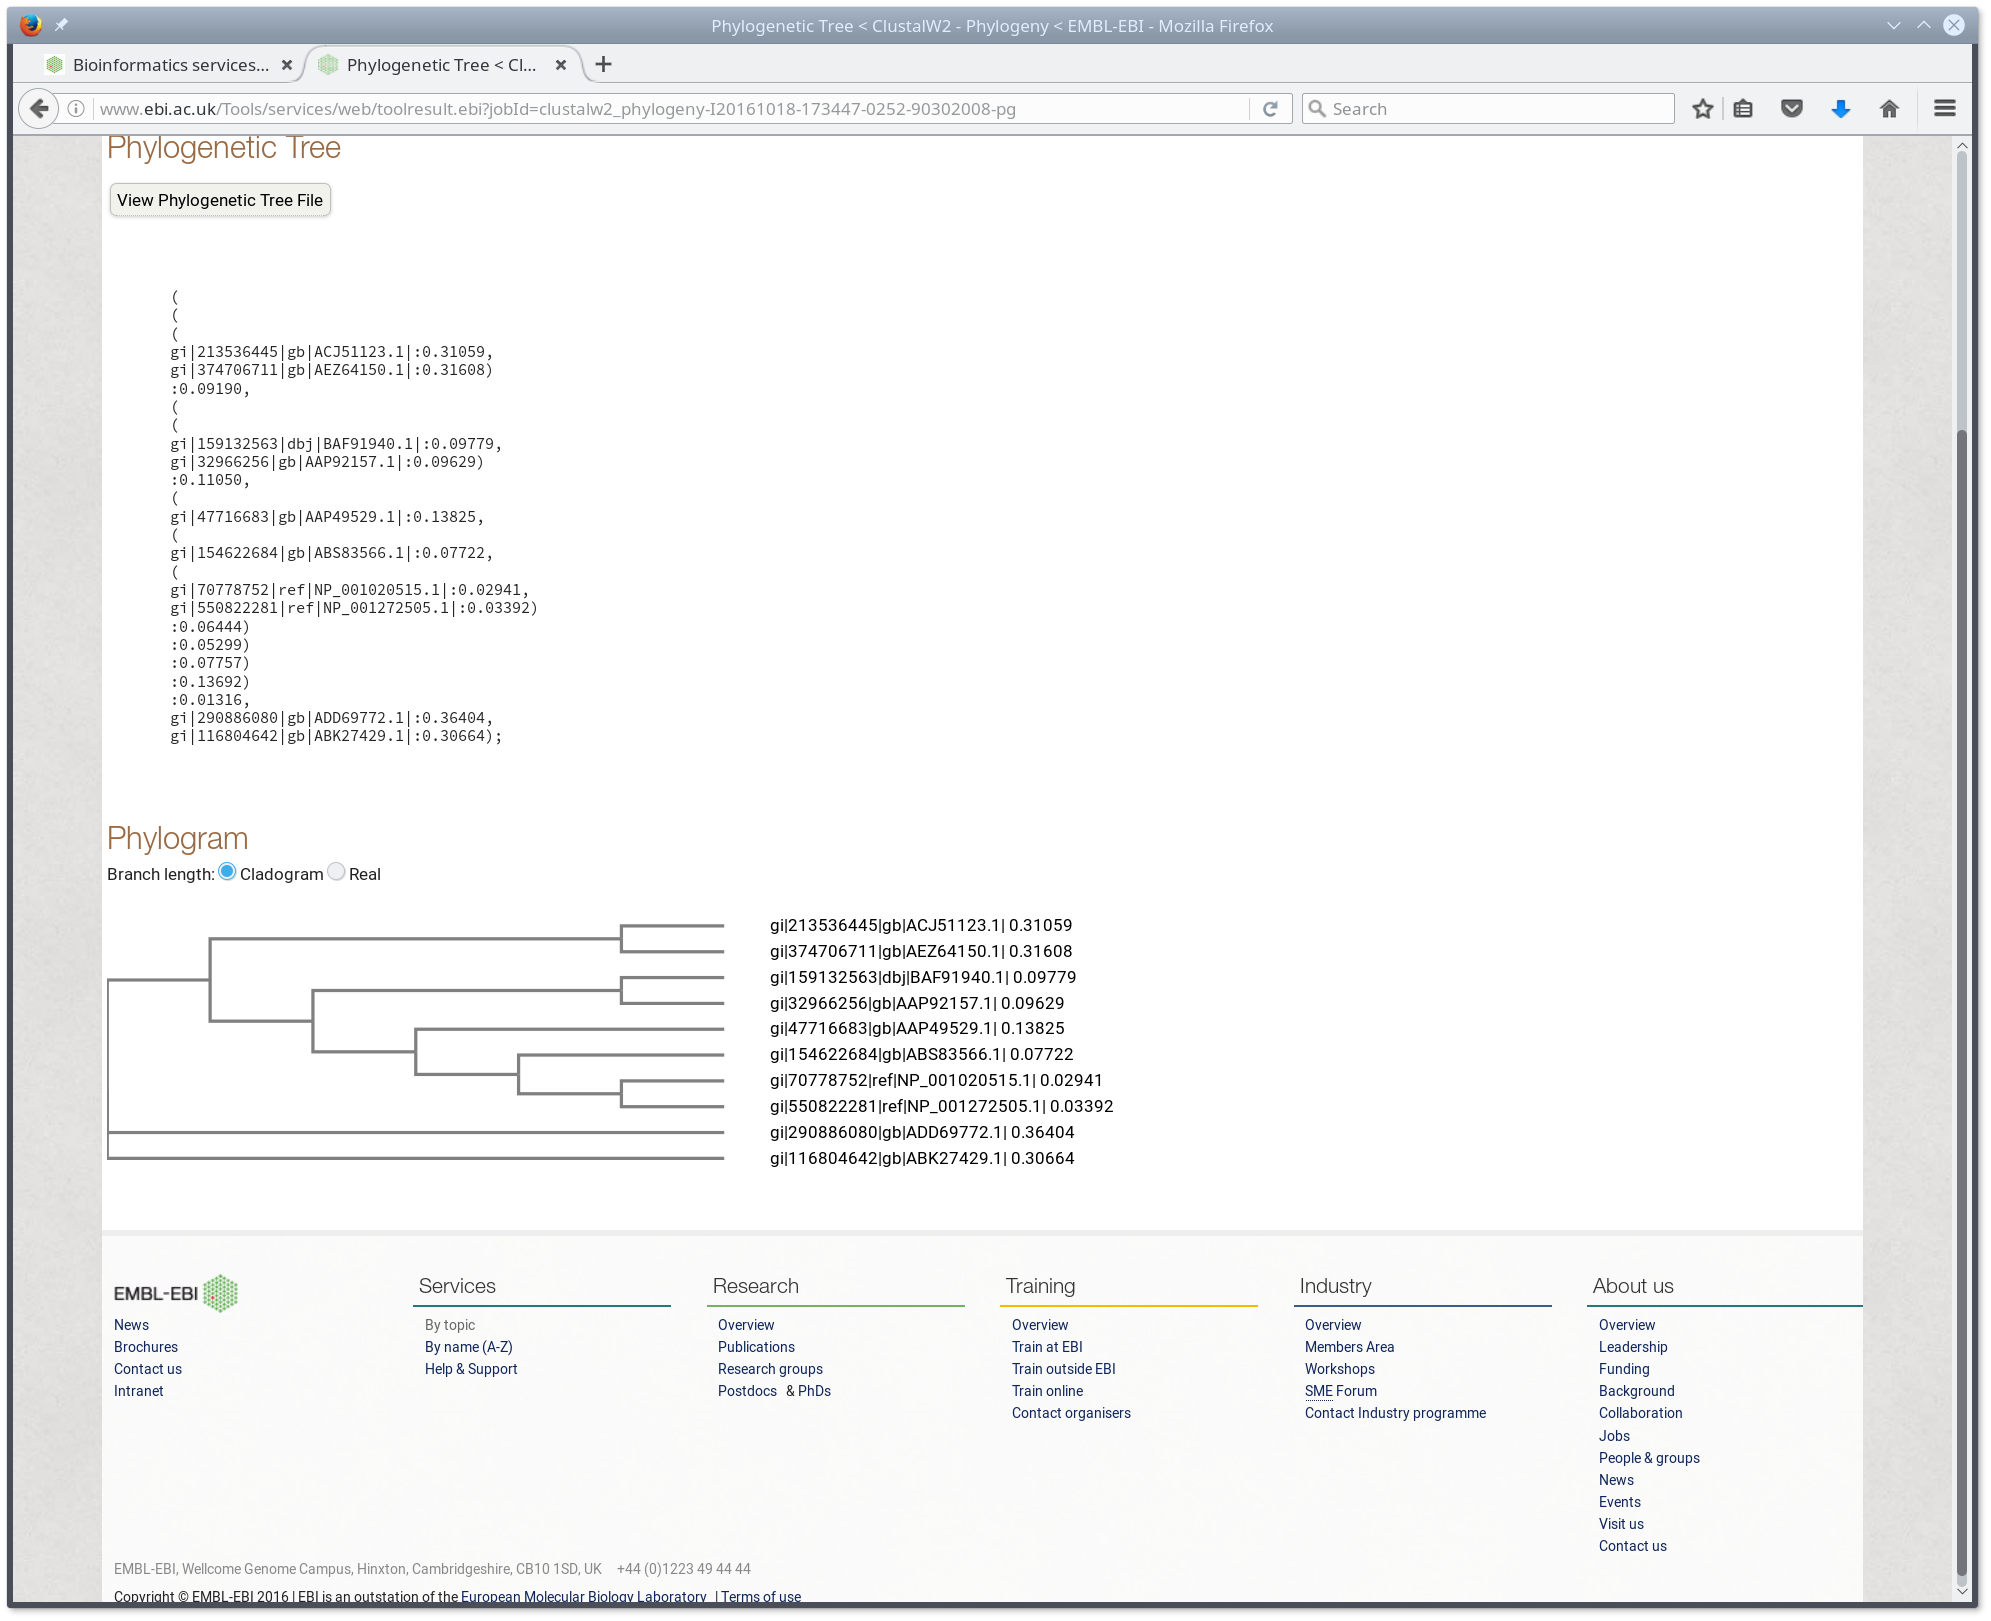
\includegraphics[width=0.95\textwidth]{images/ebi_clustalo_tree}
  \end{figure}
\end{frame}

\begin{frame}[fragile]{Sequence names / identifiers}
  Both the alignments and trees are difficult to look at, because we use
  sequence identifers from NCBI, like \verb#gi|19812342184|# that are not
  meaningful to humans;

  Nice to convert these to something useful. Again a small perl script is
  useful; can make the id something like \verb|genus_species_n| where
  \texttt{n} is used to seperate several sequences from the same species.
  
  How, depends on what set of sequences are used. Regardless you must always
  keep a map of the human readable to unique identifiers. Again, not easy
  without some automation.
\end{frame}

\begin{frame}{Converting sequence formats}
  EMBOSS Seqret \url{http://www.ebi.ac.uk/Tools/sfc/emboss_seqret/}
  \begin{figure}[ht]
    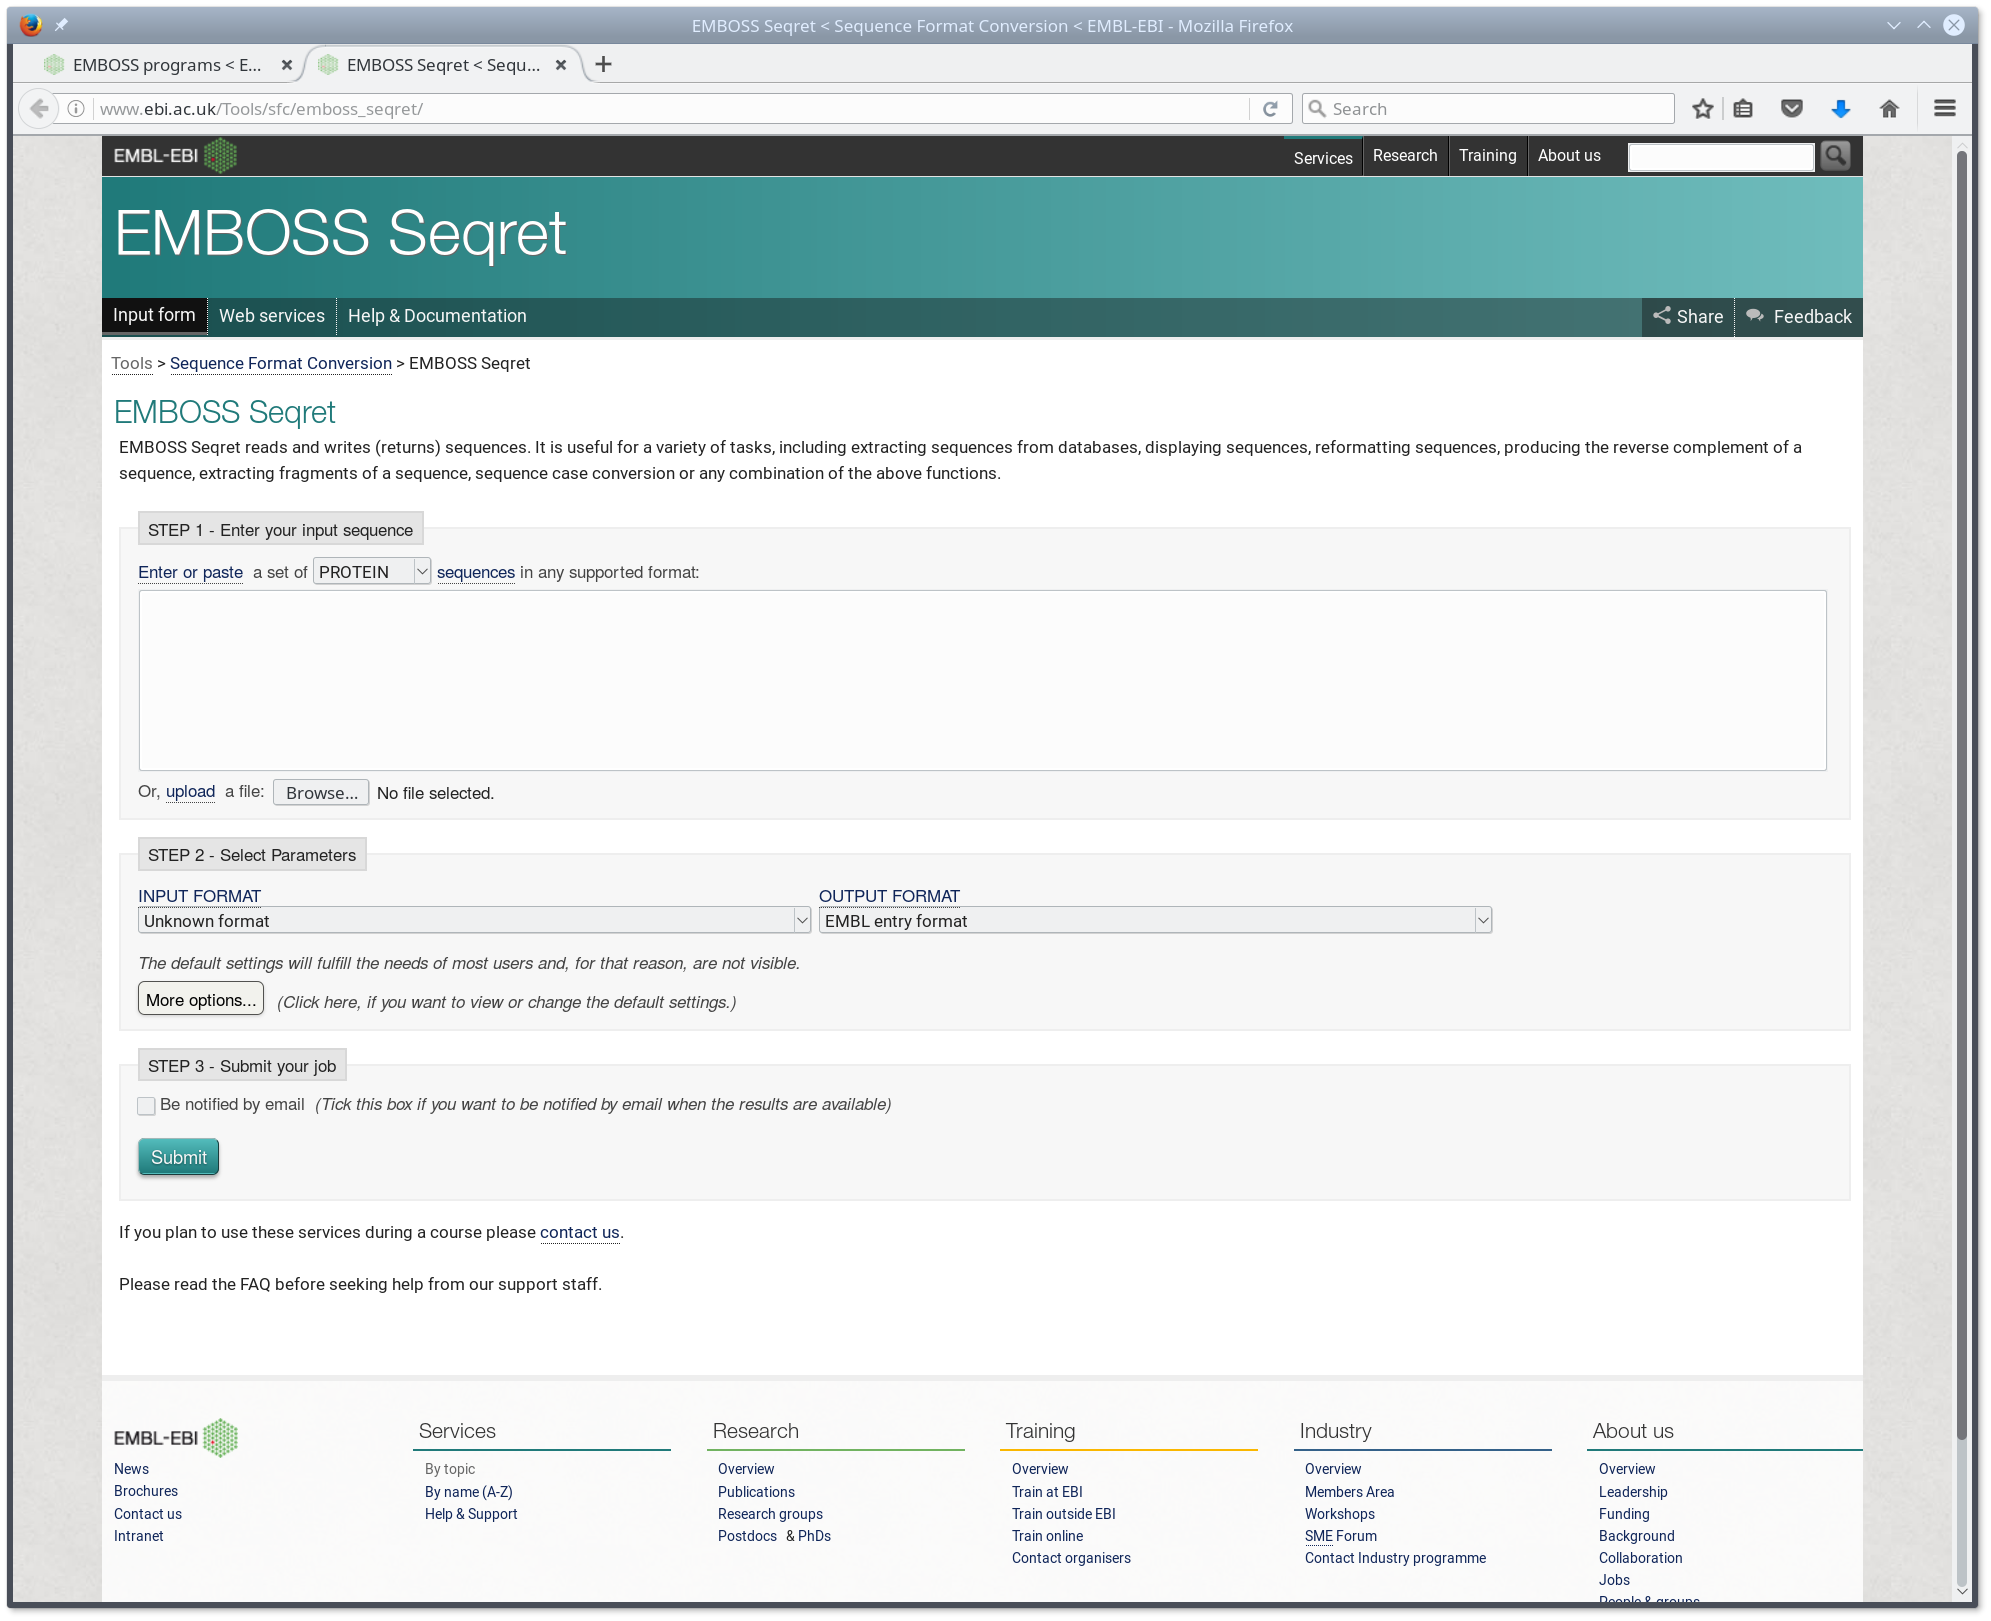
\includegraphics[width=0.8\textwidth]{images/emboss_seqret}
  \end{figure}
\end{frame}

\begin{frame}{Other EMBOSS tools}
  \begin{figure}[ht]
    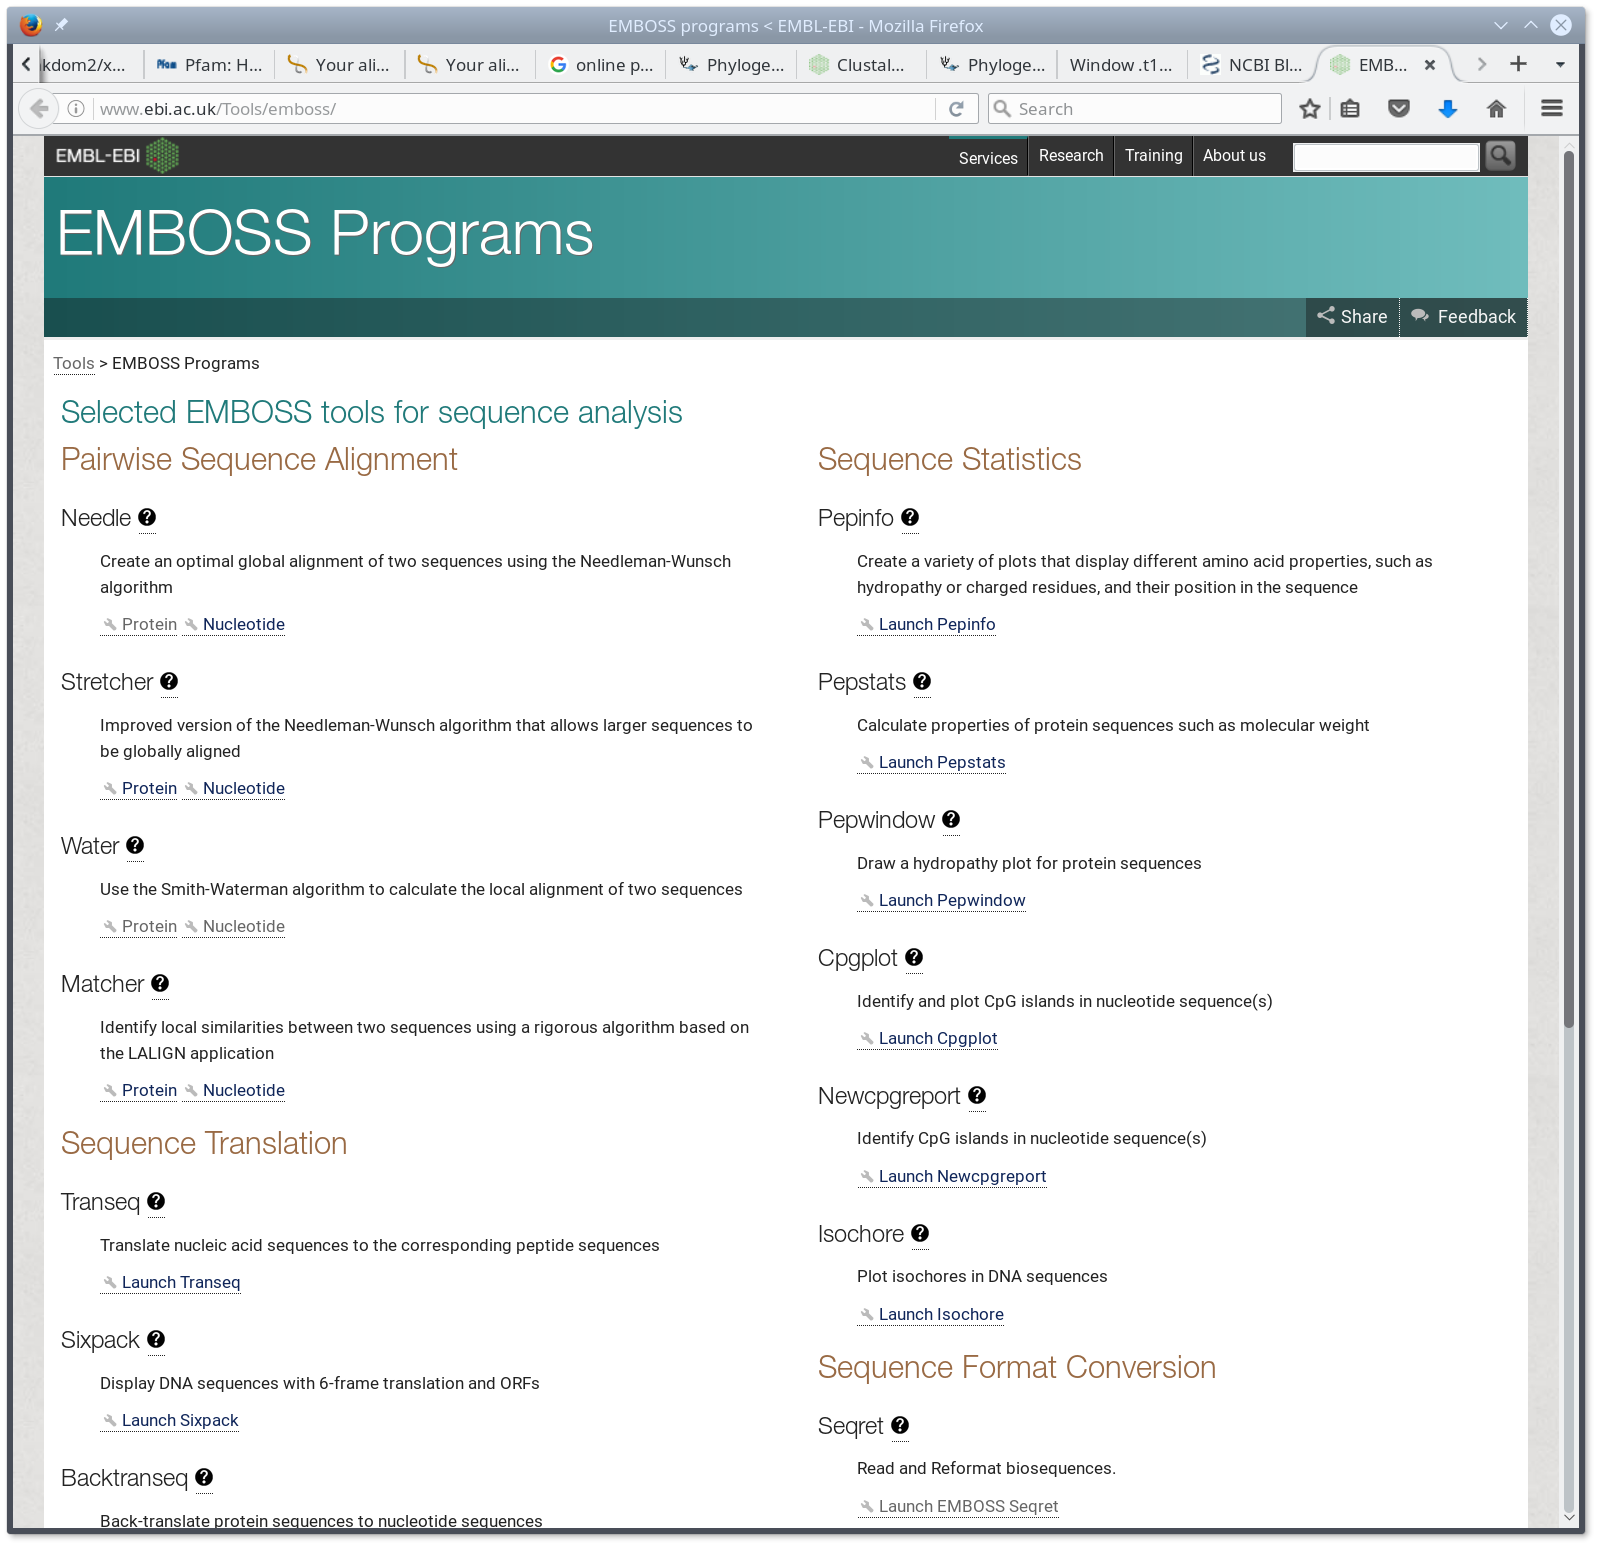
\includegraphics[width=0.8\textwidth]{images/emboss_tools}
  \end{figure}

\end{frame}

\begin{frame}{Interesting NCBI tools}
  \begin{itemize}
    \item BLAST Link (BLink): pre-computed blast for all proteins\\
      \url{https://www.ncbi.nlm.nih.gov/sutils/blink.cgi?mode=query}
    \item BLAST: various blast programs\\
      \url{https://blast.ncbi.nlm.nih.gov/}
    \item ORF Finder: finds open reading frames\\
      \url{https://www.ncbi.nlm.nih.gov/orffinder/}
    \item Sequence Viewer\\
      \url{https://www.ncbi.nlm.nih.gov/guide/sequence-analysis/}
    \item VecScreen: identifies vector sequences
      \url{https://www.ncbi.nlm.nih.gov/projects/sviewer/}  
  \end{itemize}
\end{frame}

\begin{frame}{pre-computed blast}
  BLINK
  \begin{figure}[ht]
    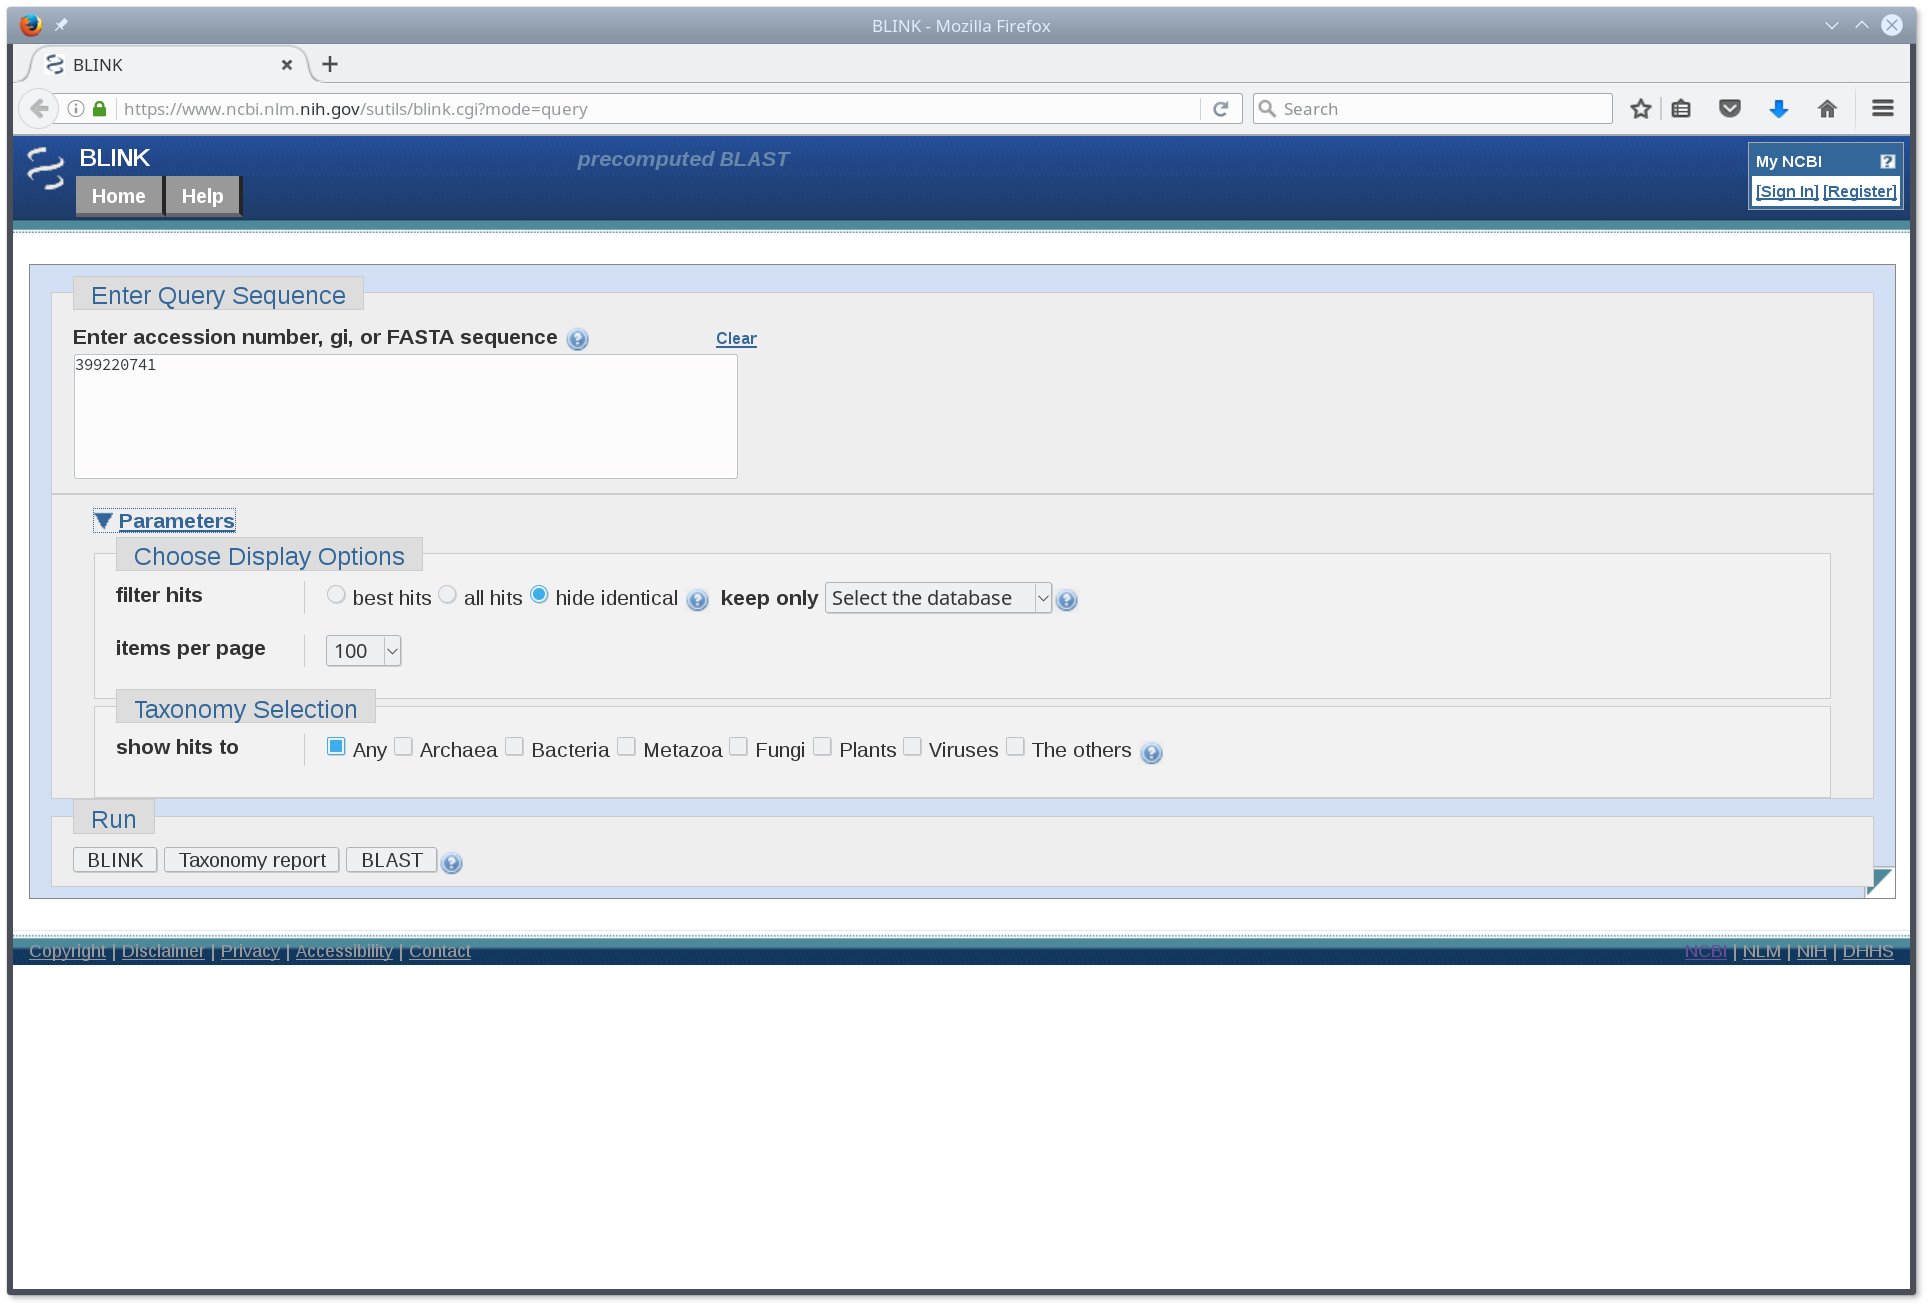
\includegraphics[width=0.8\textwidth]{images/ncbi_blink_1}
  \end{figure}
  
  \small need an identifer or sequence\\
  3 options: BLINK, Taxonomy report, BLAST
\end{frame}

\begin{frame}{BLINK results}
  \begin{figure}[ht]
    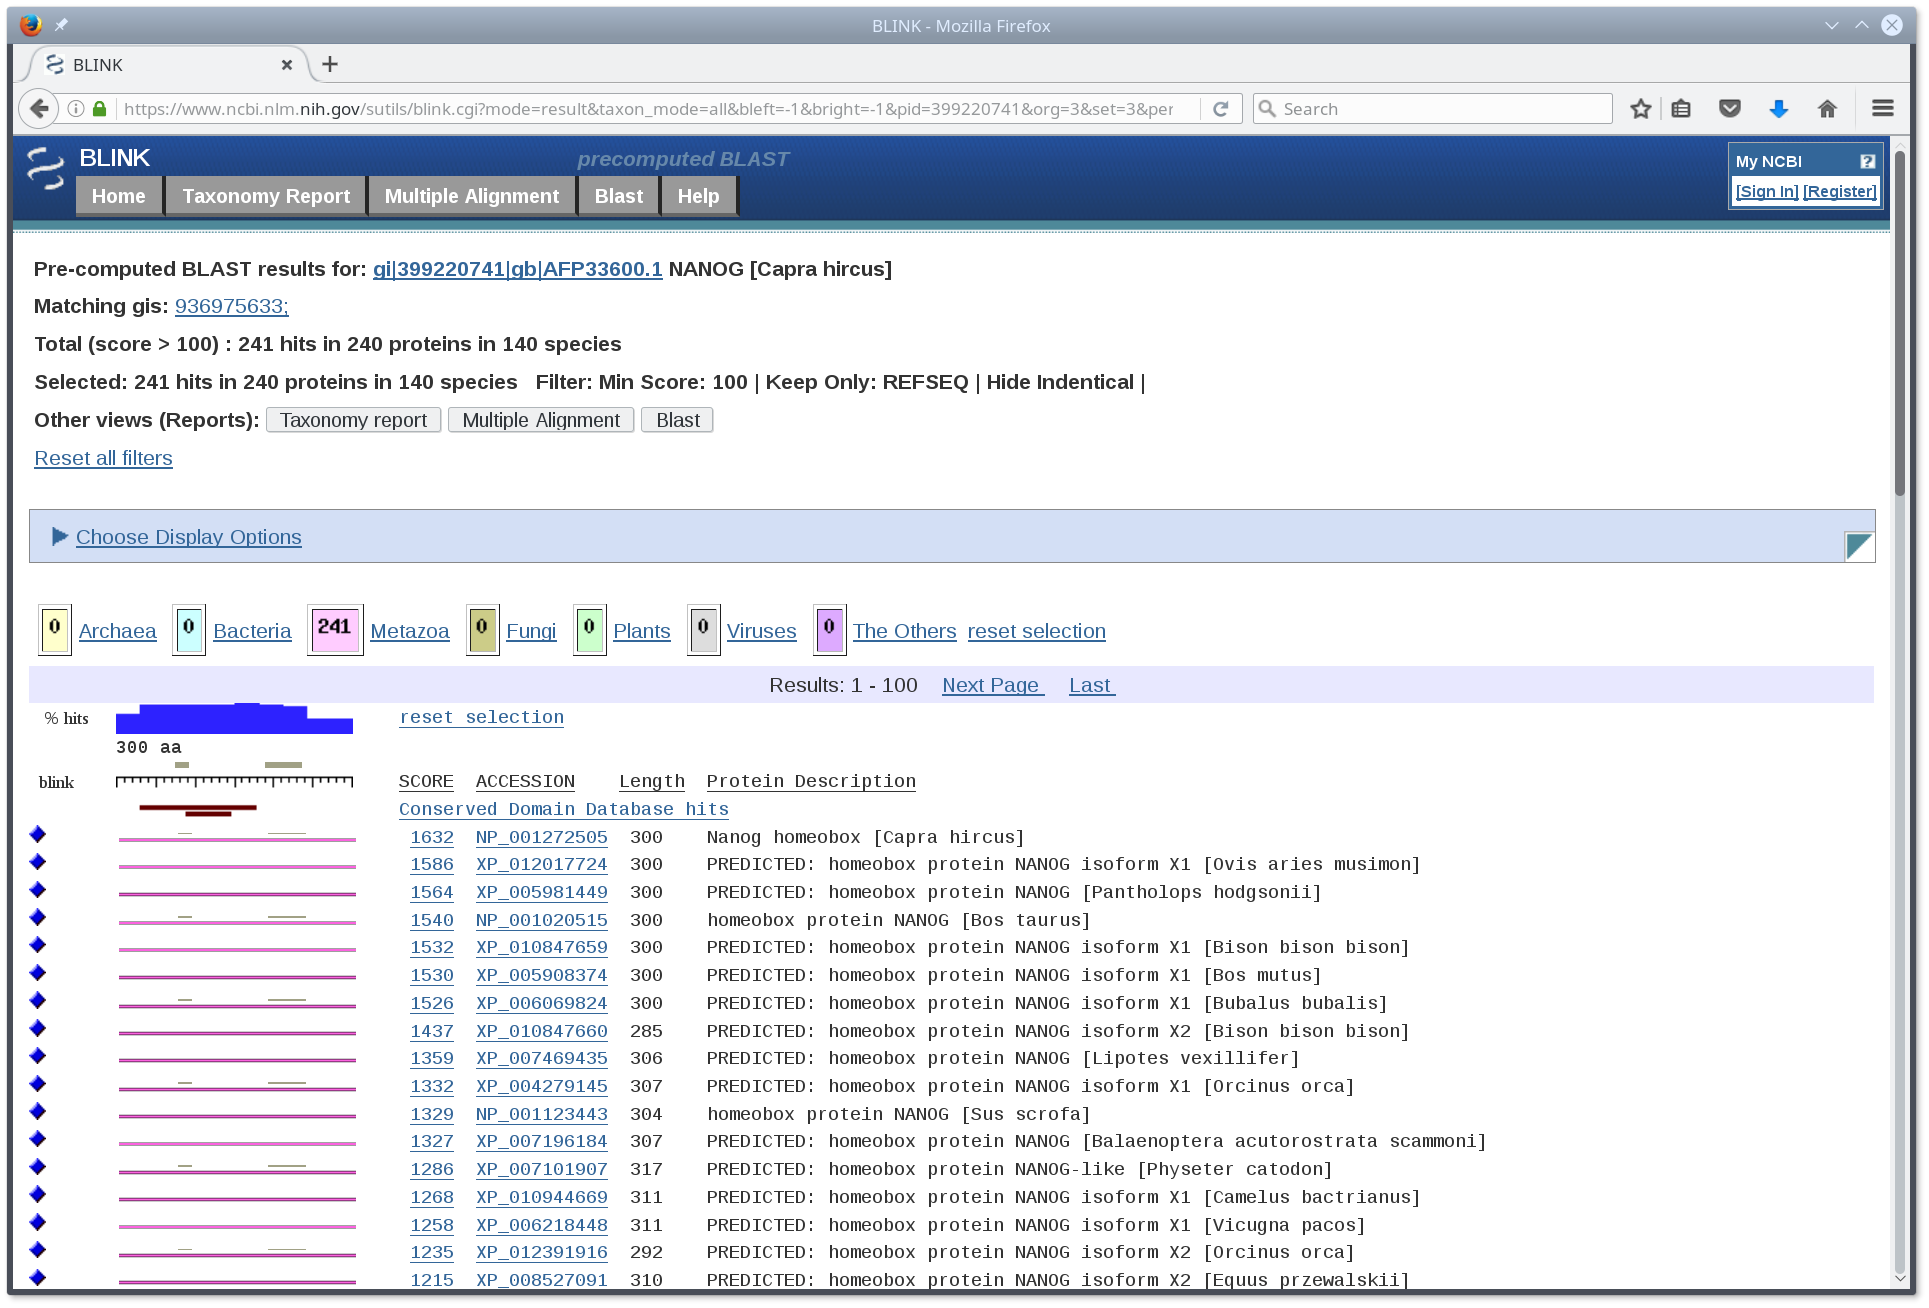
\includegraphics[width=0.9\textwidth]{images/ncbi_blink_2}
  \end{figure}
\end{frame}

\begin{frame}{BLINK: Conserved domains}
  PGC7/Stella/Dppa3 domain:
  \begin{figure}[ht]
    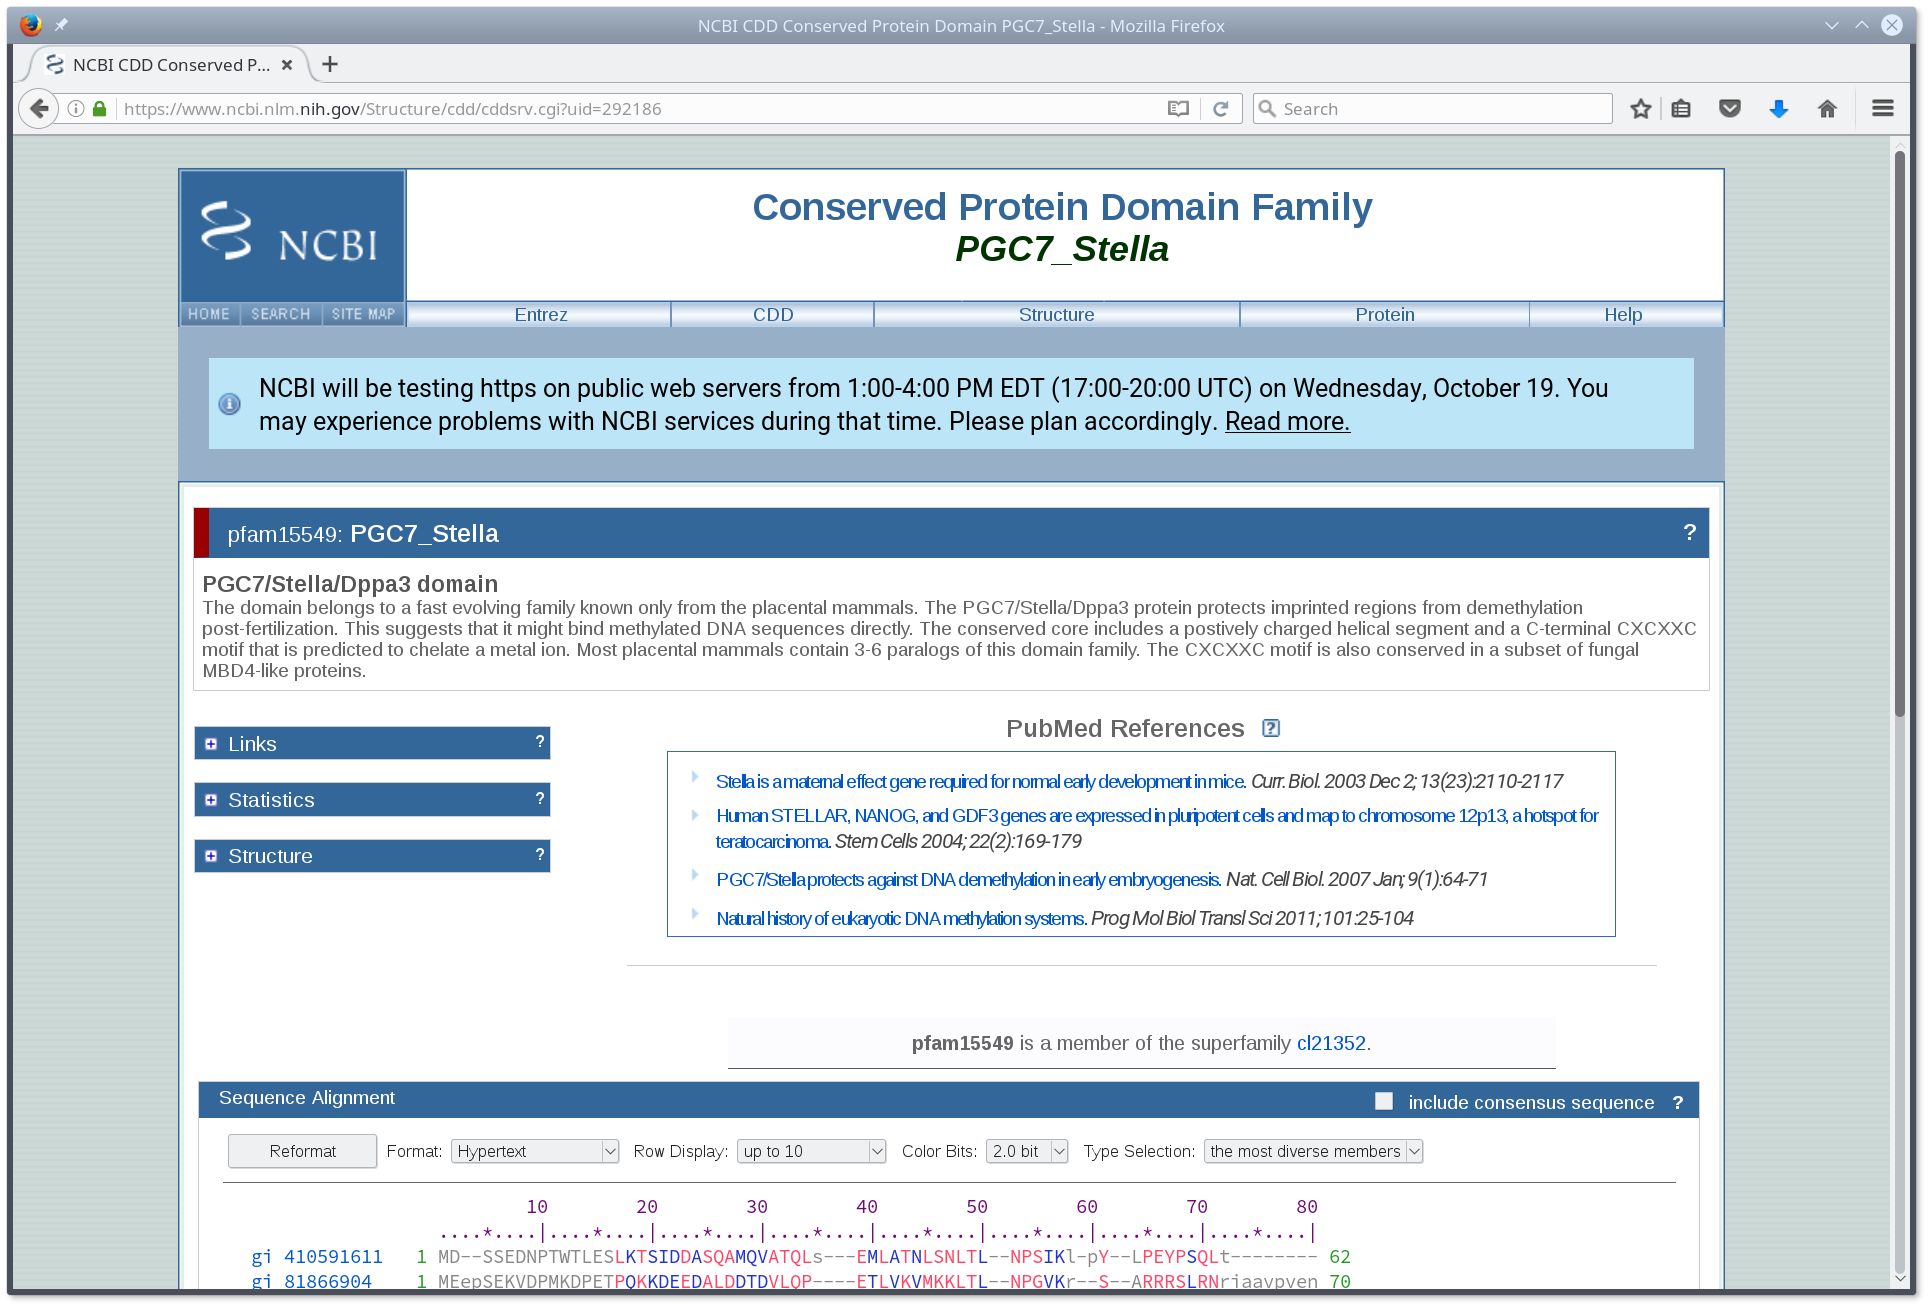
\includegraphics[width=0.9\textwidth]{images/ncbi_blink_3}
  \end{figure}
  
\end{frame}

\begin{frame}{BLINK: Multiple Sequence alignment}
  \begin{figure}[ht]
    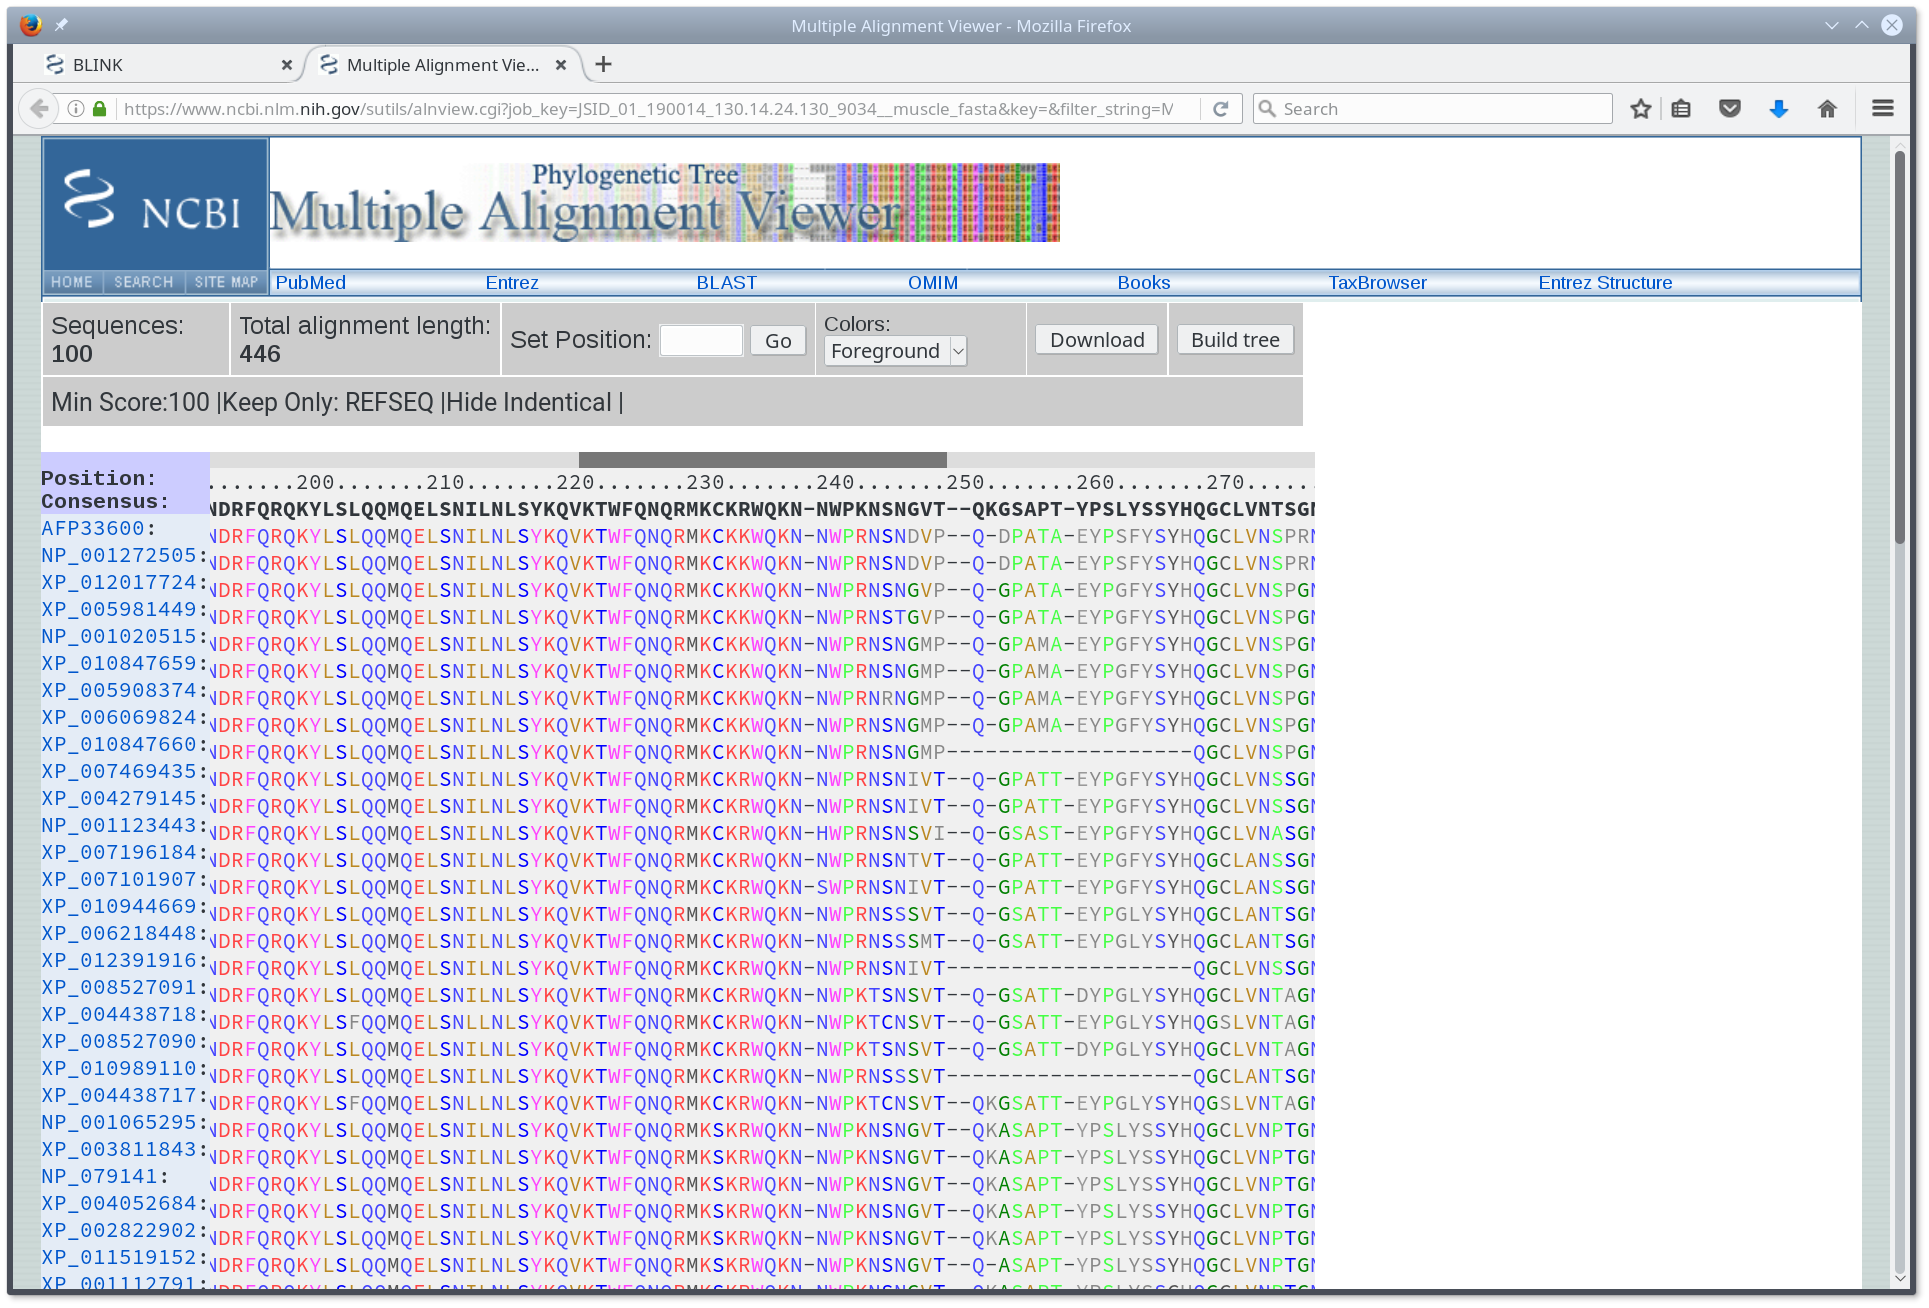
\includegraphics[width=0.9\textwidth]{images/ncbi_blink_4}
  \end{figure}
\end{frame}

\begin{frame}{BLINK: Taxonomy report}
  \begin{figure}[ht]
    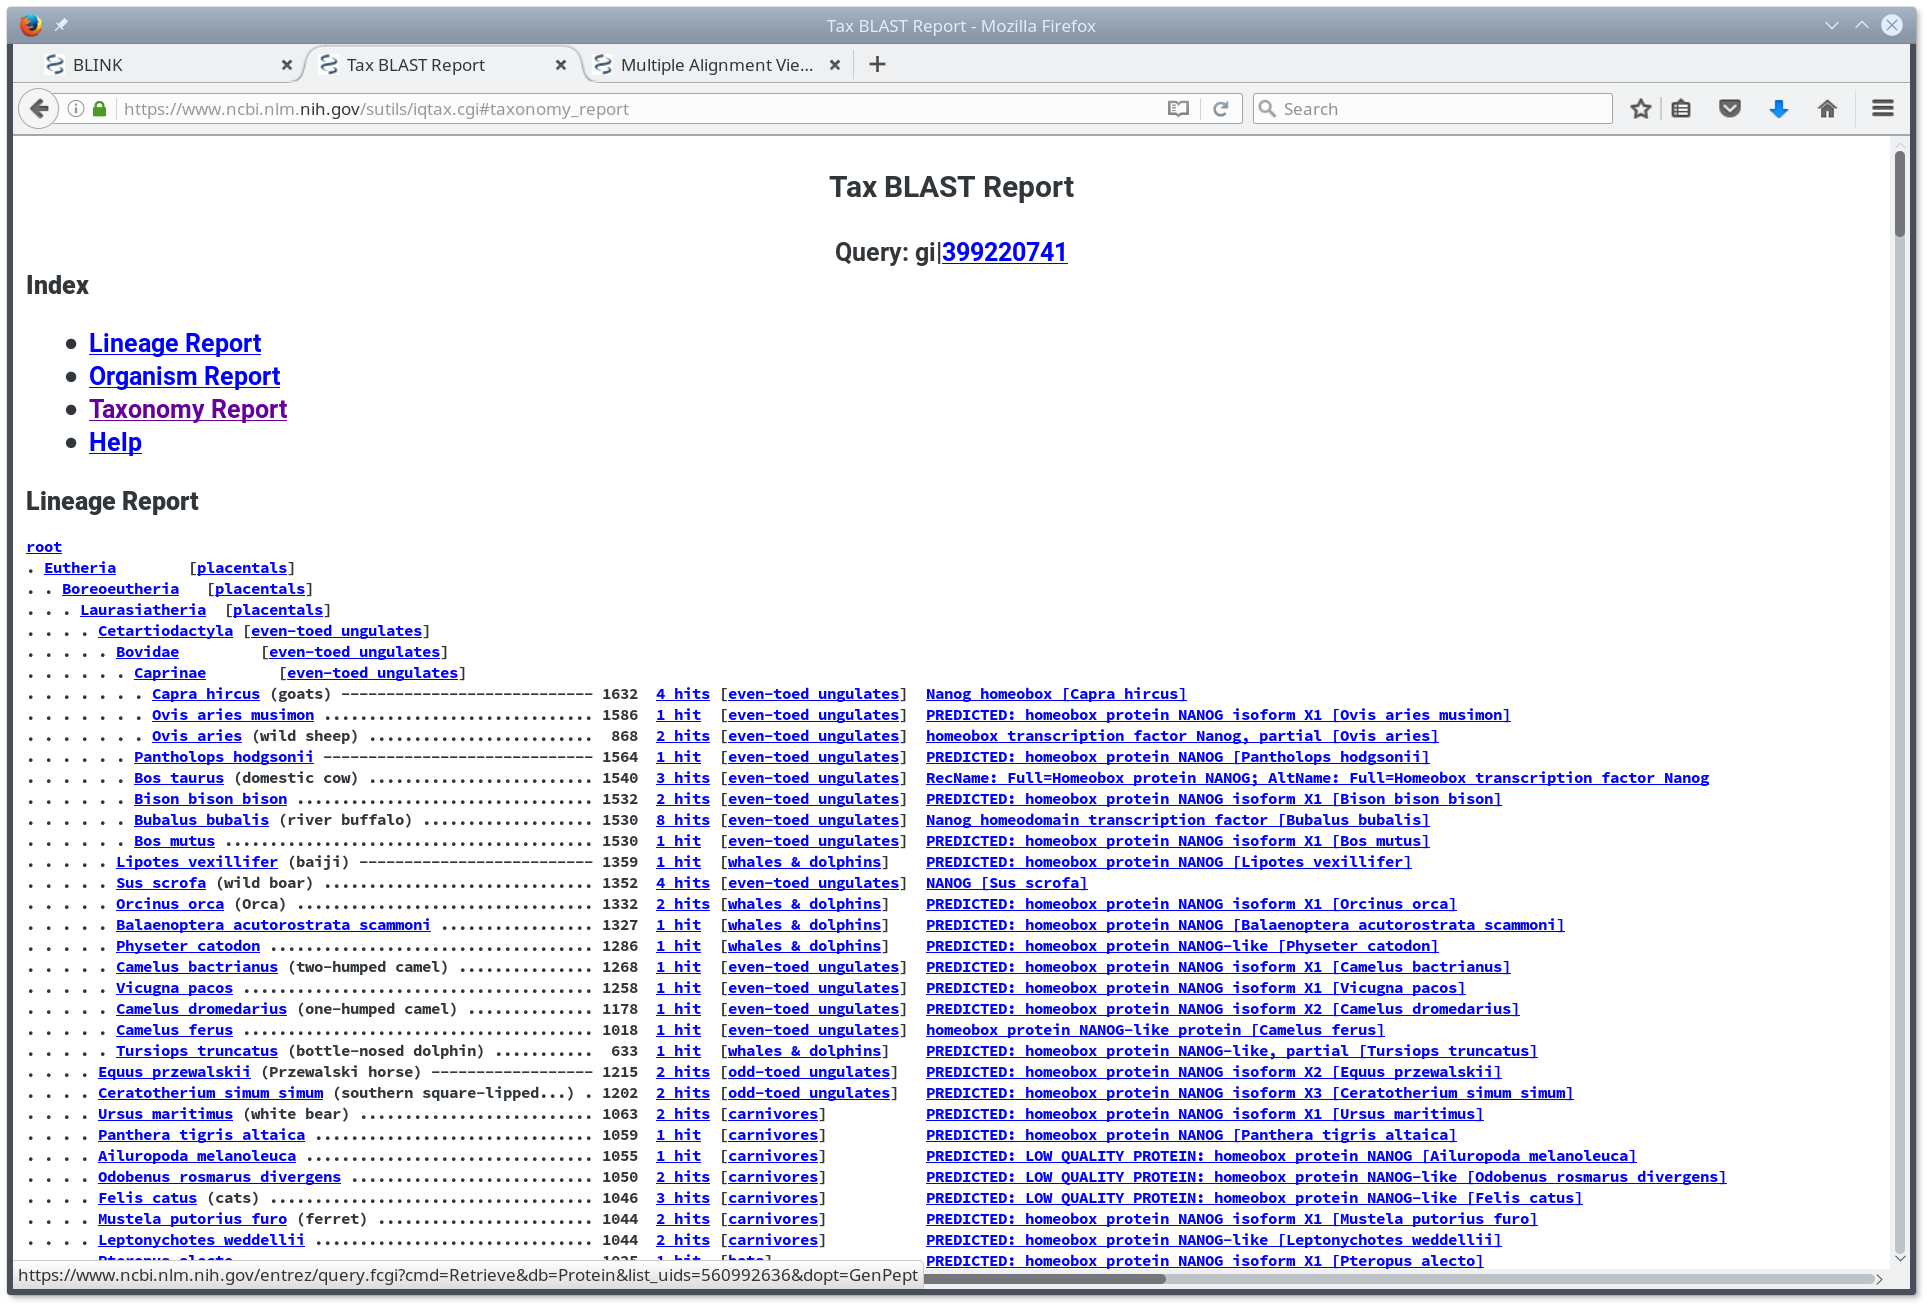
\includegraphics[width=0.9\textwidth]{images/ncbi_blink_5}
  \end{figure}
\end{frame}

\begin{frame}{BLINK: MSA outputs}
  \begin{figure}[ht]
    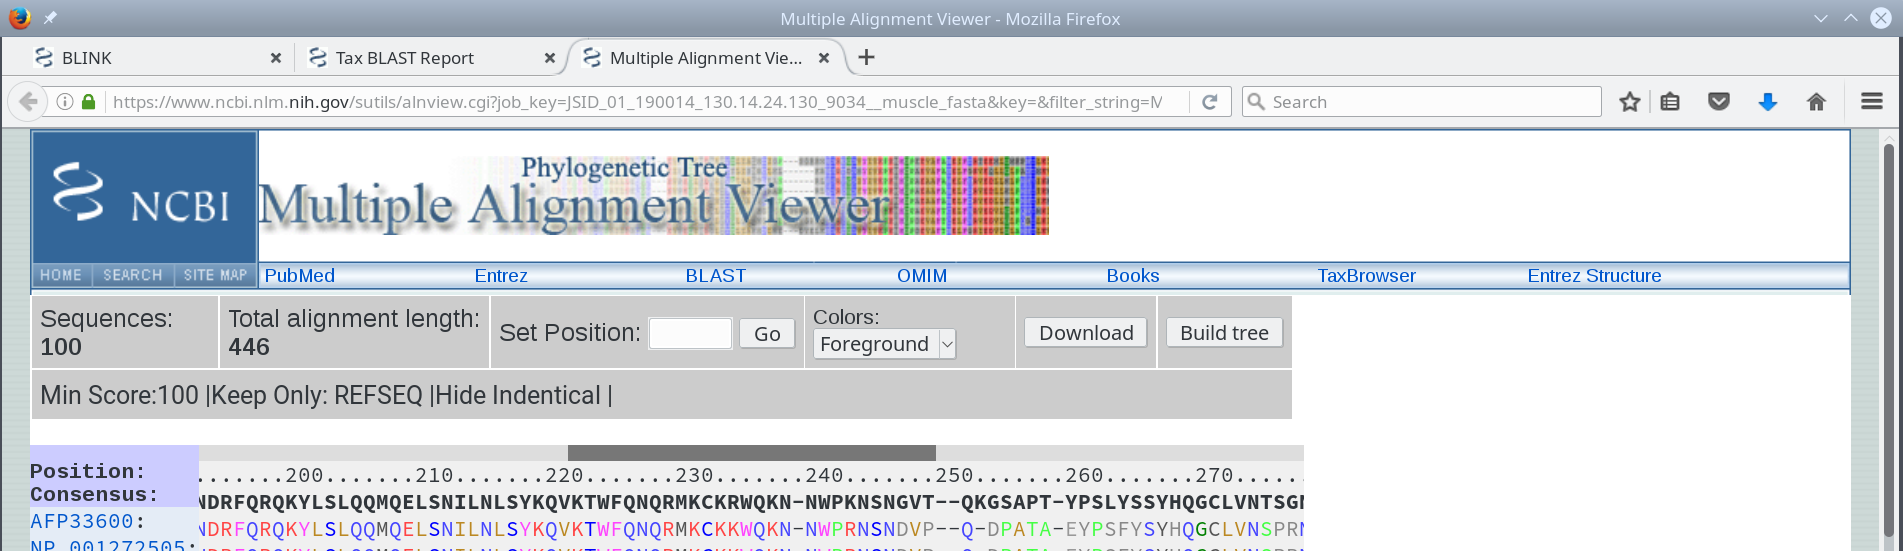
\includegraphics[width=0.9\textwidth]{images/ncbi_blink_6}
  \end{figure}

  \begin{itemize}
    \item Download alignment
    \item Build tree
  \end{itemize}
\end{frame}

\begin{frame}{BLINK: Tree}
  \begin{figure}[ht]
    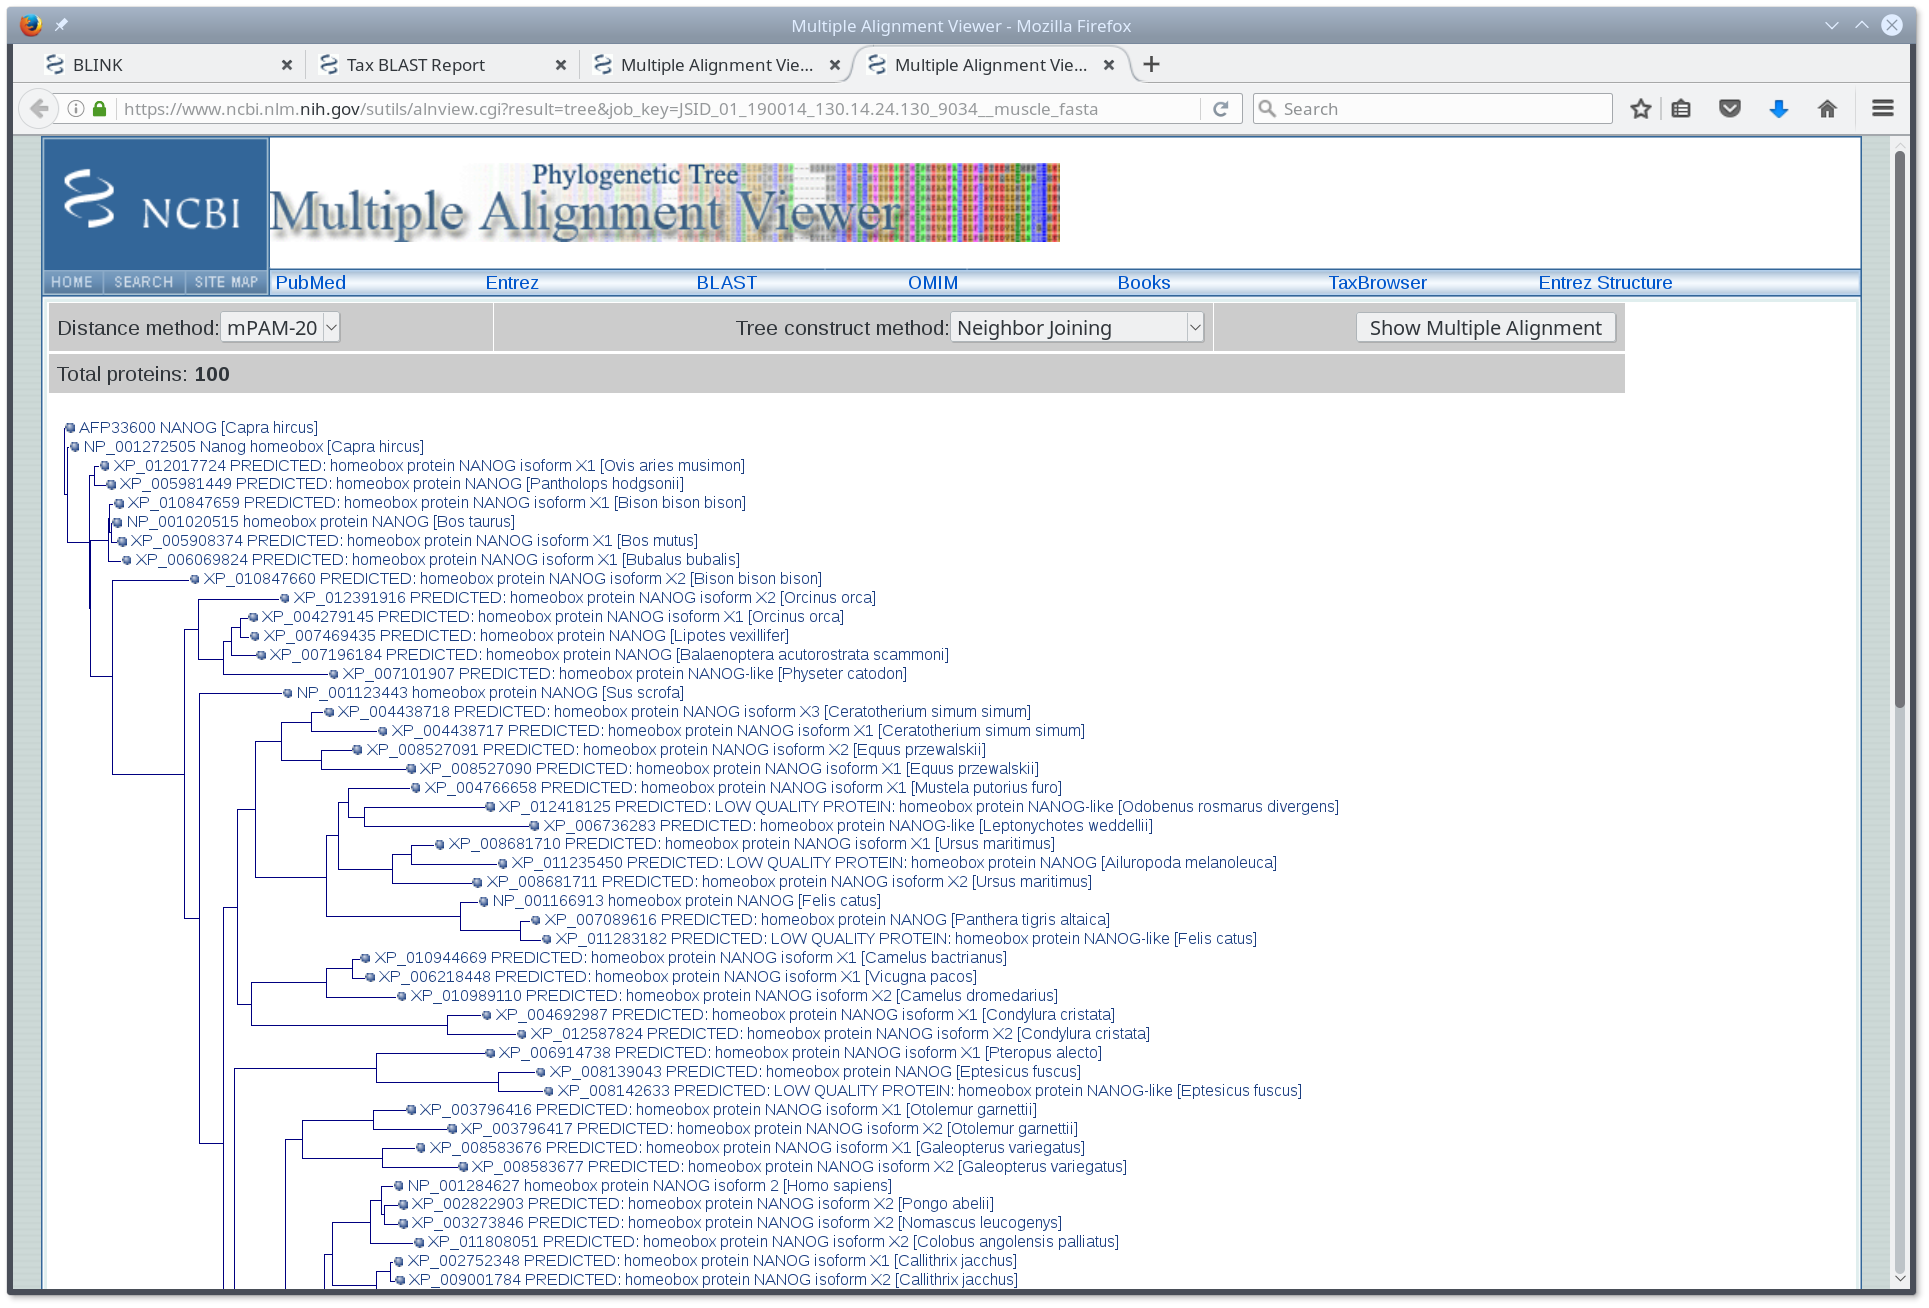
\includegraphics[width=0.9\textwidth]{images/ncbi_blink_7}
  \end{figure}
\end{frame}

\begin{frame}{Downloaded alignment?}
  \begin{figure}[ht]
    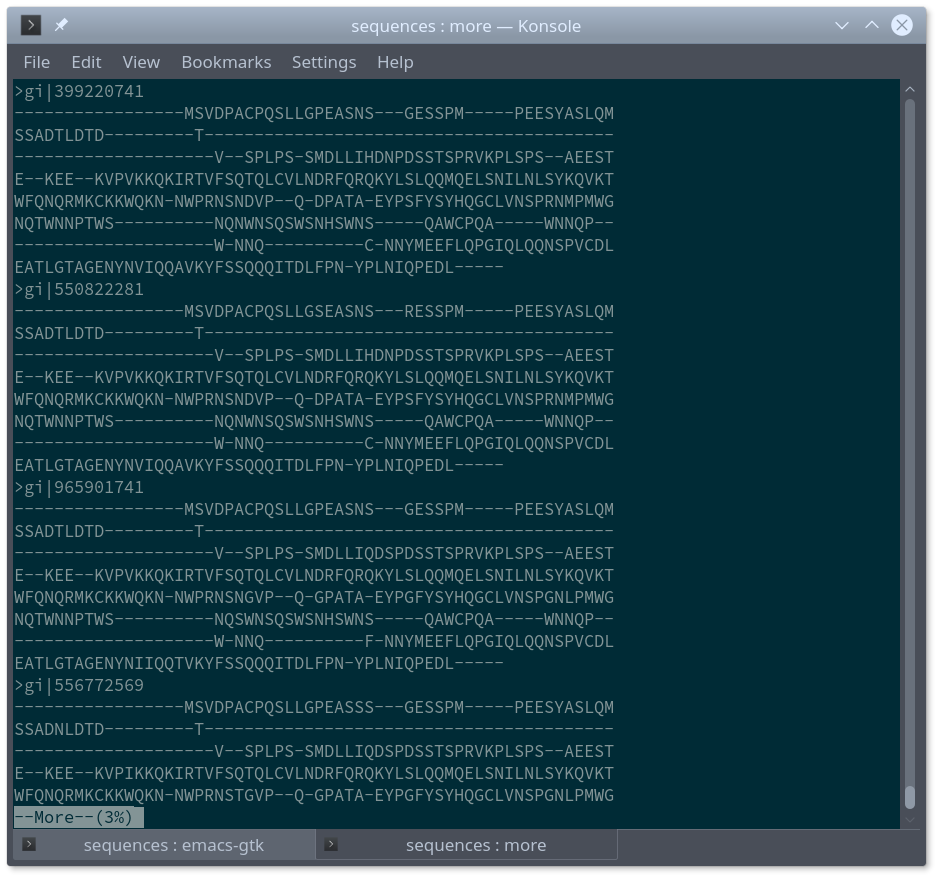
\includegraphics[width=0.8\textwidth]{images/ncbi_blink_8}
  \end{figure}
  
\end{frame}

\begin{frame}{Your own blast?}
  \begin{figure}[ht]
    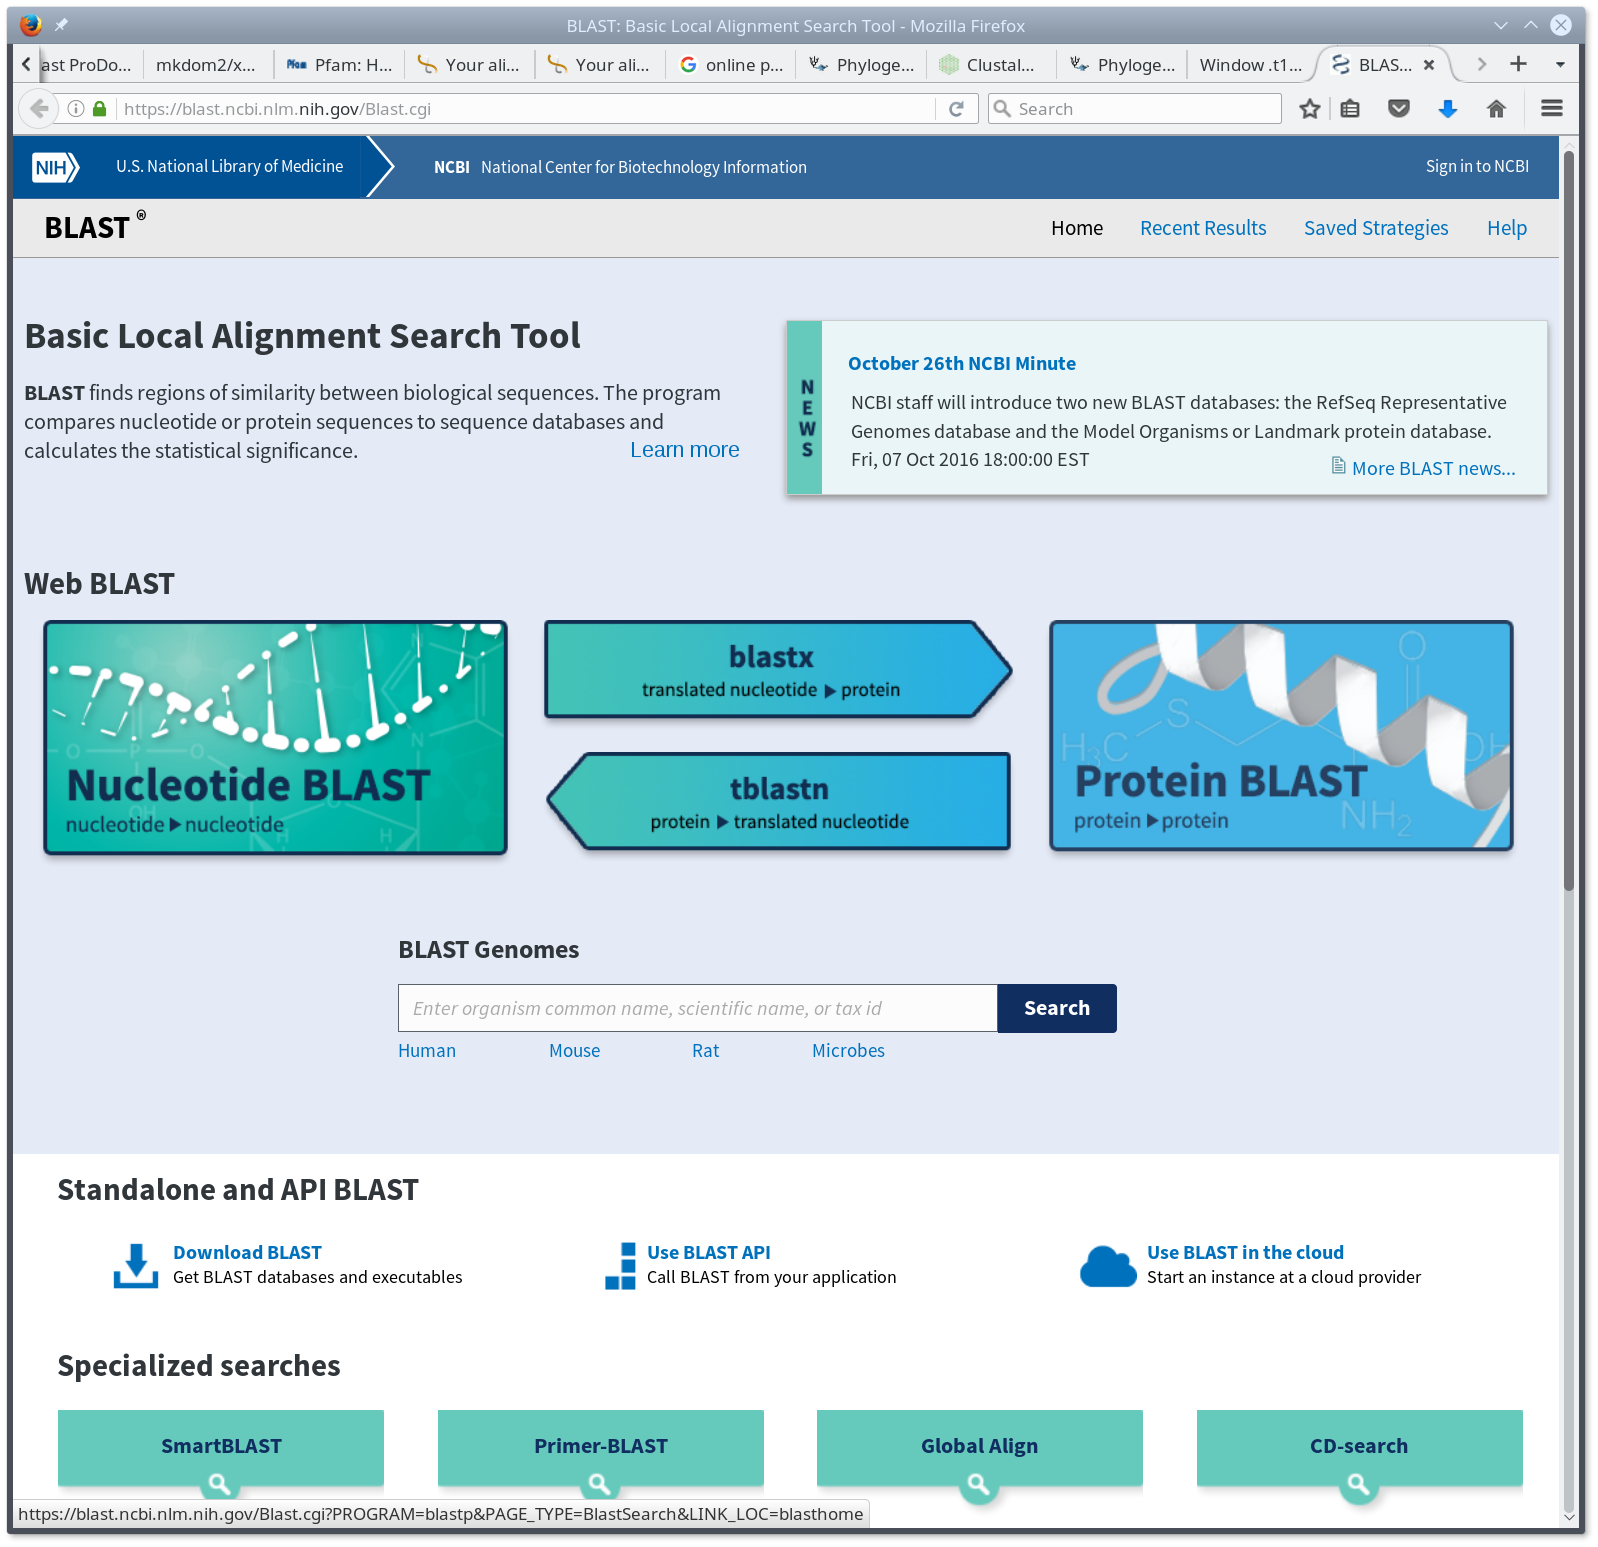
\includegraphics[width=0.8\textwidth]{images/ncbi_blast_1}
  \end{figure} 
\end{frame}

\begin{frame}{Specialised blast}
  \begin{figure}[ht]
    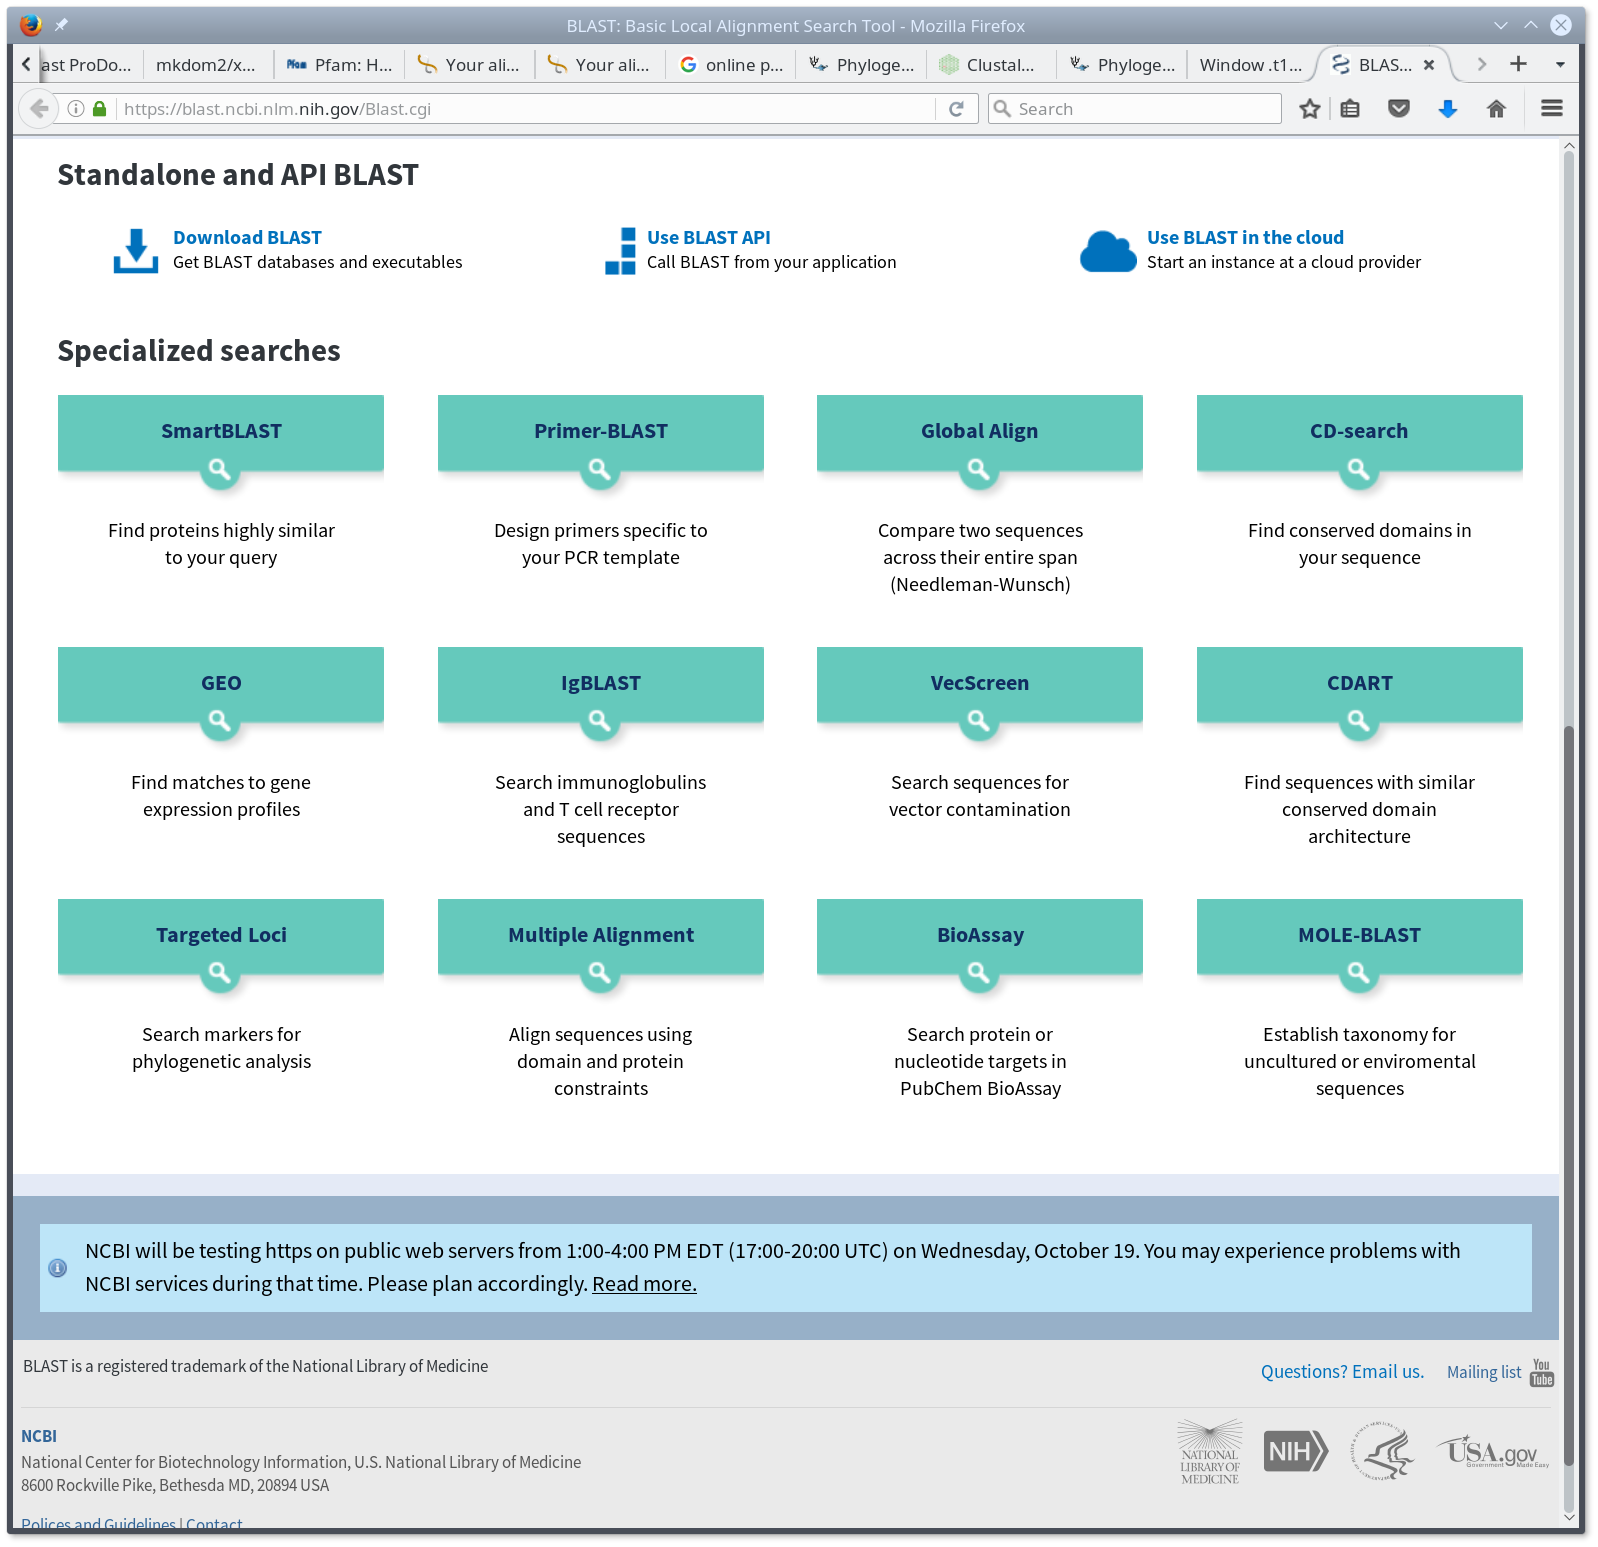
\includegraphics[width=0.7\textwidth]{images/ncbi_blast_2}
  \end{figure} 
  too many options
\end{frame}

\begin{frame}{TBLASTN}
\footnotesize  Protein query $\Rightarrow$ Translated nucleotide databases\\
Mouse nanog protein sequence against genomes!
  \begin{figure}[ht]
    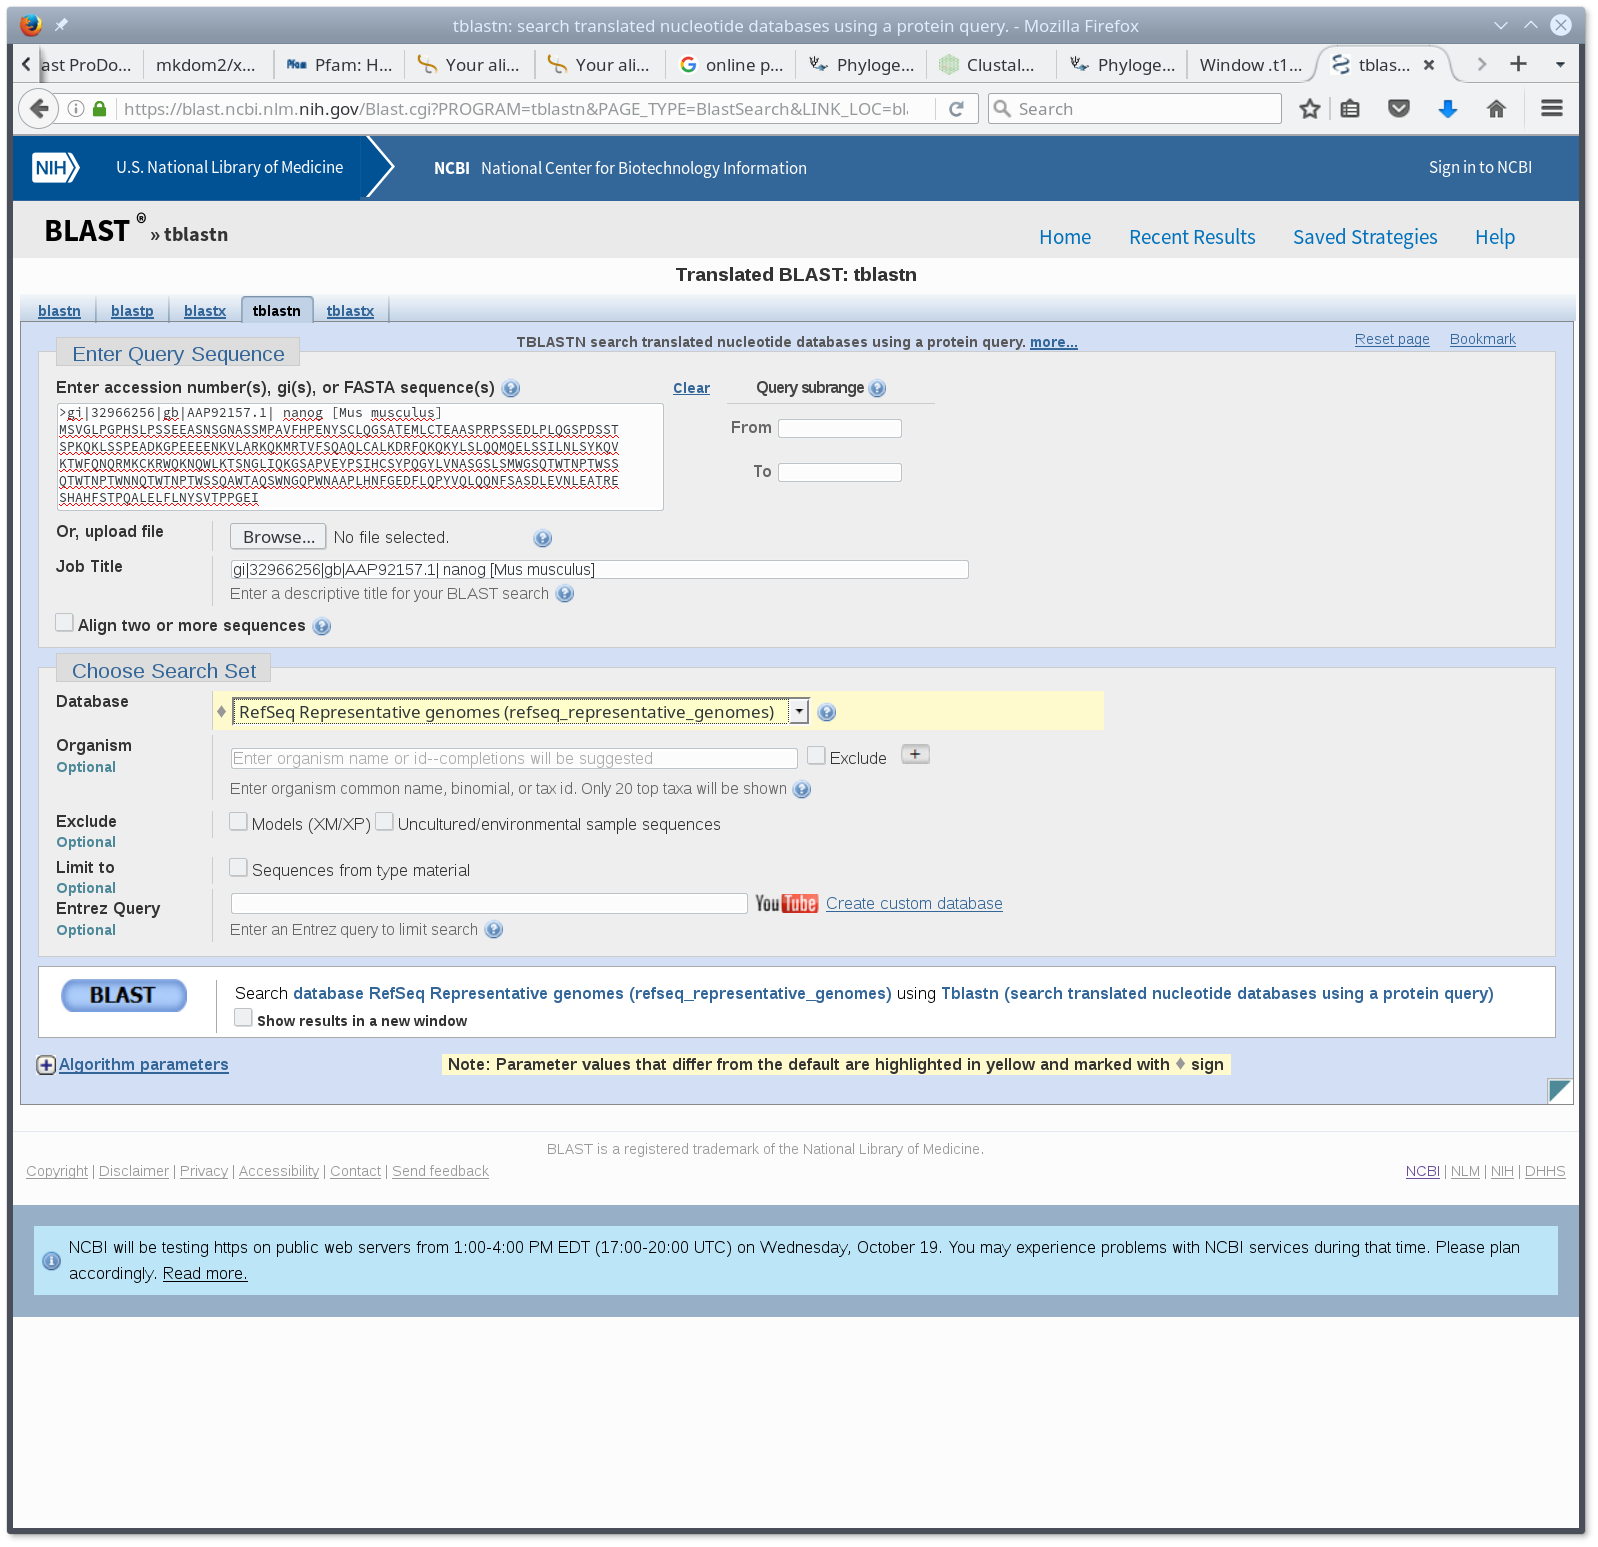
\includegraphics[width=0.75\textwidth]{images/ncbi_blast_3}
  \end{figure} 
\end{frame}

\begin{frame}{TBLASTN: parameters}
  \begin{figure}[ht]
    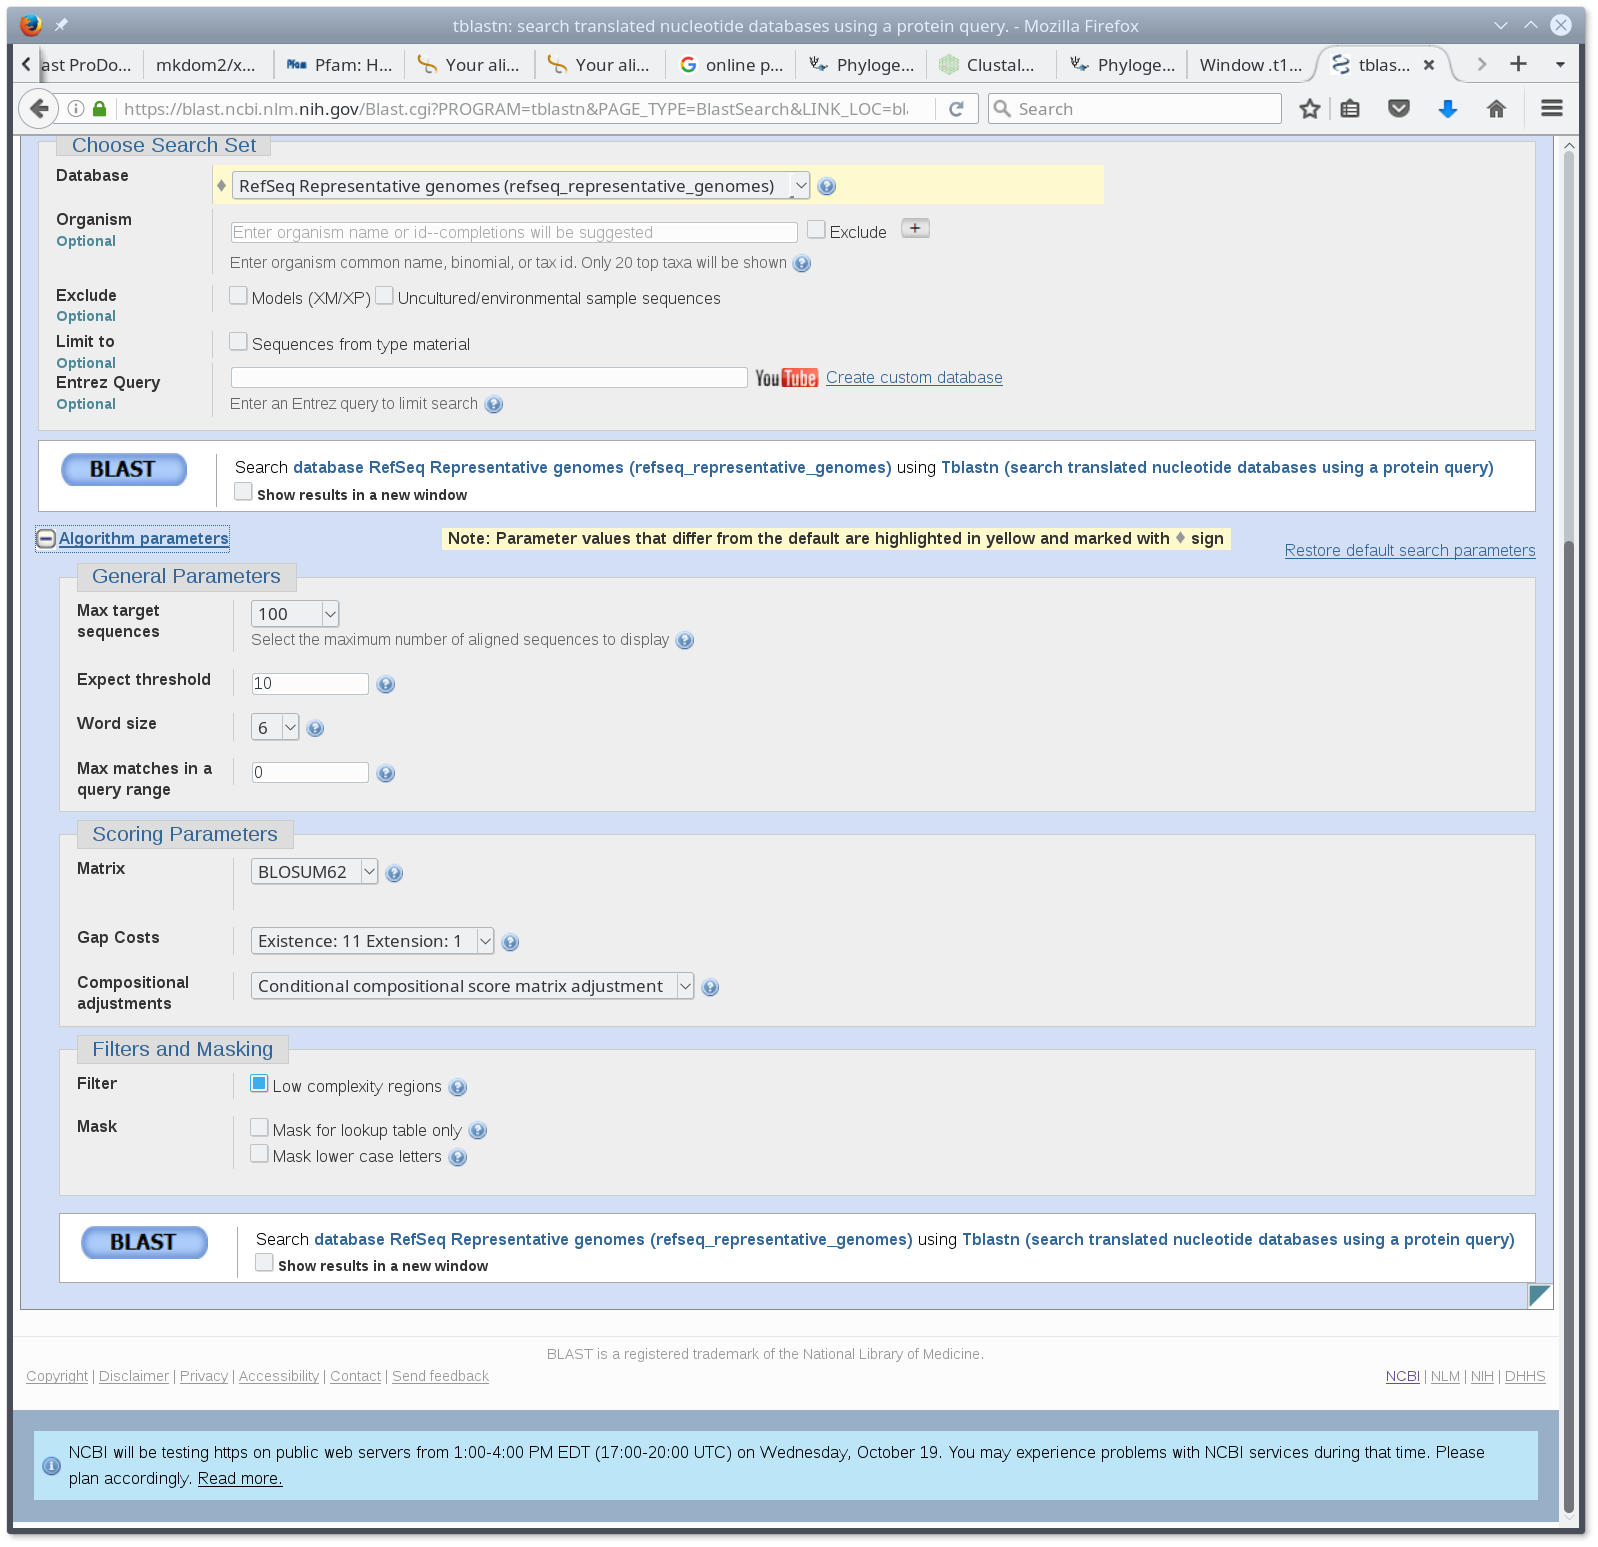
\includegraphics[width=0.75\textwidth]{images/ncbi_blast_4}
  \end{figure} 
\end{frame}

\begin{frame}{TBLASTN: results}
  ok, this one is too expensive. Still running.
\end{frame}

\begin{frame}{PSI-blast}
  You have already heard of:
  \begin{itemize}
  \item blastn
  \item blastp
  \item tblastn
  \item blastx
  \item tblastx
  \end{itemize}

  PSI-blast is a specific variant of protein blast designed to find distant homologues.

\end{frame}

\begin{frame}{PSI-blast}
  PSI-blast works by:
  
  \begin{enumerate}
  \item Blast protein against protein database using a standard amino acid
    substitution matrix.
  \item Align all hits having an e-value below a given threshold.
  \item Count the number of each amino acid at each position in the alignment
  \item Create a new amino-acid substitution matrix for each position based on
    the frequency of amino acids (i.e. a Position-Specific substitution
    matrix).
  \item Blast all sequences using the new matrix.
  \item Build a new Position-Specific substitution matrix from all alignments
    with an acceptable e-value.
  \item Go to 5, until no new sequences are identified.
  \end{enumerate}
\end{frame}

\begin{frame}{PSI-blast}
  \begin{figure}[ht]
    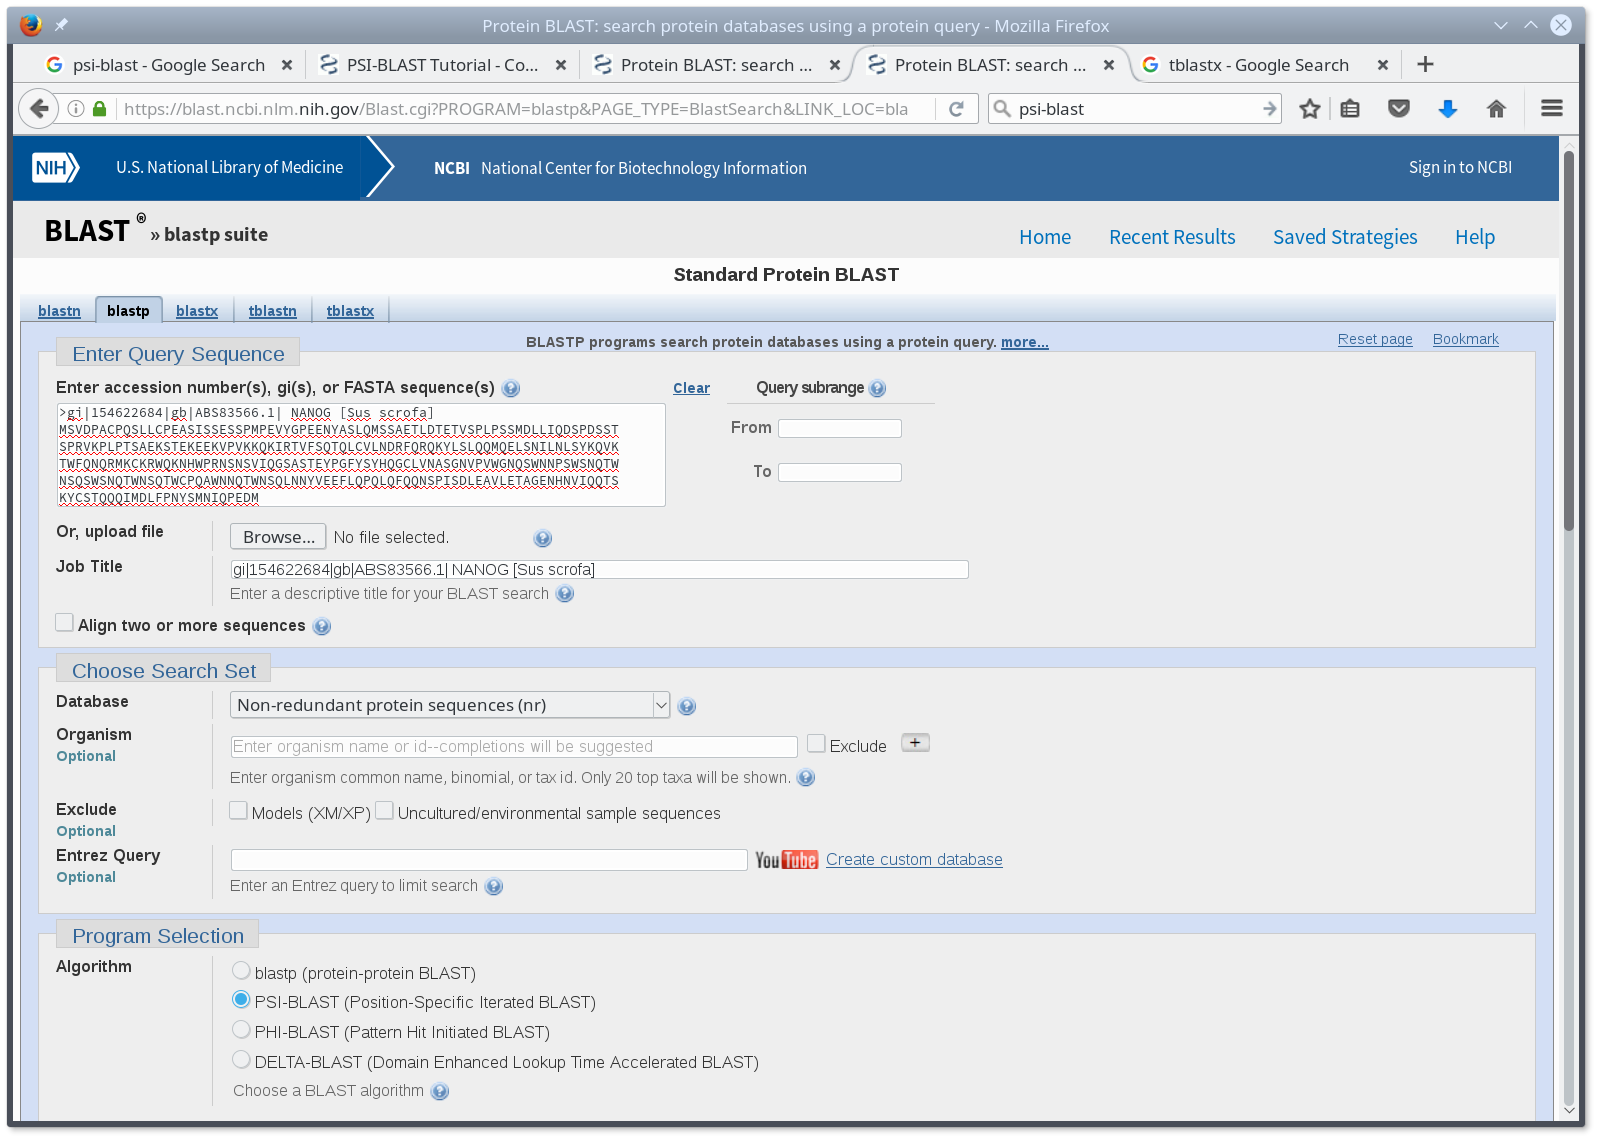
\includegraphics[width=0.8\textwidth]{images/ncbi_psi_blast_1.png}
  \end{figure}
\end{frame}

\begin{frame}{PSI-blast paramters}
  \begin{figure}[ht]
    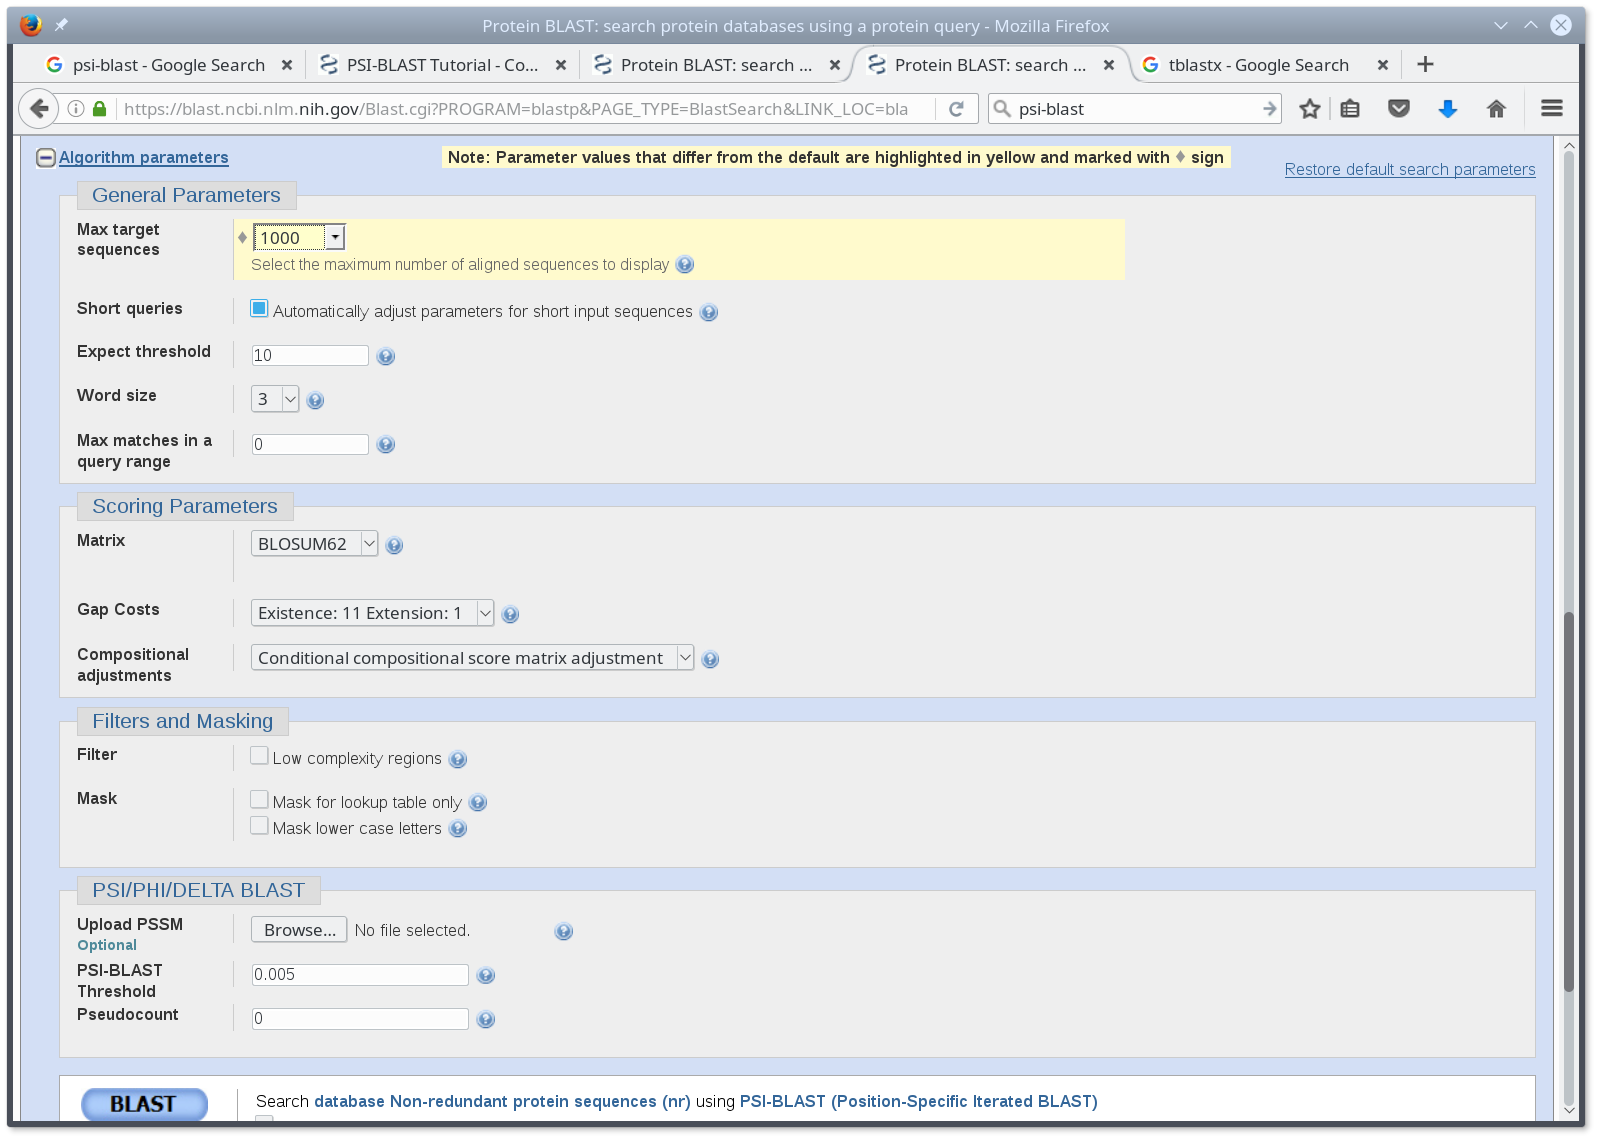
\includegraphics[width=0.8\textwidth]{images/ncbi_psi_blast_2.png}
  \end{figure}
\end{frame}

\begin{frame}{PSI-blast results run 1}
  \begin{figure}[ht]
    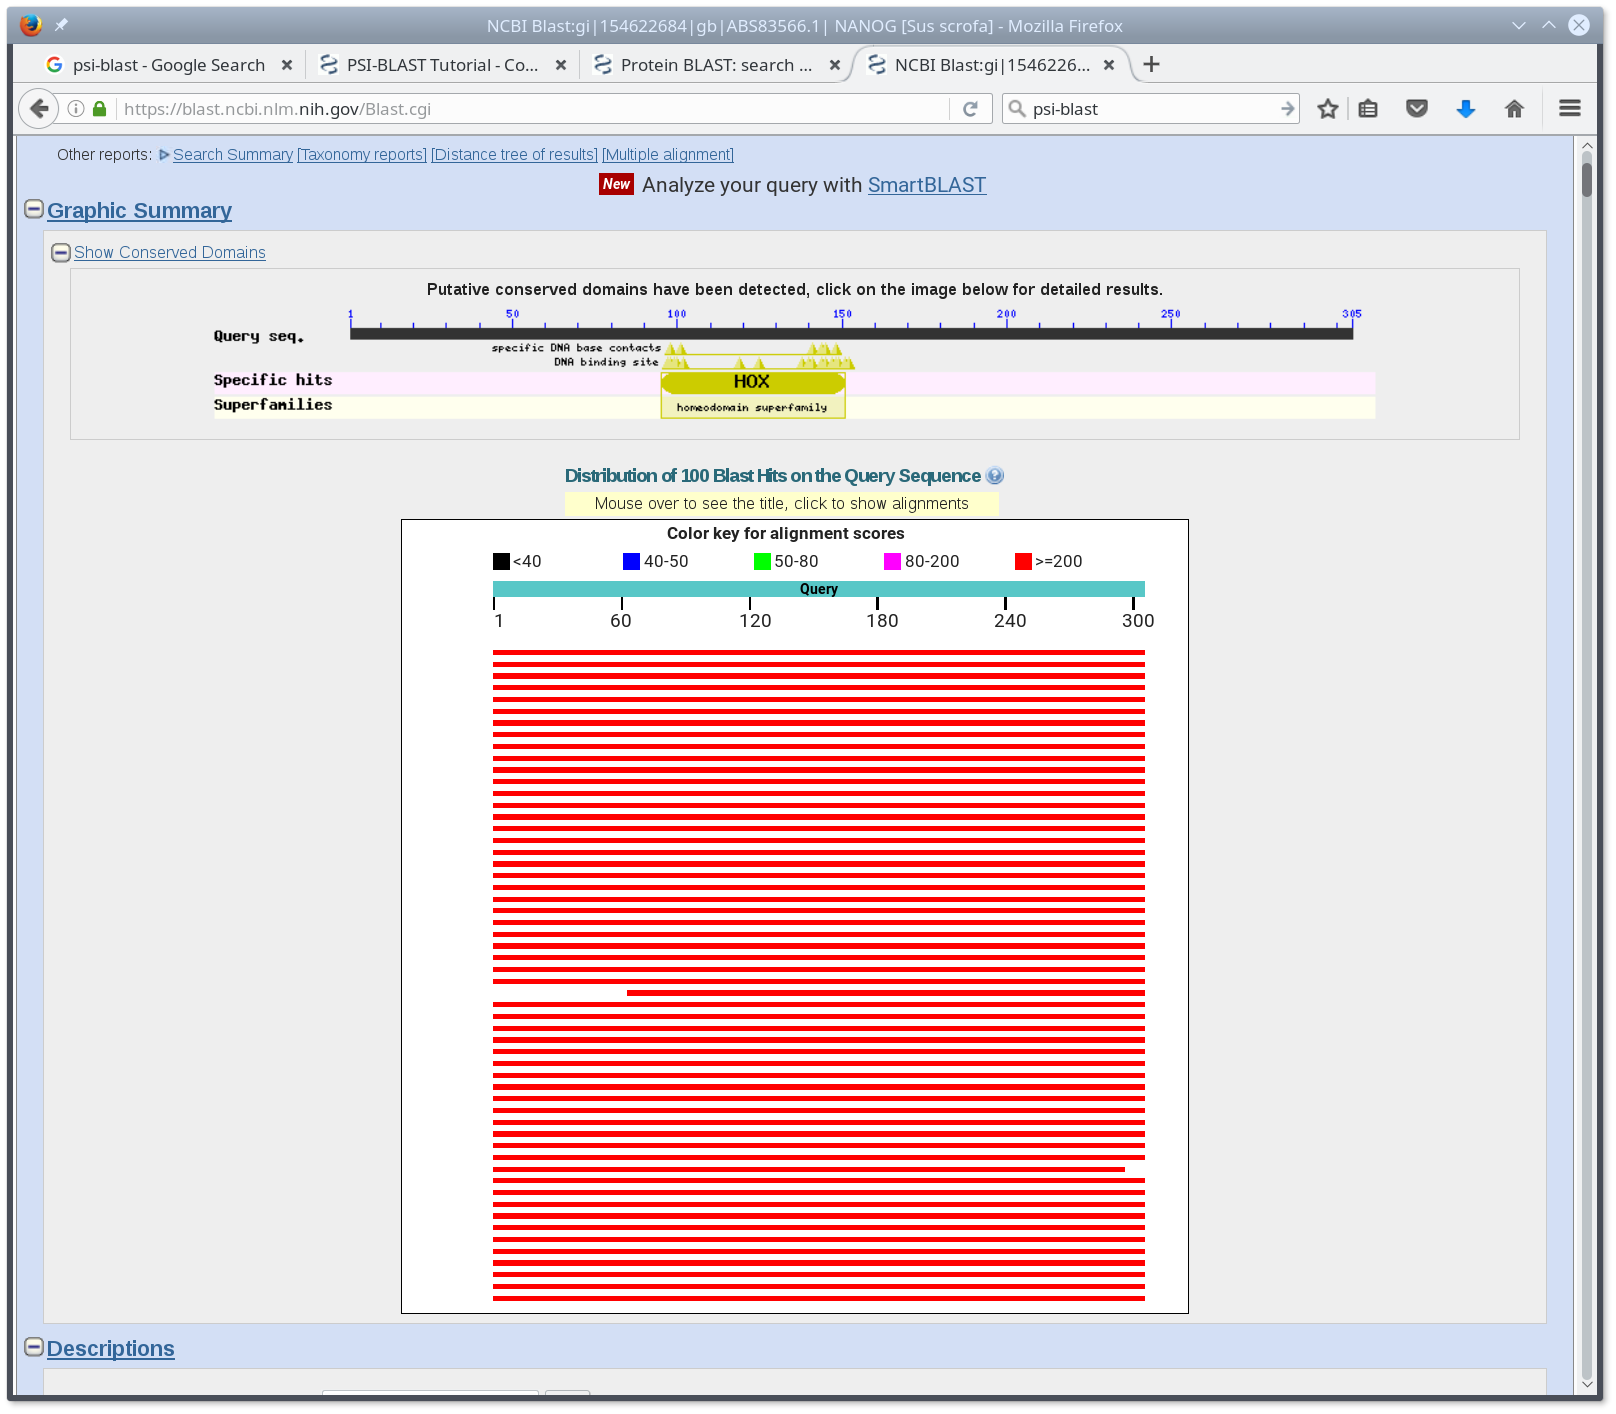
\includegraphics[width=0.7\textwidth]{images/ncbi_psi_blast_3.png}
  \end{figure}
\end{frame}

\begin{frame}{PSI-blast re-iterate}
  \begin{figure}[ht]
    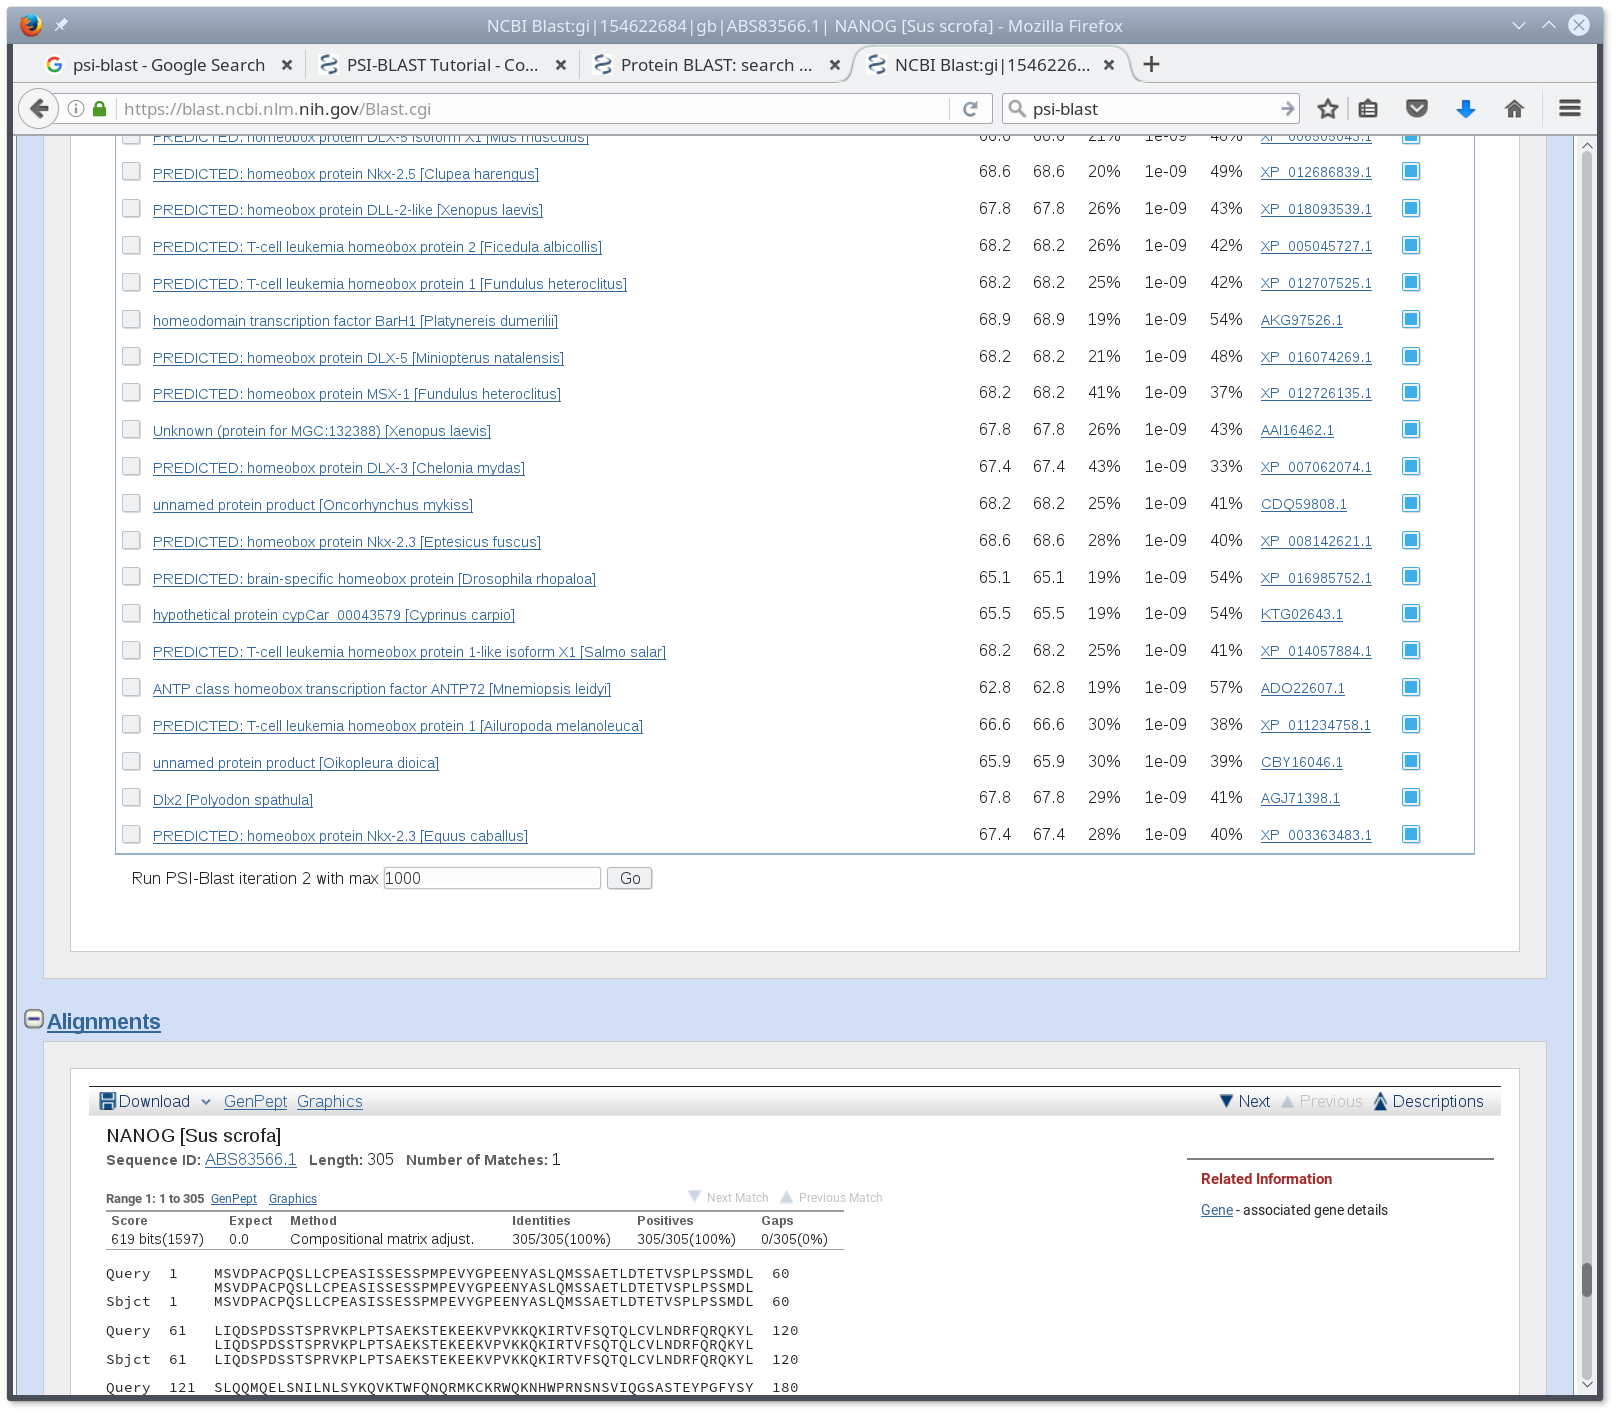
\includegraphics[width=0.7\textwidth]{images/ncbi_psi_blast_4.png}
  \end{figure}
\end{frame}

\begin{frame}{PSI-blast results run 1}
  \begin{figure}[ht]
    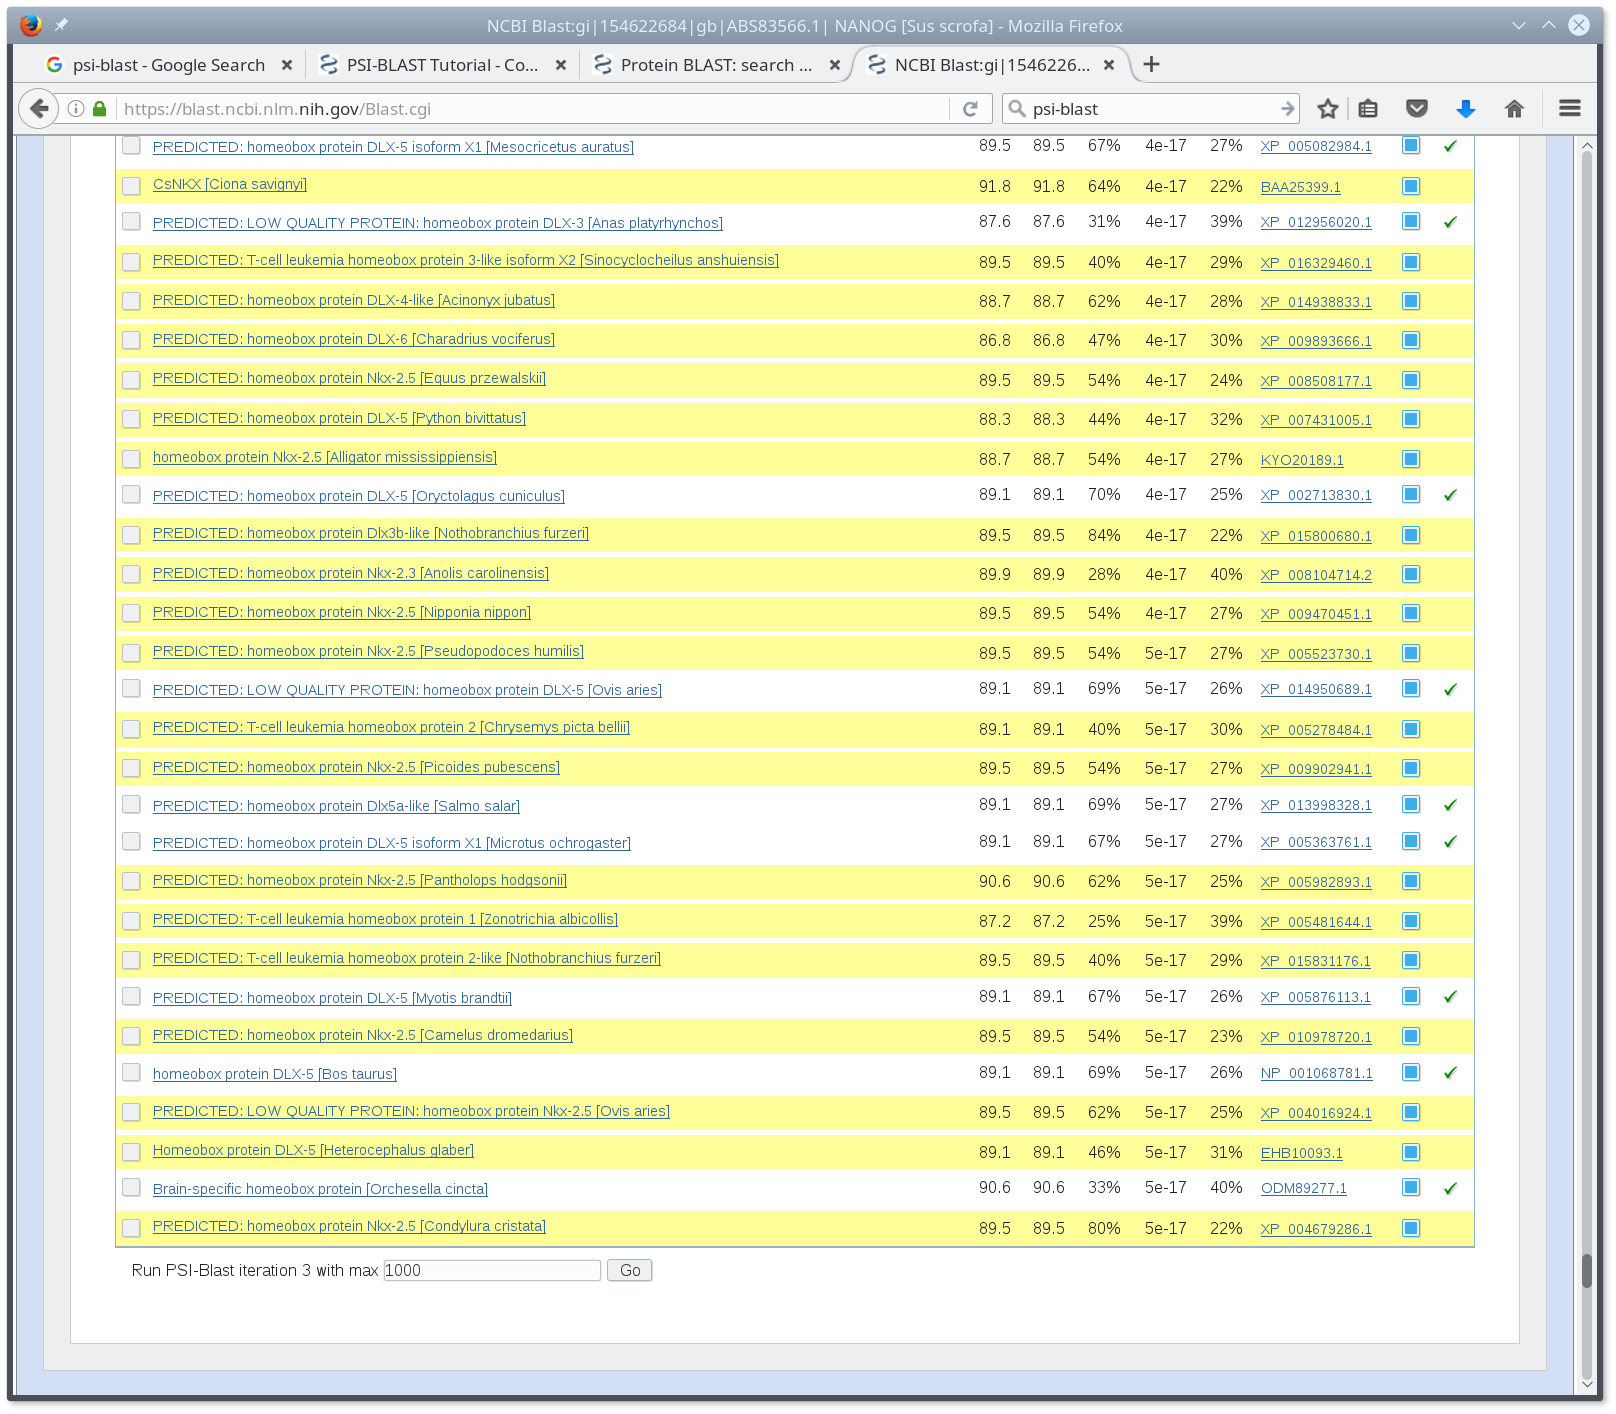
\includegraphics[width=0.7\textwidth]{images/ncbi_psi_blast_5.png}
  \end{figure}
\end{frame}

\begin{frame}{PSI-blast}
  \begin{itemize}
  \item Progressive increase in the number of homologous sequences identified for a
  given e-value.
  \item Identifies progressively more distant orthologues.
  \item Can be used to identify the evolutionary constraints of the sequences.
  \end{itemize}

  but web interface doesn't even tell me how many homologues identified at
  each iteration. Still need to download raw data to do something useful...
\end{frame}

\begin{frame}{too many tools}
  \begin{itemize}
  \item both the interfaces and the number of tools changing rapidly.
  \item no fixed information; have to try things out as they become available
  \item  offline (generally command-line) tools do not change as quickly and are
  hence often more convenient to use.
  \end{itemize}

  Main advantage of online tools is that they generally use the most up to
  date database versions.
\end{frame}

\end{document}
